% wfs_chapter_hda
% - git repository https://github.com/spatialaudio/wfs_chapter_hda
% - drafts for the chapters (english, german) on **Wave Field Synthesis** for
% Stefan Weinzierl (ed.): *Handbuch der Audiotechnik*, 2nd ed., Springer,
% https://link.springer.com/referencework/10.1007/978-3-662-60357-4
% - text and graphics under CC BY 4.0 license https://creativecommons.org/licenses/by/4.0/
% - source code under MIT license https://opensource.org/licenses/MIT
% - Springer has copyright to the final english / german chapters and their layouts
% - we might also find https://git.iem.at/zotter/wfs-basics useful
% - we use violine image from https://upload.wikimedia.org/wikipedia/commons/thumb/f/f1/Violin.svg/2048px-Violin.svg.png to create picture `python/violin_wfs.png`

% Authors:
% - Frank Schultz, https://orcid.org/0000-0002-3010-0294, https://github.com/fs446
% - Nara Hahn, https://orcid.org/0000-0003-3564-5864, https://github.com/narahahn
% - Sascha Spors, https://orcid.org/0000-0001-7225-9992, https://github.com/spors

\section{Einleitung}
\label{sec:WFSIntro}
%
Wellenfeldsynthese (WFS)\index{Wellenfeldsynthese} \cite{Vries2009_Mono, Sporer2018_book}
ist ein nicht-kanalbasiertes Lautsprecherwiedergabeverfahren, welches in der Praxis
häufig zur Spatialisierung von Audio-Objekten verwendet wird \cite{Ranjan2013_IEEE}.
%
Mit einer großen Anzahl dicht gereihter und individuell ansteuerbarer Lautsprecher
werden Überlagerungen von Wellen, d.h. Interferenzen, kontrolliert erzeugt,
so dass gewünschte Wellenfrontenverläufe\index{Wellenfront}
entstehen, vgl.~\Abb\ref{fig:violine}~(rechts) und \Abb\ref{fig:td_0m}.
%
% Nara Diskussion: sauber Wellenfront (für 3D und 2.5D) vs. Wellenfeld (nur für 3D)
% definieren->guter Punkt.
% Wellenfrontenverläufe meint implizit einmal Wellenfeld mit Abb. 2
% und wird in Folge dann
% zu Gunsten von Wellenfront (Abb. 17!) nur noch einmal benutzt: beim Paragraph
% Namensgebung, wo man sich nochmal wundern darf über die Unterschiede
Die WFS wird den sogenannten \index{Schallfeldsynthese}Schallfeldsyntheseverfahren
zugeordnet \cite{Spors2013_IEEE}
%
und für Audioanwendungen seit Ende der 1980er Jahre \cite{Berkhout1988_JAES}
erforscht und entwickelt.
%
In der Praxis werden meist horizontale, zuhörerflächen-(teil)-umschließende
Lautsprecherarrays verwendet, also z.B. Rechteck-, Kreisarrays oder frontale
Zeilen, vgl.~\Abb\ref{fig:WFS_Array_Haus8} und \cite{Vries2009_Mono, Vries2019}.



In diesem Kapitel wird die Grundidee der WFS aufgezeigt.
%
Im Rest dieses Abschnitts wird das WFS-Konzept grundlegend verortet
und der Wissensstand zur WFS historisch kurz eingeordnet.
%
In \Kap{sec:WFSFundamentals} wird das wellentheoretische Fundament der WFS eingeführt.
%
Danach wird in \Kap{sec:WFS_PointSource} eine kompakte, allgemeine Herleitung
für die WFS einer virtuellen Punktquelle präsentiert.
%
Mit numerischen Simulationen werden in \Kap{sec:WFS_PointSource_Simulationen}
die wichtigsten Eigenschaften der mit WFS
erzeugten Schallfelder und einige psychoakustische Implikationen diskutiert.
%
Der \Kap{sec:mods_25d_wfs} behandelt einige praxisrelevante
Modifikationen und Erweiterungen.
%
Abschließend wird in \Kap{sec:WFS_Werkzeuge} kurz auf Werkzeuge für die
Produktionspraxis eingegangen.
%
% please DO NOT rescale the figure and keep it double column
\begin{figure*}
\centering
\begin{plotfigures}
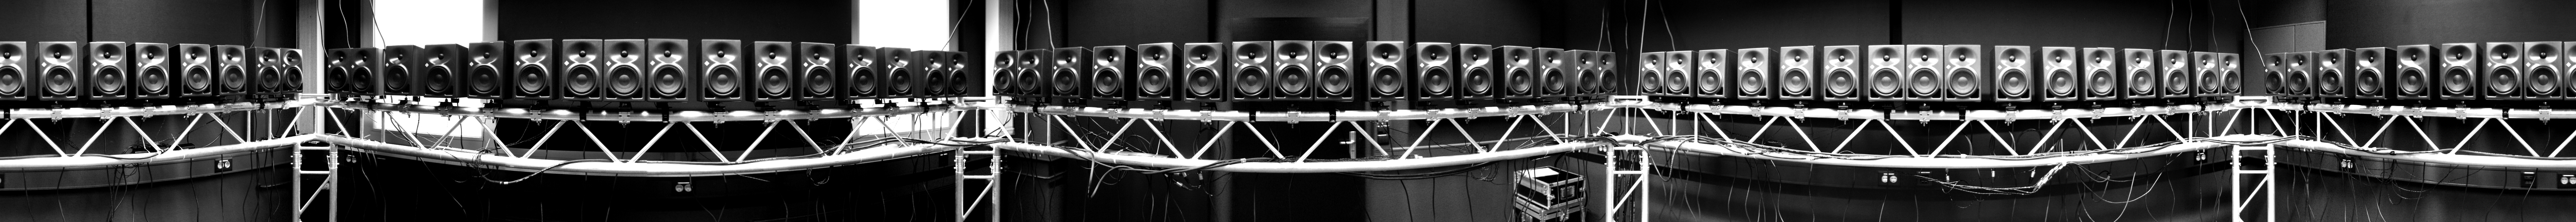
\includegraphics[width=174mm]{../fotos/WFS_Array_UniRostockH8_2014.jpg}
\end{plotfigures}
\caption{Panoramafoto des WFS-Systems im Audio-Labor der Universität Rostock mit
64 Zwei-Weg-Studiomonitoren auf Ohrhöhe für mittelgroße, stehende Zuhörende und
entlang einer $4 \text{m} \times 4 \text{m}$ quadratischen Hüllkontur mit freien
Ecken und mittlerem Lautsprecherabstand von ca. $0{,}23$\,m.
%
CC BY 4.0 Matthias Geier, Sascha Spors.
}
\label{fig:WFS_Array_Haus8}
\end{figure*}



Bei der WFS steht zunächst die
technisch optimierte Erzeugung von Wellenfronten für einen großen
Zuhörerbereich im Vordergrund.
%
Dem Verfahren liegt die Annahme zugrunde, dass technisch perfekt synthetisierte
Wellenfronten, vgl.~\Abb\ref{fig:violine}~(rechts)
identisch zu Referenzwellenfronten, vgl.~\Abb\ref{fig:violine}~(links) sind,
sie daher die gleiche binaurale Anregung \cite[S.\,573]{Snow1953} und
auditive Wahrnehmung zur Folge haben.
%
Bei perfekter Synthese lässt sich die Erzeugung von akustischen Szenen
aus Wellenfronten als rein technisches Herstellungsverfahren auffassen.
%
Die perfekte Synthese von Wellenfronten ließe sich für die gesamte
Audiobandbreite nur mit sehr hohem technischen Aufwand
realisieren.
%
In der Praxis muss die Wellenfronterzeugung für die gewünschte
akustische Szene im Hinblick auf
a) vertretbaren Technik- und Kostenaufwand,
b) technische und
c) perzeptive Optimierung
erfolgen.
%
Es erscheint dann sinnvoll, die WFS -- oder gar individuelle WFS-Systeme,
bestehend aus Hard- und Software -- als Instrumente aufzufassen, die es
technisch und psychoakustisch zu erforschen und erlernen gilt.
%
Dies wurde mutmaßlich erstmals in den 1930er Jahren als Ingenieursutopie
in Aussicht gestellt \cite{Fletcher1934,Steinberg1934} -- aus der zunächst
die Left/Center/Right (LCR) Wiedergabetechnik
motiviert wurde -- und dann ab
Ende der 1980er Jahre \cite{Berkhout1988_JAES} dank Realisierbarkeit mit
digitaler Echtzeitsignalverarbeitung umgesetzt.
%
% please DO NOT rescale the figure and keep it single column
\begin{figure}[b]
\centering
\begin{plotfigures}
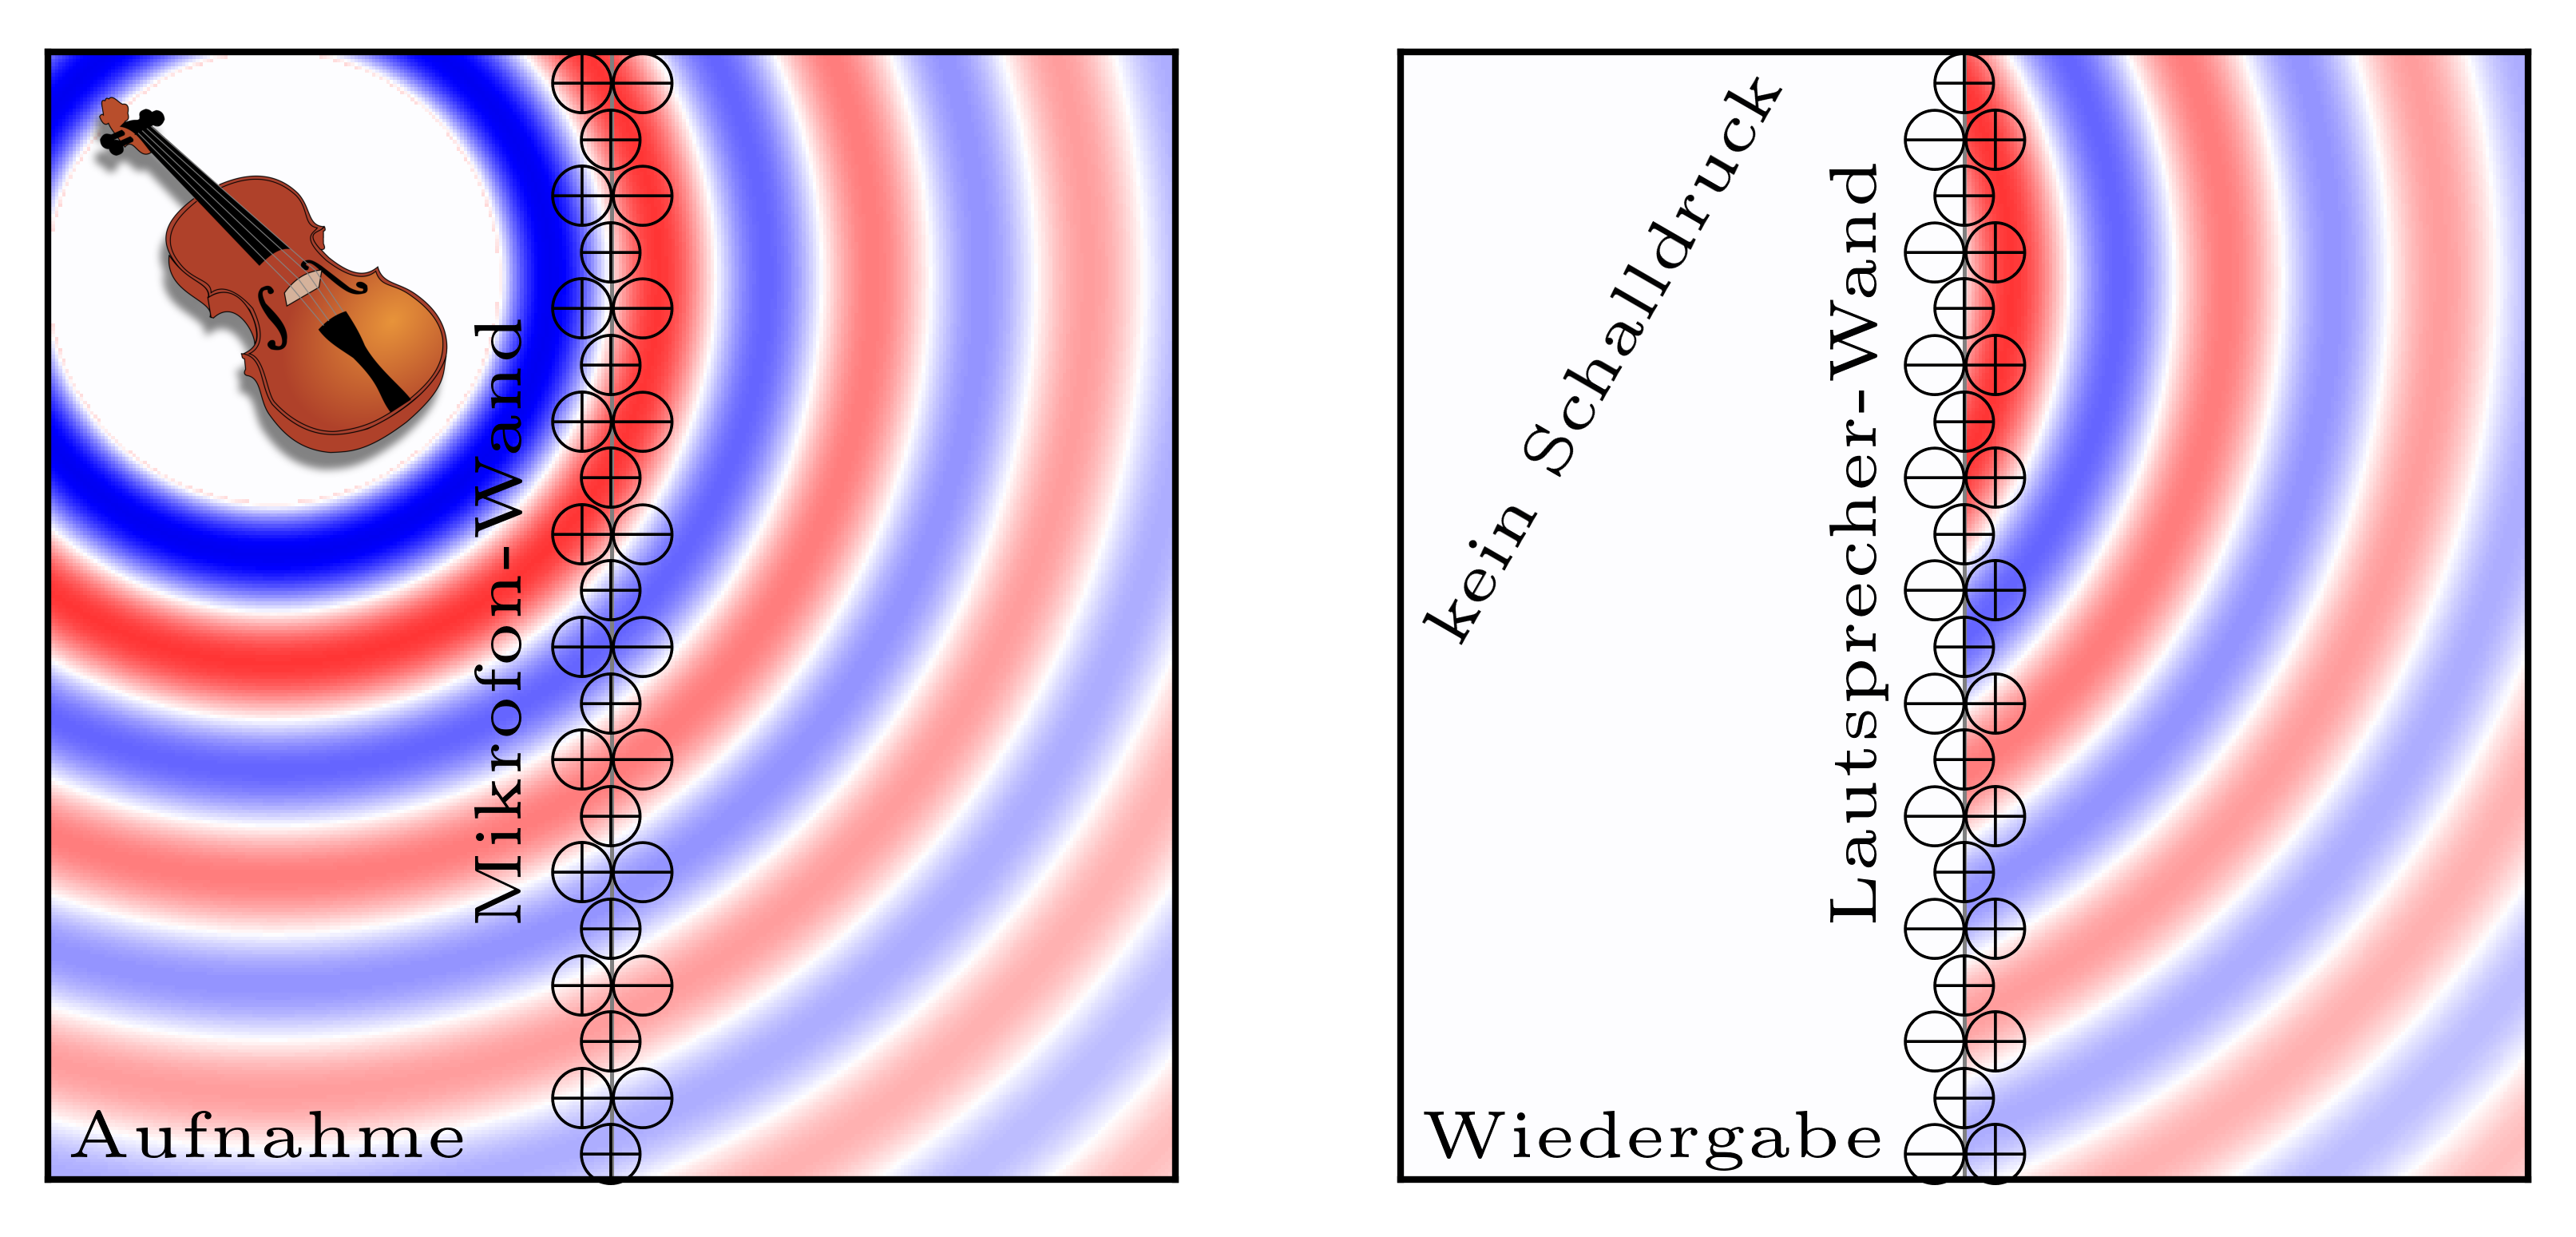
\includegraphics[width=85mm]{../python/violin_wfs_DEU.png}
\end{plotfigures}
\caption{WFS-Prinzip basierend auf der \Glg\eqref{eq:KHIGeneral} für das
Halbraumproblem.
%
Links: Aufnahme einer akustischen Szene mit Achter-Druckgradienten-
$(\oplus\ominus)$ und Druckmikrofonen $(\oplus)$ entlang einer Fläche.
%
Rechts: die Wiedergabe dieser Signale mit einer Fläche aus
Monopol- $(\oplus)$ und Dipollautsprechern
$(\ominus\oplus)$ führt wegen Wellenüberlagerung im
rechten Halbraum zum gleichen Schallfeld wie das der originalen
akustischen Szene (datenbasierte Direktwiedergabe).
%
Statt Messungen können analytische Schallfeldmodelle
bezüglich Druck und Druckgradient entlang der Fläche ausgewertet und daraus
die Ansteuerung für die Lautsprecher berechnet werden
(modellbasierte Wiedergabe). \cc
}
\label{fig:violine}
\end{figure}



In der Geschichte der WFS, vgl. \cite{Vries2009_Mono,Vries2019}
lassen sich grob drei Forschungs- und Entwicklungswellen ausmachen.
%
Die theoretische und praktische Einführung erfolgte in den 1990er Jahren
mit initial an der TU Delft durchgeführten
Arbeiten, wovon
\cite{Berkhout1993_JASA,Vogel1993_diss,Boone1995_JAES,Vries1996_JAES,Start1997_diss,Verheijen1997_diss,Sonke2000_diss}
das Wissensspektrum dieser ersten Welle charakterisieren.
%
In den 2000er Jahren folgte eine zweite Welle, die ausgehend vom
EU-Entwicklungsprojekt CARROUSO \cite{Brix2001}
von Bemühungen zur Standardisierung (MPEG4) \cite{Plogsties2003}
und Vermarktung
(Firmen Iosono und Sonic Emotions) geprägt war.
%
WFS wurde als Wiedergabeverfahren für ein breites Feld von potentiellen
Anwendungsszenarien \cite{Sporer2004a, Theile2003}
diskutiert.
%
Technische Aspekte wurden im Detail untersucht \cite{Apel2004,Hulsebos2004_diss,Spors2007b,Corteel2006_JAES,Gauthier2007_JAES,Melchior2008,Franck2008,Salvador2010},
der Instrumentencharakter von WFS wurde bezüglich tonmeisterlicher
Ästhetik \cite{Theile2003,Kuhn2003,Wittek2007_JAES,Wittek2007_diss}, als auch
hinsichtlich der Bedienungsästhetik von Audio-Objekten \cite{Melchior2003,Vaananen2003,Pellegrini2004,Baalman2008_diss}
weiter erörtert.
%
Zudem wurden in dieser Phase die Ambisonics-Derivate
%\redcol{@Edit: Verweis auf Kapitel zu Ambisonics?}
und die WFS
als objektbasierte Wiedergabeverfahren
bezüglich ihrer Gemeinsamkeiten und Unterschiede
analysiert \cite{Nicol1999,Daniel2003,Gauthier2006_JASA,Spors2008b,Ahrens2010_IEEE,Fazi2010}.
%
Die dritte Welle ab den 2010er Jahren konsolidierte und erweiterte das Verständnis
zur Theorie und Psychoakustik von
WFS vor allem mit den Arbeiten \cite{Spors2010a,Voelk2012,Zotter2013,Rohr2013_JAES,Wierstorf2014_diss,Firtha2019_diss,Winter2019_diss,Erbes2020_diss,Hahn2022_JAES}.



\section{Grundlagen}
\label{sec:WFSFundamentals}
%
Die WFS leitet sich aus fundamentalen Gesetzen linearer Wellenausbreitung ab.
%
Diese werden in diesem Abschnitt formal eingeführt und die WFS diesbezüglich
verortet.



\subsection{Elementarquellen Mono- und Dipol}
%
% please DO NOT rescale the figure and keep it single column
\begin{figure}[b]
\centering
\begin{plotfigures}
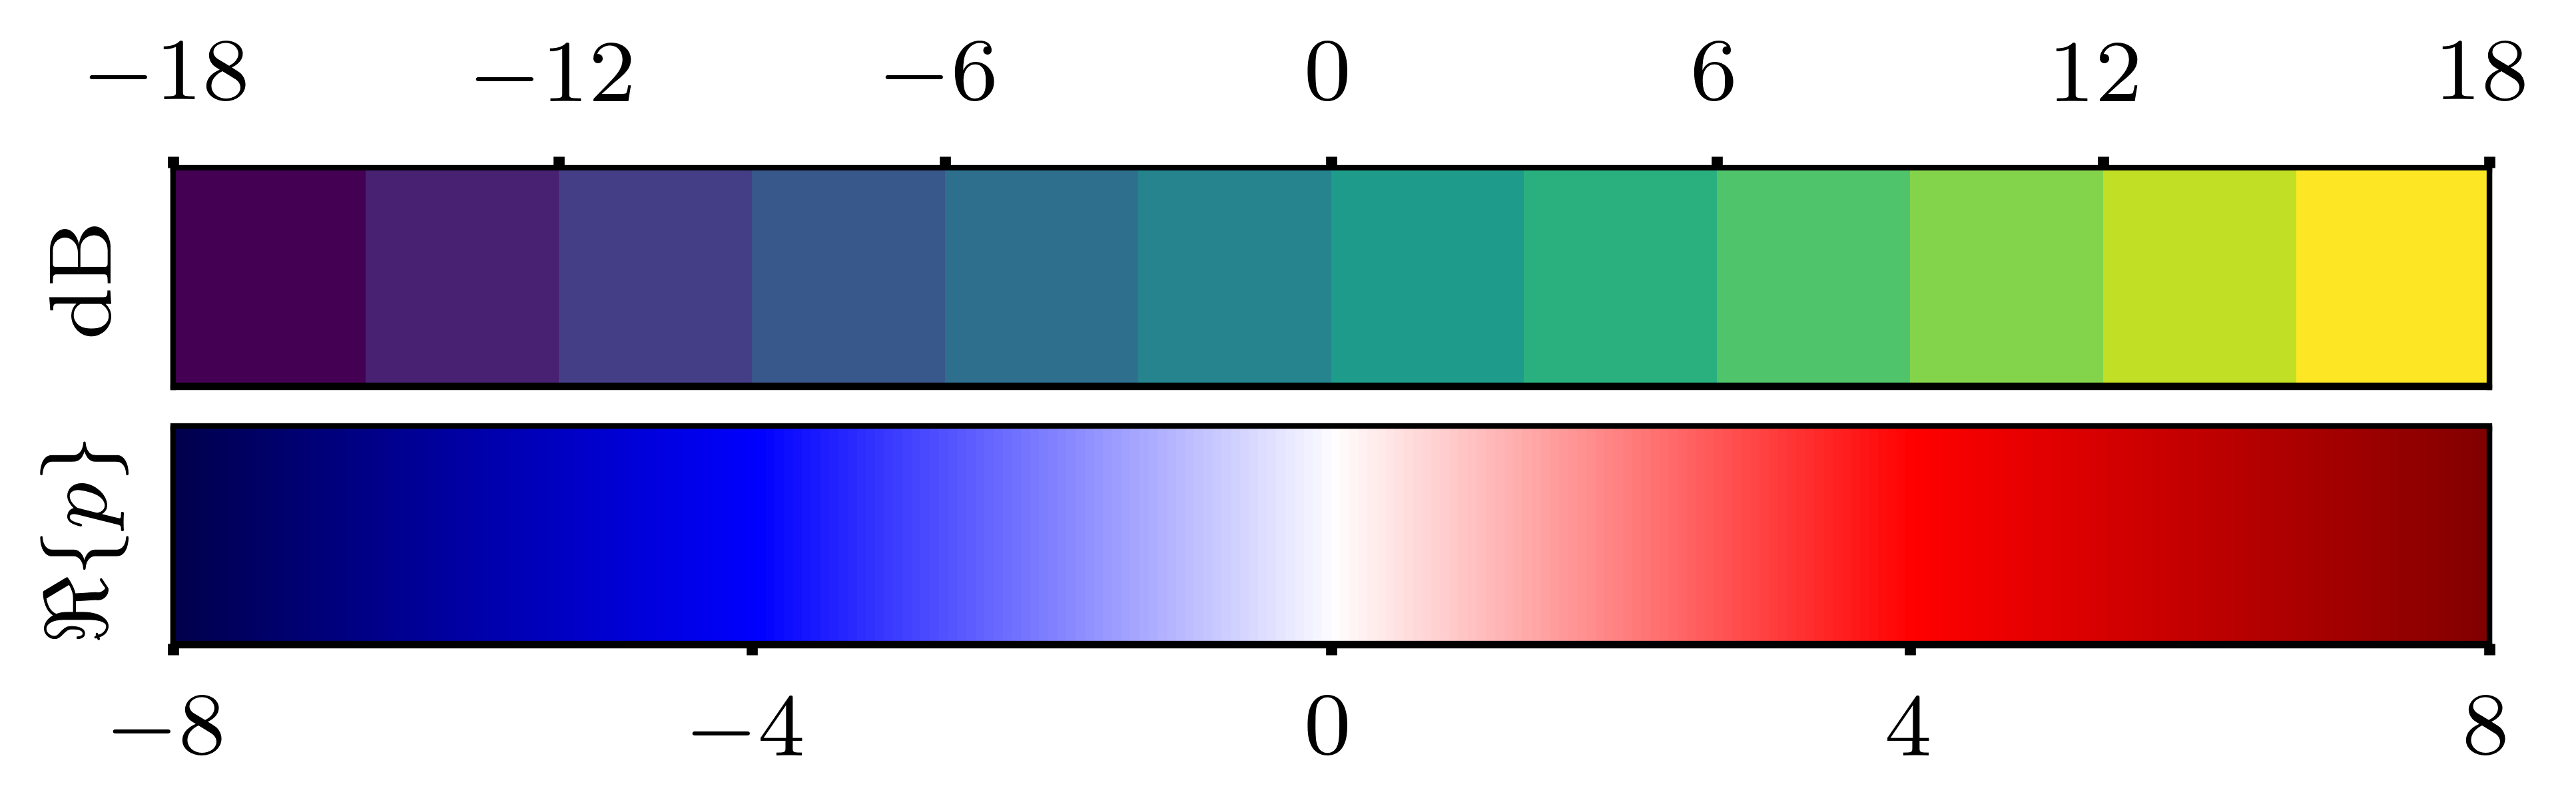
\includegraphics[width=85mm]{../python/plot_colorbar.png}
\end{plotfigures}
\caption{Farbskalierung für alle folgenden Grafiken monofrequenter
Schallfelder.
%
Oben: Pegel mit $3$\,dB pro Farbe und $0$\,dB bezogen auf Amplitudenwert Eins.
%
Unten: Realteil der komplexen Schalldruckwechselgröße $p(x_\mathrm{r},y_\mathrm{r})$.
%
Schalldruckpegel $>+18\,\text{dB}$ und Schalldruckwerte $>+8$ erfahren eine
orange Farbsättigung,
Schalldruckpegel $<-18\,\text{dB}$ und Schalldruckwerte $<-8$ sind mit cyan
gesättigt.
%
\cc
}
\label{fig:plot_colorbar}
\end{figure}
%
Zur Herleitung der WFS werden die zwei
akustischen, idealisierten Elementarquellen Monopol\index{Monopol}
und Dipol\index{Dipol} benötigt.
%
Der Monopol, auch Punktquelle genannt, an der Position $\xs=(x,y,z)^\mathrm{T}$
erzeugt ein monofrequentes 3D-Schallfeld
\begin{align}
\label{eq:G03D}
G(r_{\xs\text{-}\xr})=\frac{\e^{-\im\wc r_{\xs\text{-}\xr}}}{4\pi \, r_{\xs\text{-}\xr}}
\end{align}
für die Empfänger-/Mess-/Aufpunkte
$\xr=(x_\mathrm{r},y_\mathrm{r},z_\mathrm{r})^\mathrm{T}$.
%
Die $\frac{1}{4 \pi}$--Normalisierung ist gewählt, damit unten
\Glg\eqref{eq:KHIGeneral} in dieser Form eingeführt werden kann.
%
Die als konstant angenommene Schallausbreitungsgeschwindigkeit $c$ [m/s] ergibt
sich als Produkt von Frequenz $f$ [Hz] und
akustischer Wellenlänge $\lambda$ [m]
\begin{align}
c = \lambda f,
\end{align}
und es besteht der Zusammenhang
%\begin{align}
$\omega = 2 \pi f$
%\end{align}
zwischen Kreisfrequenz $\omega$ [rad/s] und Frequenz $f$.
%
Die imaginäre Zahl $\im$ liefert nach Definition $\im^2=-1$.
%
Der Abstand zwischen der Quellenposition $\xs$ und einem Messpunkt $\xr$ wird mit
$r_{\xs\text{-}\xr}=\|\xs-\xr\|$ beschrieben.
%
Die euklidische Länge eines kartesischen Vektors $\bm{x}$ ist als
$\|\bm{x}\|=\sqrt{x^2+y^2+z^2}$ definiert.
%
Ein Spaltenvektor $\xs$ transponiert ergibt den Zeilenvektor $\xs^\mathrm{T}$.
%
Für die in der linearen Akustik übliche Rechnung mit komplexen Zeigern für
monofrequente Schallfelder lässt sich der Schalldruckverlauf des Monopols über
die Zeit für die gewählte Kreisfrequenz $\omega$  durch Realteilbildung
$\Re\{G(r_{\xs\text{-}\xr})\cdot\e^{+\im \omega t}\}$
berechnen.
%
Für breitbandige Anwendungen wird später die Diskussion auf Spektren, z.B. für
$G(r_{\xs\text{-}\xr}, \omega)$, erweitert.


% please DO NOT rescale the figure and keep it single column
\begin{figure}[t]
\centering
\begin{plotfigures}
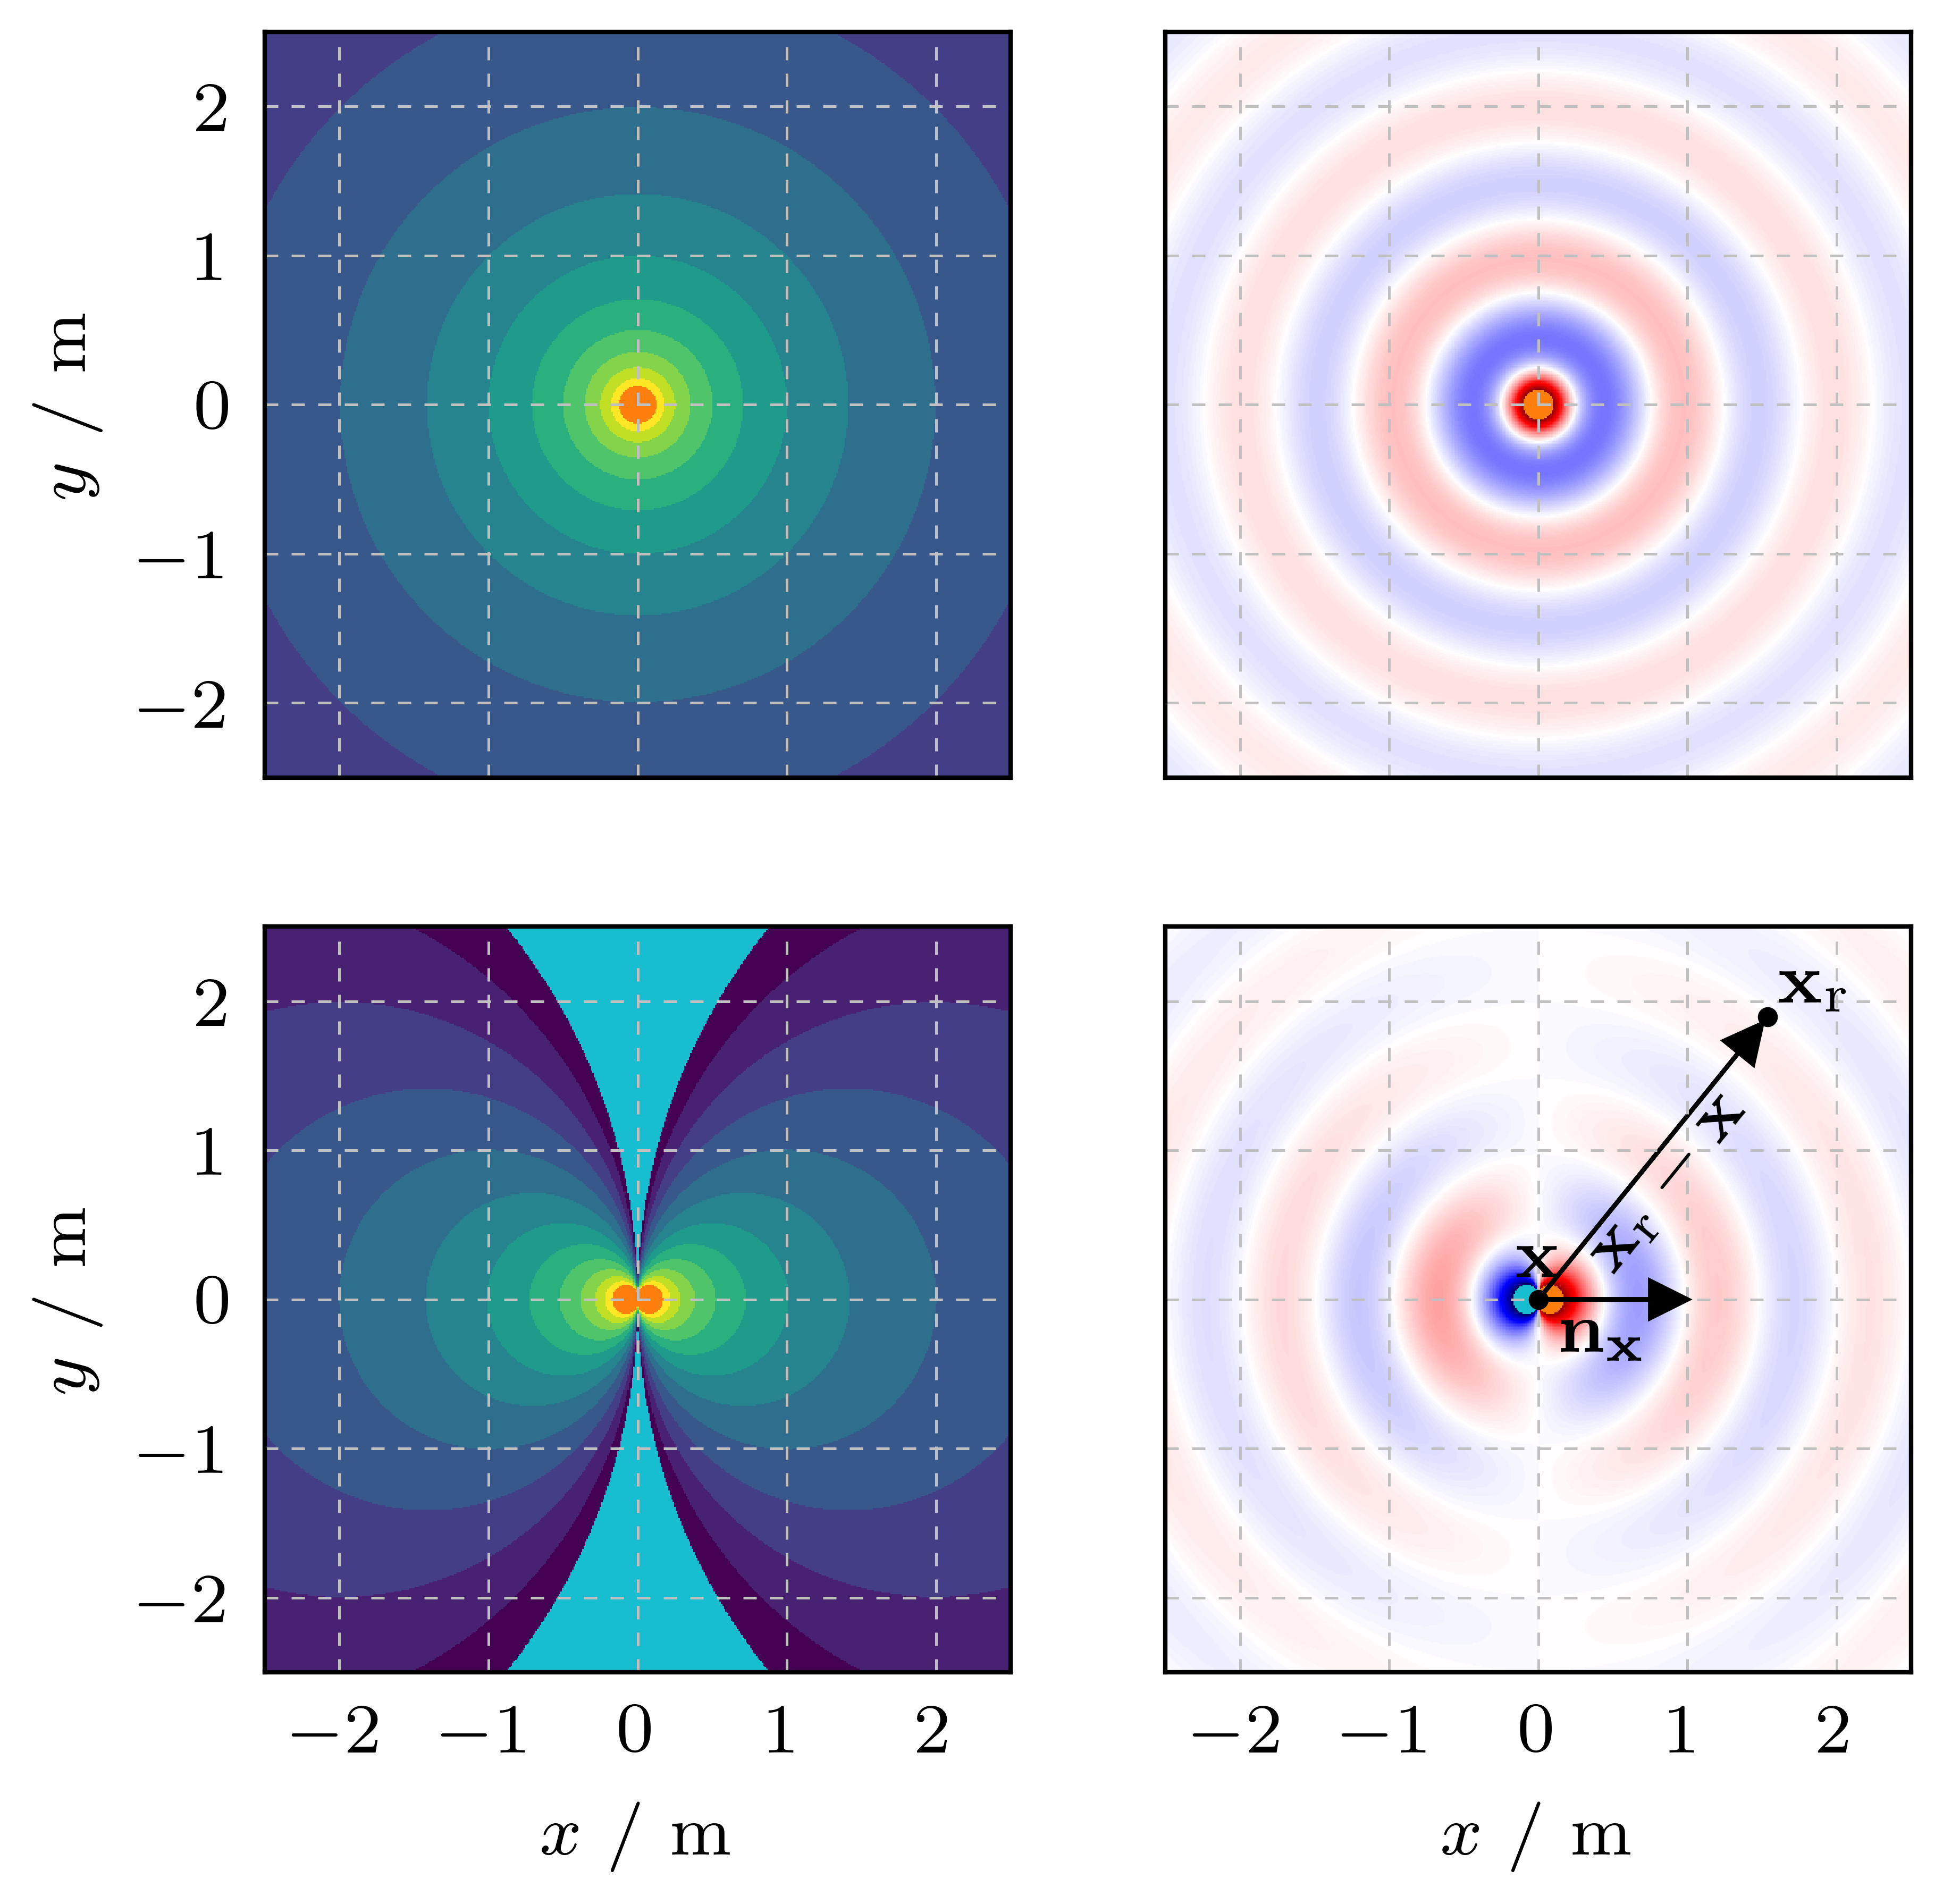
\includegraphics[width=85mm]{../python/monopole_dipole.png}
\end{plotfigures}
\caption{Schallfeld in der $xy$-Ebene.
Oben: normalisierter Monopol $4 \pi G(r_{\xs\text{-}\xr})$,
unten: normalisierter Dipol $4 \pi \frac{c}{\omega} G_\text{Dipol}(r_{\xs\text{-}\xr})$.
Quellenposition $\xs=(0,0,0)^\mathrm{T}$\,m,
Wellenlänge $\lambda=1$ m, Schallgeschwindigkeit $c=343$\,m/s, visualisierter
Zeitpunkt $t=0$\,s,
%
Normalen-Richtungsvektor $\nx=(1,0,0)^\mathrm{T}$ zeigt in die Richtung der
positiven Dipol-Hauptkeule.
Farbskalierung gemäß \Abb\ref{fig:plot_colorbar}.
\cc
}
\label{fig:monopole_dipole}
\end{figure}



\Abb\ref{fig:plot_colorbar} referenziert die Farbskalen für den Pegel und
den instantanen, linearen Schalldruckwert,
welche jeweils bei allen dargestellten monofrequenten Schallfeldern benutzt
werden.
%
Ein monofrequentes Schallfeld des Monopols ist in
\Abb\ref{fig:monopole_dipole}~(oben) für die $xy$-Ebene visualisiert.
%
Das omnidirektionale Abstrahlverhalten des Monopols mit $6$\,dB-Pegelabnahme pro
Entfernungsverdopplung ist ersichtlich.

Der Dipol an der Position $\xs$ erzeugt ein monofrequentes Schallfeld, welches
sich auch aus der \Glg\eqref{eq:G03D} berechnen lässt.
%
Es ergibt sich aus deren räumlicher Ableitung
(Gradientenbildung bezüglich $\xs$ mit dem Operator
$\nabla = (\frac{\partial}{\partial x},\frac{\partial}{\partial y},\frac{\partial}{\partial z})^\mathrm{T}$
für kartesische Koordinaten)
und anschließender Projektion (Skalarprodukt) auf den gewünschten
Normalenvektor $\nx$
%
\begin{align}
\label{eq:G03D_Dipol}
G_\text{Dipol}(r_{\xs\text{-}\xr}) &=
\nxT \, \nabla G(r_{\xs\text{-}\xr}) \nonumber\\
&= -\nxT\,\bm{\theta}_{\xs\text{-}\xr}\cdot
G(r_{\xs\text{-}\xr}) \cdot \left(\im\wc +\frac{1}{r_{\xs\text{-}\xr}}\right).
\end{align}
%
Das Skalarprodukt der Vektoren $\bm{n}$ und $\bm{\theta}$ in
kartesischer Form wird als $\bm{n}^\mathrm{T} \bm{\theta}$ notiert.
%
Der Einheitsvektor
\begin{align}
\bm{\theta}_{\xs\text{-}\xr} :=
\frac{\xs-\xr}{\|\xs-\xr\|}  =
\frac{\xs-\xr}{r_{\xs\text{-}\xr}}
\end{align}
zeigt vom Messpunkt $\xr$ zur Dipol- bzw. Monopolposition $\xs$.
%
Für hohe Frequenzen und/oder weit entfernte Abstände
$\frac{\omega}{c} r_{\xs\text{-}\xr} \gg 1$ kann Glg.\,\eqref{eq:G03D_Dipol}
mit
\begin{align}
\label{eq:DipolHF}
G_\text{Dipol}(r_{\xs\text{-}\xr}) \approx
-\nxT\,\bm{\theta}_{\xs\text{-}\xr}\,
G(r_{\xs\text{-}\xr}) \, \im\wc
\end{align}
%$G_\text{Dipol}(r_{\xs\text{-}\xr}) \approx
%-\nxT\,\bm{\theta}_{\xs\text{-}\xr}\,
%G(r_{\xs\text{-}\xr}) \, \im\wc$
genähert werden.
%
In \Abb\ref{fig:monopole_dipole}~(unten) ist beispielhaft das Schallfeld
eines Dipols visualisiert.
%
Der Normalenvektor $\nx$ in Richtung der $x$-Achse zeigt in Richtung der
zu $t=0$\,s positiven Dipol-Hauptkeule\index{Hauptkeule}.
%
Dies ergibt inhärent die dazu 90$^\circ$ stehende $yz$-Ebene, in welcher der
Schalldruck beim Dipol Null ist (Dipolnullstelle).
%
Beachtenswert ist die exakte $90^\circ$-Phasenverschiebung zwischen Monopol und
hochfrequenzgenähertem Dipol.



\subsection{Kirchhoff-Helmholtz-Hüllflächenintegral}
%
Nun sei ein Volumen $V$ durch eine Hüllfläche $S$ umschlossen, wie es
in \Abb\ref{fig:KHIGeometrie} mit dem blauen Körper angedeutet ist.
%
Auf die Hüllfläche werden mit infinitesimalem Abstand
Monopole und Dipole als sogenannte Sekundärquellen\index{Sekundärquelle}
platziert.
%
Jedem Punkt $\xs$ auf der Hüllfläche ist ein senkrecht zur Fläche,
aus dem Volumen herauszeigender Normalenvektor $\nx$ zugewiesen.
%
% please DO NOT rescale the figure and keep it single column
\begin{figure}[t]
\centering
\begin{plotfigures}
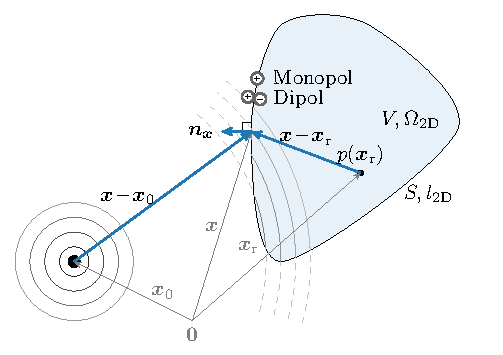
\includegraphics[width=85mm]{../graphics_DEU/khi_geometry.pdf}
\end{plotfigures}
\caption{Geometrie für das Kirchhoff-Helmholtz-Integral (KHI)
in \Glg\eqref{eq:KHIGeneral} zur
Schalldrucksynthese innerhalb eines quellenfreien Volumens $V$.
%
Positionen $\xs$ von Mono- und Dipolen (Sekundärquellen) auf der Hüllfläche
$S$ mit herauszeigendem Normalenvektor $\nx$,
%
Position $\xp$ der virtuellen Punktquelle (Primärquelle),
%
Empfänger-/Mess-/Aufpunkt(e) $\xr$.
%
In der Praxis wird oft monopolbasierte Schalldrucksynthese mit einer konvexen
Hüllkontur $l_\text{2D}$ realisiert, welche die Fläche $\Omega_\text{2D}$ in einer
gewählten Zuhörerebene einschließt.
%
\cc
}
\label{fig:KHIGeometrie}
\end{figure}
%
Die exakte und eindeutige Synthese des Schalldrucks $p(\xr)$ wird als
Schallfeldüberlagerung gewichteter Mono- und Dipole durch das
als Kirchhoff-Helmholtz-Integral\index{Kirchhoff-Helmholtz-Integral} (KHI)
bekannte Hüllflächenintegral, vgl. \cite[Kap.~23.2]{Skudrzyk1971}
%
\begin{align} %underbrace sortiert
\label{eq:KHIGeneral}
p(\xr) = \int\limits_S
%\left(
[
&\underbrace{\nxT \, \nabla p(\xs)}_{\text{Monopolsignal}}\cdot
\underbrace{G(r_{\xs\text{-}\xr})}_{\text{Monopol}}
-\nonumber\\
&\underbrace{p(\xs)}_{\text{Dipolsignal}} \cdot
\underbrace{\nxT \, \nabla G(r_{\xs\text{-}\xr})}_{\text{Dipol}}
]
%\right)
\,\mathrm{d}S,
\end{align}
%
für Empfängerpunkte $\xr$ innerhalb eines quellenfreien Volumens $V$ beschrieben;
%
für $\xr$ außerhalb $V$ gilt dann $p(\xr)=0$.
%
Das KHI in \Glg\eqref{eq:KHIGeneral} ist die fundamentale, integrale
Beschreibung des Phänomens lineare Wellenausbreitung und -überlagerung.
%
Es ist die Grundlage für Schallfeldsynthese im Allgemeinen, speziell also auch
für die WFS.
%
In der Praxis wird das Schallfeld durch die
Überlagerung von sich ausbreitenden Schallfeldern der individuell angesteuerten
Lautsprecher erzeugt, und somit $p(\xr)$ über eine diskrete Summation erzeugt.
%
Die resultierende, physikalisch begründete Approximation des eigentlich
intendierten Schallfeldes ist charakteristisch für alle KHI-basierten
Schallfeldsyntheseverfahren, daher nicht WFS-spezifisch.
%
Der Schalldruckverlauf über die Zeit wird mit $\Re\{p(\xr)\cdot\e^{+\im \omega t}\}$
für ein monofrequentes Schallfeld mit der Kreisfrequenz $\omega$
berechnet.



\subsection{Gewichtungssignale für daten- und modellbasierten WFS-Ansatz}
%
Mit der WFS können Schallszenarien, oft auch akustische
Szenen genannt, bestehend aus räumlich und zeitlich gestaffelten Wellenfronten
synthetisiert werden.
%
Im WFS-Kontext gibt es zwei grundständige Herangehensweisen zur Erzeugung von
akustischen Szenen: die datenbasierte und die modellbasierte.
%
Die datenbasierte WFS, vgl. \cite{Berkhout1988_JAES}
verarbeitet direkt akustische Messungen als WFS-Ansteuerungssignale,
wie in \Abb\ref{fig:violine} angedeutet.
%
Die modellbasierte WFS, vgl. \cite{Berkhout1993_JASA}
arbeitet mit Modellen für virtuelle Schallquellen wie in
\Abb\ref{fig:KHIGeometrie} skizziert.
%
Dieser Ansatz ist Bestandteil von objektbasierter Wiedergabe
\cite{Vaananen2002, Plogsties2003, Plogsties2003, Brandenburg2004, Geier2008,Spors2013_IEEE,Sporer2018_book},
für die Audiosignal, Modelltyp und -parametrik einem, mit der WFS zu
spatialisierenden, Audio-Objekt zugewiesen werden.



Die Gewichtungssignale $\nxT \, \nabla p(\xs)$ für die Monopole im KHI
(in \Glg\eqref{eq:KHIGeneral} als Monopolsignal bezeichnet)
sind die normalen-projizierten Schalldruckgradienten auf der Hüllfläche.
%
Diese Signale sind proportional zur normalen Schallschnelle bezüglich der Hüllfläche,
vgl. \cite{Berkhout1993_JASA, Vries1996_JAES}.
%
Beim datenbasierten Direkt-Wiedergabeansatz stammen sie von
Messungen bzw. von Aufnahmen mit Druckgradientenmikrofonen
mit Achter-Richtcharakteristik, wobei die Hauptkeule
orthogonal zur Hüllfläche ausgerichtet ist, vgl.~\Abb\ref{fig:violine}.
%
Die Gewichtungssignale $p(\xs)$ für die Dipole im KHI (in
\Glg\eqref{eq:KHIGeneral} als Dipolsignal bezeichnet)
entsprechen den Schalldrücken auf der Hüllfläche.
%
Diese können für den datenbasierten Ansatz direkt mit omnidirektionalen
Druckempfängern aufgezeichnet werden.
%
Die datenbasierte Direktwiedergabe entspricht im Wesen der Utopie
von \cite{Fletcher1934,Steinberg1934} ohne weitere
Signalaufbereitung zwischen \textit{screen of microphones} und
\textit{screen of loudspeakers} \cite[S.\,572]{Snow1953}.
%
Die Manipulationsmöglichkeiten räumlicher und zeitlicher Parameter beim
datenbasierten Ansatz mit Zwischenverarbeitung der Mikrofonsignale sind
eingeschränkt, dafür kann die räumlich-zeitliche Komplexität eines
Schallfeldes durch geeignete Messauflösung vergleichsweise
einfach erfasst und synthetisiert
werden, vgl. \cite{Sonke2000_diss,Hulsebos2004_diss,Vries2007_JASP}.



Beim modellbasierten Ansatz errechnen sich die benötigten Gewichtungssignale
$\nxT \, \nabla p(\xs)$ und $p(\xs)$ aus dem Schallfeld eines analytisch
gegebenen Quellenmodells -- z.B. eine außerhalb von $V$ befindliche Punktquelle,
wie jene bei $\xp$ in \Abb\ref{fig:KHIGeometrie} -- dem ein zu spatialisierendes
Audiosignal aufgeprägt wird.
%
Ein Quellenmodell wird im WFS-Kontext oft als virtuelle Quelle oder als
Primärquelle\index{Primärquelle} bezeichnet.
%
Die auf der Hüllfläche $S$ positionierten Mono- und Dipole werden hingegen
als Sekundärquellen\index{Sekundärquelle} bezeichnet.
%
Beim modellbasierten Wiedergabeansatz
werden typischerweise einfache Quellenmodelle gewählt, einhergehend mit vergleichsweise
geringer Schallfeldkomplexität, dafür aber mit einfacher Variationsmöglichkeit
der Raum-Zeit-Parametrik des Quellenmodells.
%
Einfache virtuelle Quellenmodelle sind die
Punktquelle \cite{Berkhout1993_JASA,Start1997_diss},
die sogenannte fokussierte Punktquelle \cite{Verheijen1997_diss,Spors2007b,Melchior2008,Wierstorf2014_diss}
und die ebene Welle \cite{Spors2008a, Voelk2012, Firtha2019_diss}.
%
Das ebene Wellenmodell kann als Grenzfall der sehr weit
entfernten Punktquelle aufgefasst werden.
%
Für die Punktquelle wurden Modellerweiterungen für Quellrichtcharakteristika und
Bewegungstrajektorien diskutiert, vgl. \cite{Corteel2007_JASP,Baalman2008_diss,Franck2012,Romoli2015_ApplAc,Schultz2017,Franck2007,Ahrens2011,Firtha2019_diss}.



Beiden Ansätzen, dem daten- bzw. dem modellbasierten, ist ein gemessener bzw.
ein gewünschter, analytisch bekannter Wellenfrontverlauf gemein, der auf Basis
des KHIs rekonstruiert bzw. synthetisiert werden soll.
%
Daraus resultieren die in der Literatur synonym verwendeten Begriffe
Wellenfrontsynthese\index{Wellenfrontsynthese} und
Wellenfeldsynthese \cite{Berkhout1992b,Berkhout1992a}.



\section{Modellbasierter Ansatz für die WFS einer virtuellen Punktquelle}
\label{sec:WFS_PointSource}
%
Weil die virtuelle Punktquelle ein fundamentales Quellenmodell darstellt und in
der WFS-Produktionspraxis eine wichtige Rolle spielt, soll im Folgenden
auf die modellbasierte WFS der virtuellen Punktquelle näher eingegangen werden.
%
Diese soll bei $\xp$ außerhalb von $V$ positioniert sein\footnote{Die sogenannte
fokussierte Quelle erhält man, wenn $\xp$ innerhalb von $V$ zugelassen wird,
was hier zu Gunsten anderer Inhalte nicht im Detail diskutiert wird.},
vgl.~\Abb\ref{fig:KHIGeometrie}.
%
Damit definiert sich der Einheitsvektor
\begin{align}
\bm{\theta}_{\xs\text{-}\xp} :=
\frac{\xs-\xp}{\|\xs-\xp\|} =
\frac{\xs-\xp}{r_{\xs\text{-}\xp}}
\end{align}
von der virtuellen Punktquelle $\xp$ zu einem Hüllflächenpunkt
$\xs$ zeigend.
%
Der Abstand zwischen diesen beiden Punkten ist
$r_{\xs\text{-}\xp}=\|\xs-\xp\|$.



\subsection{Fernfeld-/Hochfrequenz-Näherung des KHI}
%
Die virtuelle Punktquelle mit komplexer Amplitude $A$ erzeugt auf der Hüllfläche $S$
das monofrequente Schallfeld
$p(\xs) = A \cdot G(r_{\xs\text{-}\xp})$.
%
Für die Synthese einer Wellenfront ausgehend von dieser virtuellen Punktquelle
wird $p(\xs)$ in das KHI in \Glg\eqref{eq:KHIGeneral} eingesetzt.
%
Unter den Bedingungen
$\wc r_{\xs\text{-}\xr} \gg 1$ und
$\wc r_{\xs\text{-}\xp} \gg 1$
kann der Integrand genähert werden (vgl.~\Glg\eqref{eq:G03D_Dipol} und
\eqref{eq:DipolHF}), was zum Schallfeld $p(\xr)$
%
\begin{align}
%\label{eq:KHIFarMono}
p(\xr) \approx \int\limits_S [
&\underbrace{-A\,
\im\wc\,
\nxT \bm{\theta}_{\xs\text{-}\xp}\,
G(r_{\xs\text{-}\xp})}_{\text{Monopolsignal, hochfrequenzgenähert}}
%
\cdot \underbrace{G(r_{\xs\text{-}\xr})}_{\text{Monopol}}-
\nonumber\\
&\underbrace{A \, G(r_{\xs\text{-}\xp})}_{\text{Dipolsignal}}
\cdot
\underbrace{(-\im\wc)\,
\nxT \bm{\theta}_{\xs\text{-}\xr}\,
G(r_{\xs\text{-}\xr})}_{\text{Dipol, hochfrequenzgenähert, vgl.~\eqref{eq:DipolHF}}}
%
]\,\mathrm{d}S
\end{align}
%
führt und die Grundlage zur Beschreibung
der in Seismik, Optik und Akustik bekannten Fresnel-Kirchhoff-Beugung einer
Punktquelle darstellt, sowie Ausgangspunkt der
High Frequency Boundary Element Method
(HF-BEM) ist, vgl. \cite{Schultz2016_diss, Zotter2013, Firtha2019_diss}.
%
Diese auch für WFS verwendeten Fernfeld- und/oder
Hochfrequenznäherungen
\index{Fernfeld-/Hochfrequenznäherung}
\index{Hochfrequenz-/Fernfeldnäherung}
fordern, dass die jeweiligen Abstände
%\begin{align}
%r_{\xs\text{-}\xp}=\|\xs-\xp\|\qquad
%r_{\xs\text{-}\xr}=\|\xs-\xr\|
%\end{align}
$r_{\xs\text{-}\xp}=\|\xs-\xp\|$ (virtuelle Quelle zu Sekundärquelle) und
$r_{\xs\text{-}\xr}=\|\xs-\xr\|$ (Sekundärquelle zu Empfänger)
%
deutlich größer sind als die betrachtete Wellenlänge
$\lambda = 2\pi\frac{c}{\omega}$.
%
Das Integral kann umgeschrieben werden zu
%
\begin{align}
\label{eq:KHIFarMono}
p(\xr) \approx \int\limits_S A \cdot
&\underbrace{\im\wc \cdot \nxT\left(\bm{\theta}_{\xs\text{-}\xr} - \bm{\theta}_{\xs\text{-}\xp}\right)
\cdot G(r_{\xs\text{-}\xp})}_{\substack{\text{Grundlage für Ansteuerung } D(\xp,\xs) \text{,} \\ \text{Dipol Abhängigkeit}}}
\times\nonumber\\
&\underbrace{G(r_{\xs\text{-}\xr})}_{\text{Monopol}}
\mathrm{d}S,
\end{align}
%
%
wobei beachtenswert ist, dass trotz der Freistellung des
Monopolquelltyps in \Glg\eqref{eq:KHIFarMono} hochfrequenzgenäherte
Sekundär-Dipole mit dem Term $\im\wc\,\nxT\,\bm{\theta}_{\xs\text{-}\xr}\,
G(r_{\xs\text{-}\xr})$ enthalten sind, vgl.~\eqref{eq:DipolHF}.



\subsection{Monopolbasierte 3D- und 2.5D-Syntheseintegrale}
%
Um den praktischen Aufwand maßvoll zu gestalten, wird bei der Realisierung von WFS
typischerweise nur ein Lautsprechertyp für die Sekundärquellen verwendet,
vgl. \cite{Vries1996_JAES}.
%
Diese Einschränkung für das KHI hat zur Folge,
dass auch ein Schallfeld außerhalb des Synthesevolumens
erzeugt wird, welches einen etwaigen Wiedergaberaum anregt,
vgl. \cite{Start1997_diss, Wittek2007_JAES, Wittek2007_diss, Gauthier2007_Acta,Erbes2020_diss},
und das gewünschte Schallfeld von Raumreflexionen überlagert wird.
%
Typische Lautsprecherboxen verhalten sich im tieffrequenten, für WFS praktikablen
Frequenzbereich (vgl.~\Glg\eqref{eq:SamplingCriterion})
annähernd monopolartig und weisen mit zunehmender Frequenz
eine zunehmende Richtwirkung zur Frontalrichtung hin auf.
%
Die weitere Betrachtung erfolgt daher vereinfachend mit Monopolen und
ohne Berücksichtigung von Raumeinflüssen, d.h. für Freifeldbedingungen.



Das Integral für 3D-Synthese\index{3D-Synthese} mit Monopolen auf der Hüllfläche $S$
kann allgemeiner
\begin{align}
p(\xr) =& \int\limits_S A \, D_\text{3D}(\xp,\xs) \, G(r_{\xs\text{-}\xr}) \, \mathrm{d}S
\label{eq:MonopolIntegral_3D}
\end{align}
geschrieben werden.
Die unbekannte, sogenannte Treiberfunktion $D_\text{3D}(\xp,\xs)$
stellt eine lautsprecherindividuelle, komplexe Gewichtung der
Eingangssignalamplitude $A$ der virtuellen Punktquelle dar.
%
Das komplexe Gewicht geht bei breitbandiger Betrachtung in das Spektrum
$D_\text{3D}(\xp,\xs,\omega)$ über.
Dieses wird im Folgenden Filter-Frequenzgang genannt, um es eindeutig
vom Frequenzgang eines breitbandigen Schallfeldes, welcher an einem
bestimmten Empfängerpunkt gemessen wird, unterscheidbar zu machen.
%
Breitbandig ergibt sich im Frequenzbereich somit die Multiplikation des
Audio-Eingangssignalspektrums $A(\omega)$ der virtuellen Quelle
mit dem lautsprecherindividuellen Filter-Frequenzgang
$D_\text{3D}(\xp,\xs,\omega)$ der gesuchten WFS-Ansteuerung.



Um den praktischen Aufwand weiter zu reduzieren, wird statt
einer Hüllfläche $S$ eine Hüllkontur $l_\text{2D}$ verwendet.
%
Für die WFS innerhalb einer Horizontalebene kommen dabei oft lineare bzw.
kreis- oder rechteckartig umhüllende Lautsprecherarrays zum Einsatz,
idealerweise auf Ohrhöhe,
vgl.~\Abb\ref{fig:WFS_Array_Haus8}, \cite{Vries2009_Mono,Vries2019}.
%
Das Syntheseintegral mit Monopolen auf der Hüllkontur $l_\text{2D}$
lautet allgemein
\begin{align}
p(\xr) =& \int\limits_{l_\text{2D}} A \, D_\text{2.5D}(\xp,\xs,\xr) \, G(r_{\xs\text{-}\xr}) \, \mathrm{d}l_\text{2D}.
\label{eq:MonopolIntegral_25D}
\end{align}
%
Für diesen Fall wird typisch und praxisrelevant angenommen, dass
virtuelle Quelle, Hüllkontur und Empfängerpunkte in der gleichen Ebene liegen.
%
Das Linienintegral und die betrachtete Syntheseebene sind zwei-dimensional,
der gewählte Primär- und Sekundärquellentyp Monopol erzeugt hingegen ein
drei-dimensionales Schallfeld.
%
Die Synthese mit \Glg\eqref{eq:MonopolIntegral_25D} liefert nun daher
zwar ein 3D-Schallfeld, welches aber nur von zwei ortsspezifischen
Variablen abhängig ist und
entsprechend nur in 2D kontrolliert bzw. parametrisiert werden kann.
%
Dies ist in der Wellentheorie bekannt als zweieinhalb-dimensionales
Problem \cite{Bleistein1986}. %,Bleistein2001}.
%
Die zugeschnittene, gesuchte Treiberfunktion $D_\text{2.5D}(\xp,\xs,\xr)$ bzw.
der Filter-Frequenzgang $D_\text{2.5D}(\xp,\xs,\xr,\omega)$ erhalten daher
den Index \text{2.5D}, um die zweieinhalb-dimensionale WFS, also
die 2.5D-Synthese\index{2.5D-Synthese}, klar vom 3D-WFS-Fall abzugrenzen.


Die Integrale in den \Glgn\eqref{eq:MonopolIntegral_3D}, \eqref{eq:MonopolIntegral_25D}
stellen Faltungen bezüglich der Ortsvariablen dar.
%
Sie sind selten geschlossen analytisch berechenbar.
%
Die gesuchte Treiberfunktion / der Filter-Frequenzgang $D_{\cdot\text{D}}$
ist Teil des Integranden.
%
Drei wesentliche Verfahren zum Lösen nach der Treiberfunktion sind möglich:
%
a) numerische Lösungen aus einem diskretisierten, inversen
Problem, vgl. \cite{Ise1999,Kolundzija2009a,Bai2015_JASA,Koyama2020_IEEE}
b) explizite analytische Lösungen für einfache Geometrien als räumliches
Entfaltungsproblem \cite{Ahrens2008_Acta,Spors2010a,Ahrens2010_IEEE,Fazi2010,Koyama2013}
und c) die implizite analytische Lösung, bei dem die Ansteuerungsfilter
aus dem Integranden der Hochfrequenznäherung in \Glg\eqref{eq:KHIFarMono}
extrahiert werden können.
%
Für Audioanwendungen wurde letztgenannte Methode als WFS in \cite{Berkhout1993_JASA, Vries1996_JAES}
für die planare bzw. die lineare Sekundärquellengeometrie
unter Benutzung der sogenannten Rayleigh-Integrale \cite[Kap.~25.5]{Skudrzyk1971}
eingeführt und in Folge in
\cite{Start1997_diss,Verheijen1997_diss,Voelk2012,Zotter2013,Firtha2019_diss,ZotterSchultz2020_White}
konsolidierend ausformuliert.
%
Die theoretische Abhandlung \cite{Firtha2019_diss} für die WFS von
allgemeinen konvexen, divergierenden Wellenfronten inklusive physikalisch korrekter
Abbildung bewegter Quellen liefert eine stringente Analyse lokaler
Wellenfrontkrümmungen und Wellenrichtungsvektoren für verschiedene
Schallfeldsyntheseintegrale.
%
Mit dieser Sichtweise können die bekannten WFS-Lösungen konsistent verortet und
z.B. für bewegte Quellen \cite{Franck2007, Ahrens2011} erweitert werden.
%
Basierend auf \cite{ZotterSchultz2020_White} soll
eine diesem Kapitel angemessen kompakte, verallgemeinernde Betrachtung
weiterverfolgt werden.



\subsection{WFS als implizite Lösung mit Sattelpunktsnäherung}
%
Für die implizite Lösung nach der Treiberfunktion muss das Integral
in \Glg\eqref{eq:KHIFarMono} weiter vereinfacht werden.
%
Vor allem muss für die intendierte monopolbasierte Synthese
der in \Glg\eqref{eq:KHIFarMono} noch vorhandene Sekundärquellentyp Dipol
eliminiert werden.
%
Die Vereinfachung gelingt mit der sogenannten Sattelpunktsnäherung
\index{Sattelpunktsnäherung}
(\textit{stationary phase approximation}), welche
die Hochfrequenznäherung voraussetzt.
%
Die Sattelpunktsnäherung liefert den Schalldruck für \textit{einen} beliebigen
Empfängerpunkt $\xr$ im Zuhörerbereich für 3D-Synthese
%
\begin{align}
\label{eq:pStat3D}
p(\xr) \approx A \cdot G(r_{\xr\text{-}\xp})
\end{align}
%
und für 2.5D-Synthese
%
\begin{align}
\label{eq:pStat25D}
p(\xr) \approx A\cdot
\sqrt{\frac{\frac{\im \omega}{c}}{2\pi}}\sqrt{\frac{r_{\xs\text{-}\xr} + r_{\xs\text{-}\xp}}{r_{\xs\text{-}\xr} \cdot r_{\xs\text{-}\xp}}}\cdot G(r_{\xr\text{-}\xp}).
\end{align}
%
Das komplexe Gewicht $G(r_{\xr\text{-}\xp})$ beschreibt die Schallausbreitung
einer Punktquelle
bei $\xp$ zum Empfängerpunkt $\xr$ mit dem Abstand $r_{\xr\text{-}\xp} = \|\xr-\xp\|$, vgl.~\eqref{eq:G03D}.
%
Die Näherung beinhaltet also die gewünschte lokale Phase des zu synthetisierenden
Schallfeldes am Empfängerpunkt.
%
Im 3D-Fall ist Amplitude und Phase inhärent korrekt und führt
exakt zum gewünschten komplexen Wert des Schalldrucks der virtuellen Punktquelle.
%
Im 2.5D-Fall hingegen weicht der gewünschte Schalldruck gemäß der zwei Wurzel-Ausdrücke
in \Glg\eqref{eq:pStat25D} ab.



Aus der Sattelpunktsnäherung lässt sich zudem schliessen,
dass dieses lokal begrenzte Ergebnis
maßgeblich von nur \textit{einem} Sekundärmonopol auf der Hüllfläche/-linie
erzeugt wird.
%
Er befindet sich an der Position $\xs$, wo der Direktpfad von virtueller
Quelle $\xp$ zu Empfängerpunkt $\xr$ die Hülle durchstößt,
vgl.~\Abb\ref{fig:3DWFS_Schema} und \ref{fig:25DWFS_Schema}.
Dieses $\bm{x}$ ist für das Integral in \Glg\eqref{eq:KHIFarMono} ein
Punkt stationärer Phase, der so genannt wird,
weil in dessen Umgebung der Phasenterm des Integranden am wenigsten oszilliert.
%
Genau dann gilt $\bm{\theta}_{\xs\text{-}\xr} = -\bm{\theta}_{\xs\text{-}\xp}$
und damit für den Term in \Glg\eqref{eq:KHIFarMono} die Beziehung
$\nxT \, \left(\bm{\theta}_{\xs\text{-}\xr} - \bm{\theta}_{\xs\text{-}\xp}\right)
= - 2 \nxT \, \bm{\theta}_{\xs\text{-}\xp}$.
%
Dadurch vereinfacht sich das Integral, weil keine sekundären Dipolquellen mehr zur
Synthese benötigt werden.
% 3D-WFS
% please DO NOT rescale the figure and keep it single column
\begin{figure}[t]
\centering
\begin{plotfigures}
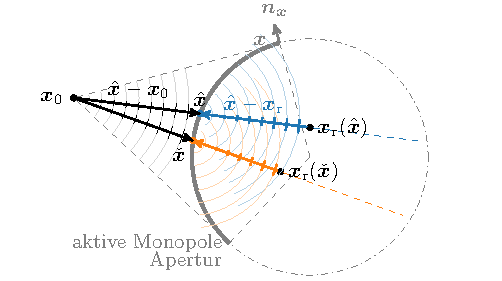
\includegraphics[width=85mm]{../graphics_DEU/spa_3d.pdf}
\end{plotfigures}
\caption{3D-WFS.
%
Monopole bei $\xs$, angeordnet zu einem kugelförmigen Array, und eine
virtuelle Punktquelle bei $\xp$.
%
Die Sattelpunktsnäherung kann als akustisches Strahlenmodell interpretiert werden:
%
nur der auf dem Direktpfad von virtueller Quelle zu Empfänger (Vektor $\xr - \xp$)
auf der Hüllfläche liegende Monopol trägt maßgeblich zur
Synthese des Schallfelds der virtuellen Quelle bei.
%
Für alle Punkte auf der Direktpfadverlängerung
(beispielhaft ausgehend von $\hat{\bm{x}}$ entlang blau bzw. von $\check{\bm{x}}$
entlang orange) ist die Synthese bei 3D-WFS amplitudenkorrekt.
%
Darstellung hier in 2D, man stelle sich eine Kugelkappe als
Geometrie der aktiven Sekundärquellen vor, Empfängerpunkte innerhalb der Kugel.
%
\cc
}
\label{fig:3DWFS_Schema}
\end{figure}
% 2.5D-WFS
% please DO NOT rescale the figure and keep it single column
\begin{figure}[t]
\centering
\begin{plotfigures}
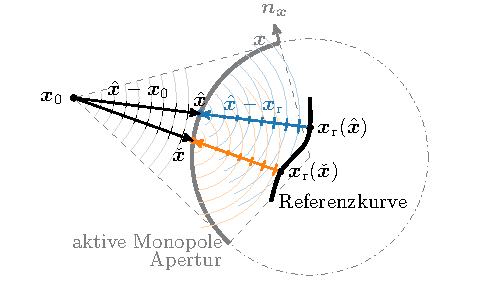
\includegraphics[width=85mm]{../graphics_DEU/spa_25d.pdf}
\end{plotfigures}
\caption{2.5D-WFS. Alle Punkte und Vektoren in der gleichen Ebene.
%
Monopole bei $\xs$, angeordnet zu einem kreisförmigen Array, und eine
virtuelle Punktquelle bei $\xp$.
%
Sattelpunktsnäherung für 2.5D-WFS:
entlang des in den Zuhörerbereich verlängerten Pfades $\xs - \xp$ trägt nur der
Monopol am Hüllkontur-Durchstoßpunkt maßgeblich zum synthetisierten
Schallfeld bei.
%
Amplitudenkorrekte Synthese ist für genau einen Referenzpunkt
$\xr(\xs)$ auf diesem Pfad möglich.
%
Umkehrschluss: Entlang einer in Grenzen wählbaren Referenzkurve mit den Punkten
$\xr(\xs)$ -- in der Grafik angedeutet mit
$\xr(\hat{\bm{x}})$ bzw. $\xr(\check{\bm{x}})$
für die Monopole bei $\hat{\bm{x}}$ bzw.
$\check{\bm{x}}$ -- findet sich für jeden Referenzpunkt genau eine Quelle $\xs$
auf dem Pfad von virtueller Quelle zu Referenzpunkt.
%
Mittels Amplitudenkorrektur dieser Quelle $\xs$ (vgl.~\Glg\eqref{eq:Driving25D})
gelingt amplitudenkorrekte
Synthese entlang der gewählten Referenzkurve $\xr(\xs)$.
%
\cc
}
\label{fig:25DWFS_Schema}
\end{figure}
%
Beiträge zur Lösung mit potentiell anderen Punkten stationärer Phase
-- unbrauchbare Spiegelreflexionen \cite{ZotterSchultz2020_White} -- werden
formal mit der Maximum-Operation
\begin{align}
\label{eq:SecSrcSel}
2\cdot\mathrm{max}\{-\nxT \, \bm{\theta}_{\xs\text{-}\xp}, 0\}
\end{align}
unterdrückt.
Dieses sattelpunktsnäherung-inhärente Kriterium ist identisch mit dem sogenannten
\textit{secondary source selection criterion}
\index{secondary source selection criterion} \cite{Nicol1999, Spors2007b, Spors2008a},
welches bei WFS-Herleitungen gesondert eingeführt wurde.
%
Es ist auch im Kontext der HF-BEM bekannt und sorgt dafür,
dass bei der Synthese keine Monopole aktiv sind,
deren Wellenausbreitung in der Zuhörerfläche jener der virtuellen Quelle
entgegenlaufen.
%
In optischer Analogie sind nur die Monopole einer sinnvollerweise konvexen
Hüllfläche aktiv, von denen aus eine direkte Sicht auf die virtuelle Quelle
möglich ist, vgl.~\Abb\ref{fig:3DWFS_Schema}.



\subsection{WFS-Ansteuerung im Frequenzbereich}
%
Die Ergebnisse in \Glg\eqref{eq:pStat3D} und \eqref{eq:pStat25D} aus der
Sattelpunktsnäherung besagen, dass zur Erzeugung des Schalldrucks
an einem spezifizierten Punkt $\xr$ nur ein Monopol maßgeblich beteiligt ist,
was sich als Schallstrahlenmodell interpretieren lässt.
%
Da die Erzeugung des korrekten Schalldrucks für mehrere Empfängerpunkte im Fokus
der WFS steht, also mehrere Schallstrahlen zur korrekten Wellenfrontkrümmung
\index{Wellenfrontkrümmung}
beitragen sollen, müssen die \Glgn\eqref{eq:pStat3D}, \eqref{eq:pStat25D},
\eqref{eq:SecSrcSel} und
\eqref{eq:KHIFarMono} sinnvoll verknüpft werden, damit für die Syntheseintegrale
\eqref{eq:MonopolIntegral_3D}, \eqref{eq:MonopolIntegral_25D}
die benötigten WFS-Ansteuerungsfilter angegeben
werden können.
%
Dem impliziten Lösungsansatz folgend, wird dazu die erste
geschweifte Klammer in \Glg\eqref{eq:KHIFarMono} mit \eqref{eq:pStat3D} bzw.
\eqref{eq:pStat25D} verglichen.
%
Für eine breitbandige Ansteuerung resultiert der Filter-Frequenzgang
für den 3D-Synthese-Fall
%
\begin{align}
D_\text{3D}(\xp,\xs,\omega) = 2\im\wc \mathrm{max}\{-\nxT \, \bm{\theta}_{\xs\text{-}\xp}, 0\} \, G(r_{\xs\text{-}\xp},\omega)
\label{eq:Driving3D}
\end{align}
%
und der Filter-Frequenzgang für den 2.5D-Synthese-Fall, vgl. \cite{Deregowski1983,Bleistein1986}
%
\begin{align}
D_\text{2.5D}(\xp, \xs, \xr,\omega) = \underbrace{D_\text{3D}(\xp,\xs,\omega)}_{\text{3D-WFS Treiberfunktion \eqref{eq:Driving3D}}} \times\label{eq:Driving25D}\\
\underbrace{\sqrt{\frac{2\pi}{\im\wc} r_{\xs\text{-}\xr}}
\sqrt{\frac{r_{\xs\text{-}\xp}}{r_{\xs\text{-}\xr} + r_{\xs\text{-}\xp}}}}_{\text{reziproke Faktoren von \eqref{eq:pStat25D}}}\nonumber
\end{align}
%
für jeden Monopol $\xs$.
%
Bei 2.5D-Synthese sorgen die reziproken Wurzel-Faktoren
für die Kompensation der bei der Sattelpunktsnäherungslösung in \Glg\eqref{eq:pStat25D}
entstandenen Abweichung.
%
Der erste Wurzel-Ausdruck in \Glg\eqref{eq:Driving25D} ist ein Filter und
kompensiert den Umstand,
dass sich die 2D-Hüllkontur spektral anders verhält als die 3D-Hüllfläche,
während die zweite Wurzel als Gainwert die Amplitudenabnahme der 3D-Primärquelle
bezüglich der 2D-Zuhörerebene normalisiert, vgl. \cite[Kap.~4.1.3]{Firtha2019_diss}.
%
Letzteres wird im Folgenden als Amplitudenkorrektur bezeichnet.
%
Wenn $r_{\xs\text{-}\xp} \gg r_{\xs\text{-}\xr}$ eingehalten wird, weist die
synthetisierte Welle eine verschwindende Wellenkrümmung bei $\xr$ auf und
der zweite Wurzel-Ausdruck geht gegen Eins.
%
Dies kann für die 2.5D-WFS als ebenes Wellenmodell genutzt werden.



Die für 2.5D-WFS erforderliche Amplitudenkorrektur ist nur möglich für Punktpaare
stationärer Phase: Für ein bestimmtes $\xs$ kann ein bestimmtes $\xr$
festgelegt werden, für das die Synthese amplitudenkorrekt\index{amplitudenkorrekte Synthese}
sein soll, vgl.~\Abb\ref{fig:25DWFS_Schema}, \cite[Kap.~3]{Start1997_diss}, \cite[Kap.~4]{Firtha2019_diss}.
%
%Die gewählten $\xr$ sollten einen physikalisch sinnvollen Konturverlauf aufweisen,
%weil Schallstrahlen die eigentlich stattfindende Synthese stark vereinfacht
%modellieren und der freien Punktpaarwahl dadurch Grenzen gesetzt sind.
%
Der 3D-Fall ist amplitudenkorrekt für alle $\xr$, falls die oben eingeführten
Näherungsbedingungen eingehalten werden, vgl.~\Abb\ref{fig:3DWFS_Schema}.
%
% please DO NOT rescale the figure and keep it double column
\begin{figure*}[t]
\centering
\begin{plotfigures}
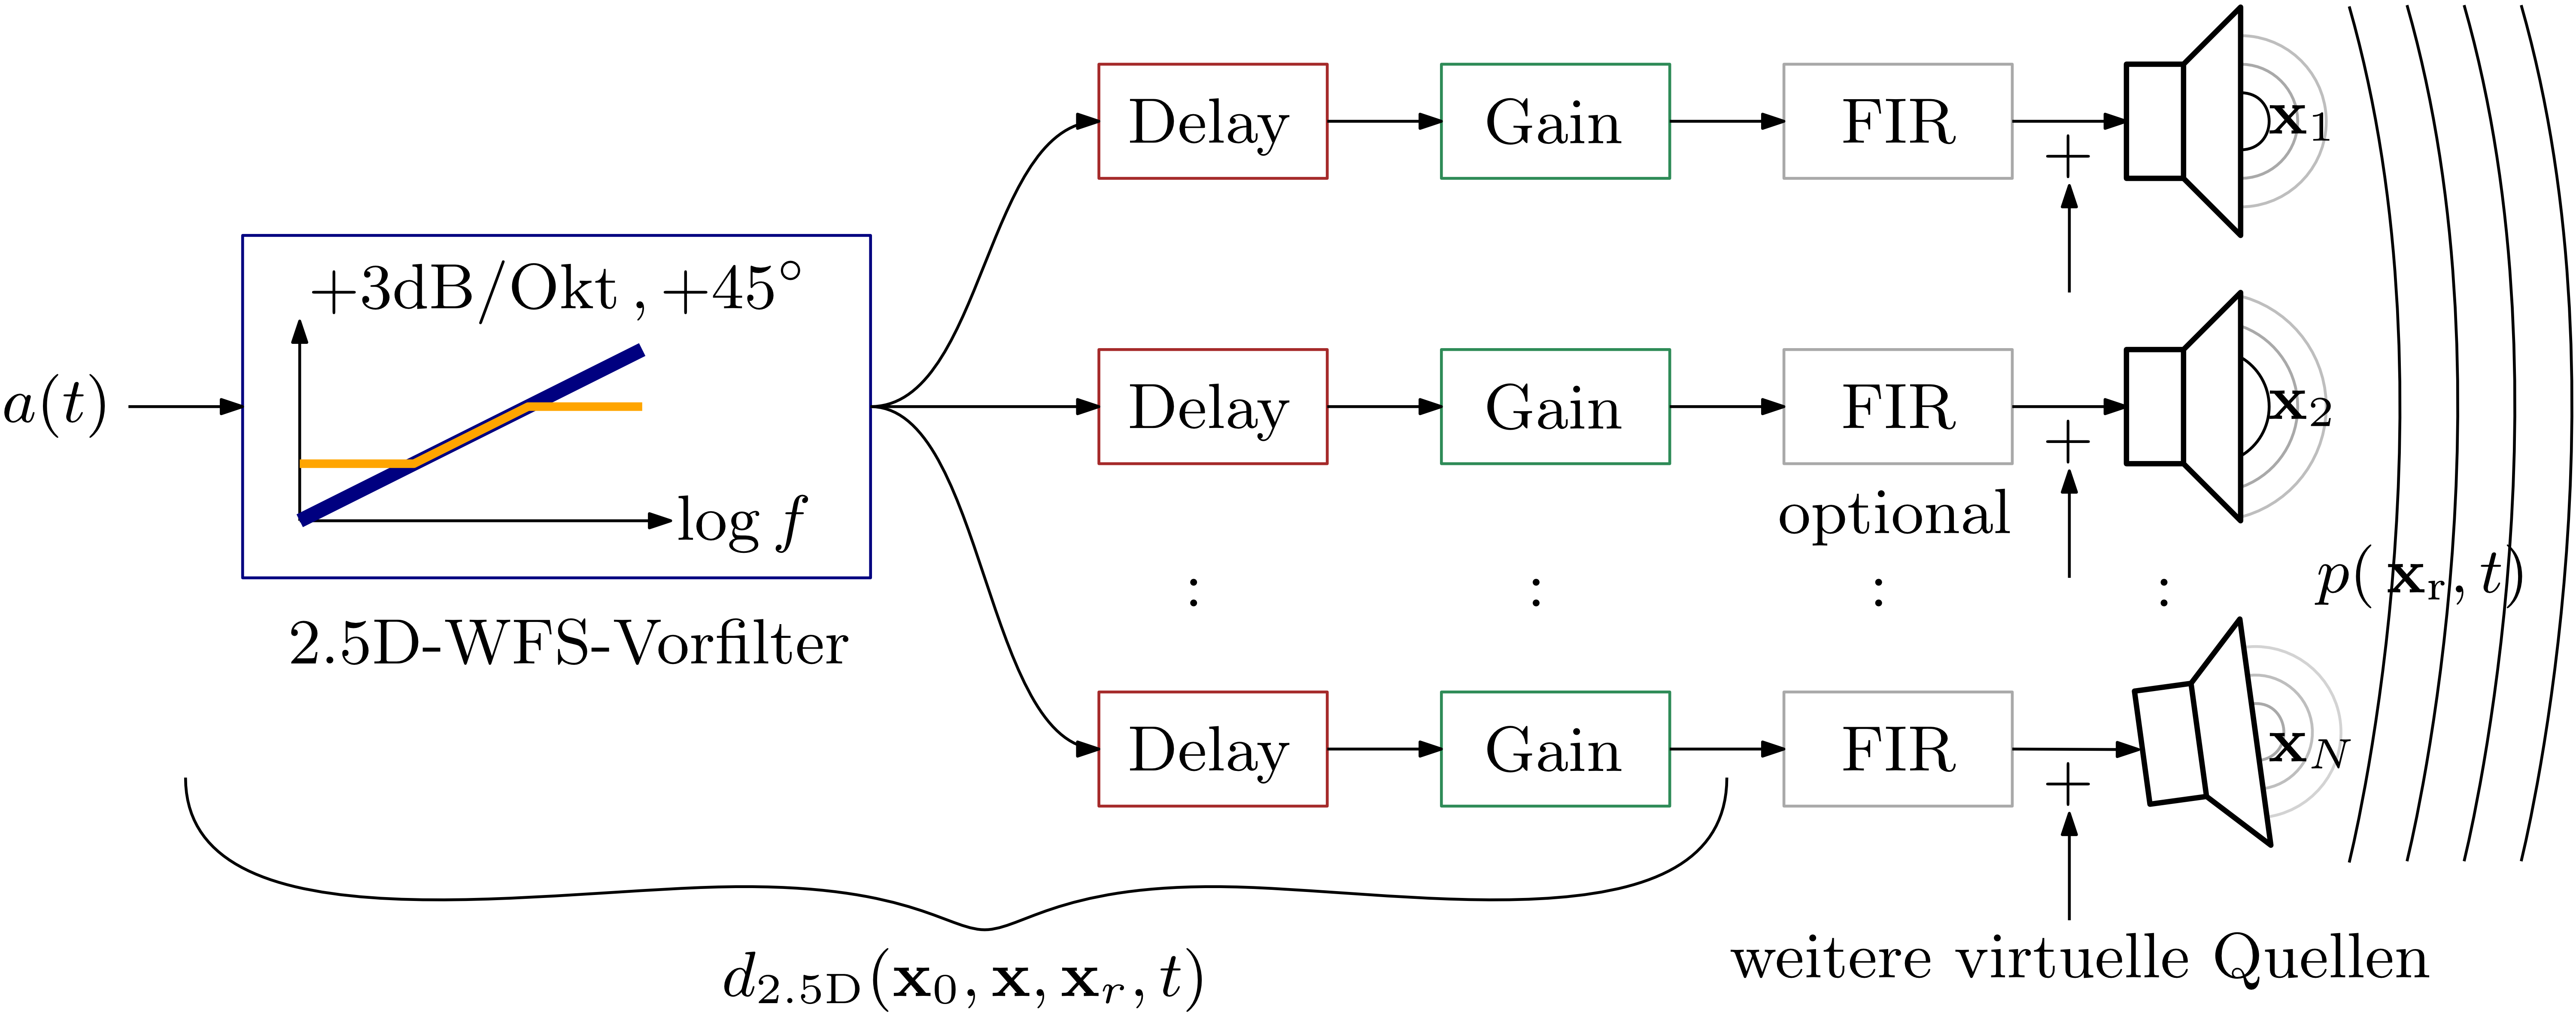
\includegraphics[width=145mm]{../graphics_DEU/WFS_Blockdiagramm.png}
\end{plotfigures}
\caption{Signalfluss von Audiosignal $a(t)$ zu Schalldruck $p(\xr, t)$
für die modellbasierte 2.5D-WFS.
Das Audio-Eingangssignal $a(t)$ wird zunächst mit dem sogenannten 2.5D-WFS-Vorfilter
\index{WFS-Vorfilter} gefiltert.
Danach folgen lautsprecherindividuelles Delay und Gain $\gain_\text{2.5D}$, welche sich aus der
Parametrik der virtuellen Quelle und Array-Geometrie ergeben,
siehe Treiberfunktion im Zeitbereich
in \Glg\eqref{eq:h25d_time}.
Die akustische Superposition von komplex gewichteten, akustischen Übertragungsfunktionen
$G(r_{\xs\text{-}\xr})$ führt zum Schalldruck $p(\xr, t)$.
Optionale Schallfeldoptimierung erfolgt typisch mit
lautsprecherindividuellen FIR-Filtern.
%
Die Superposition von Ansteuerungssignalen erlaubt die Synthese mehrerer virtueller
Quellen gleichzeitig.
%
\cc
}
\label{fig:WFS_Blockdiagramm}
\end{figure*}


Die Lösungen in \Glg\eqref{eq:Driving3D}, \eqref{eq:Driving25D}
für die Syntheseintegrale
\eqref{eq:MonopolIntegral_3D}, \eqref{eq:MonopolIntegral_25D}
sind nur dann eine valide Näherung, wenn -- neben Einhaltung
der Fernfeld-/Hochfrequenznäherung --
sowohl die Wellenlänge als auch die Wellenfrontkrümmung in Nähe der Hülle
deutlich kleiner als die räumliche Ausdehnung der aktiven Hüllfläche bzw. -kontur
(sogenannte Apertur\index{Apertur}) sind;
dies folgt aus der Theorie der Kirchhoff- bzw.
Fresnel-Kirchhoff-Beugung, für die WFS detailliert diskutiert in
\cite{Schultz2016_diss, Firtha2019_diss}.



\subsection{WFS-Ansteuerung im Zeitbereich}
\label{sec:WFS_Ansteuerung_im_Zeitbereich}
%
WFS-Signalverarbeitung im Zeitbereich erfordert pro Lautsprecher
einen individuellen Gain- und Delaywert, sowie ein spezielles Hochpassfilter,
vgl.~\Abb\ref{fig:WFS_Blockdiagramm} für die 2.5D-WFS.
%
Dies sind vergleichsweise einfache Operationen in der Signalverarbeitung.
%
Wegen Präzision und Flexibilität sollte die Umsetzung mit Digitaltechnik
erfolgen.
%
Das WFS-Ansteuerungsfilter im Zeitbereich, also die
Filter-Impulsantwort für den Monopol an der
Position $\xs$, wird für 3D-Synthese mit
\begin{align}
d_\text{3D}(\xp,\xs, t) =
\underbrace{\gain_\text{3D}(\xp,\xs)}_{\text{Gain}} \cdot
\underbrace{\delta(t-\frac{r_{\xs\text{-}\xp}}{c})}_{\text{Delay}} \,\ast_t\,
\underbrace{h_\text{3D,Pre}(t)}_{\text{Filter}}
\end{align}
und für 2.5D-Synthese mit
\begin{align}
d_\text{2.5D}(\xp,\xs,\xr, t) =
&\gain_\text{2.5D}(\xp,\xs,\xr) \times\nonumber\\
&\delta(t-\frac{r_{\xs\text{-}\xp}}{c}) \,\ast_t\,
h_\text{2.5D,Pre}(t)
\label{eq:h25d_time}
\end{align}
beschrieben.
%
Die Faltungsoperation $\ast_t$ bezüglich der Zeit $t$ ist die
korrespondierende Operation zur Multiplikation von $\omega$-abhängigen
Frequenzgängen.



Die $\im\frac{\omega}{c}$-unabhängigen Terme in den Filter-Frequenzgängen
in den \Glgn\eqref{eq:Driving3D}, \eqref{eq:Driving25D}
%
\begin{align}
&\gain_\text{3D}(\xp,\xs) = 2 \, \mathrm{max}\{-\nxT \, \bm{\theta}_{\xs\text{-}\xp}, 0\} \, \frac{1}{4\pi \, r_{\xs\text{-}\xp}}\\
%
&\gain_\text{2.5D}(\xp,\xs,\xr) =
\sqrt{2\pi}
\sqrt{\frac{r_{\xs\text{-}\xr} \cdot r_{\xs\text{-}\xp}}{r_{\xs\text{-}\xr} + r_{\xs\text{-}\xp}}}
\cdot \gain_\text{3D}(\xp,\xs)\nonumber\\
&={\frac{1}{\sqrt{2\pi}}}
\sqrt{\frac{r_{\xs\text{-}\xr}}{r_{\xs\text{-}\xr} + r_{\xs\text{-}\xp}}} \frac{1}{\sqrt{r_{\xs\text{-}\xp}}}
\,\mathrm{max}\{-\nxT \, \bm{\theta}_{\xs\text{-}\xp}, 0\}
\end{align}
%
verhalten sich bezüglich der Fourier-Transformation wie konstante Faktoren, treten
daher im Frequenz- und Zeitbereich gleich auf.
%
Diese stellen die lautsprecherindividuellen Gewichte (\textit{gain}) für den
3D-~bzw.~2.5D-Fall dar.
%
Im 3D-Fall ist das Gewicht pro Lautsprecher nur von der Position $\xp$  der
virtuellen Punktquelle und natürlich von der Lautsprecherposition $\xs$ abhängig.
%
Im 2.5D-Fall ergibt sich eine zusätzliche Abhängigkeit zu genau dem Empfängerpunkt
$\xr(\xs)$, für den eine amplitudenkorrekte Synthese realisiert werden soll,
vgl.~\Abb\ref{fig:25DWFS_Schema}.



In den Filter-Frequenzgängen in den \Glgn\eqref{eq:Driving3D}, \eqref{eq:Driving25D}
resultiert für den in $G(r_{\xs\text{-}\xp},\omega)$ (vgl.~\Glg\eqref{eq:G03D})
auftretenden komplexen Zeiger
$\e^{-\im\wc r_{\xs\text{-}\xp}}$
die zeitliche Korrespondenz
\begin{align}
\e^{-\im\wc r_{\xs\text{-}\xp}}
\quad\Laplace\quad
\delta\left(t-\frac{r_{\xs\text{-}\xp}}{c}\right)
\end{align}
aus inverser Fourier-Transformation (angedeutet mit dem Operator $\,\Laplace\,$).
%
Dies liefert den um
$\tau_\text{Delay}=\frac{r_{\xs\text{-}\xp}}{c}$
verzögerten Dirac-Impuls
$\delta(t)$.
%
Es handelt sich somit um eine Verzögerung (\textit{delay}) und
bildet die von der Schallgeschwindigkeit $c$ abhängige Laufzeit des Schalls
von der virtuellen Quelle bei $\xp$ zum jeweilig betrachteten Lautsprecher bei
$\xs$ ab.
%
Aus den \Glgn\eqref{eq:Driving3D}, \eqref{eq:Driving25D} sind nun noch die
$\im\frac{\omega}{c}$-abhängigen Terme
%
\begin{align}
&H_\text{3D,Pre}(\omega) = \im\frac{\omega}{c} \quad\Laplace\quad h_\text{3D,Pre}(t)
\label{eq:Prefilter3D}\\
%
&H_\text{2.5D,Pre}(\omega) = \frac{\im\frac{\omega}{c}}{\sqrt{\im\frac{\omega}{c}}} = \sqrt{\im\frac{\omega}{c}} \quad\Laplace\quad h_\text{2.5D,Pre}(t)
\label{eq:Prefilter25D}
\end{align}
%
für den 3D-~bzw.~2.5D-Fall zu diskutieren.
%
Diese Frequenzgänge beschreiben Hochpässe, die den inhärenten
spektralen Tiefpasscharakter der Hüllfläche bzw. -kontur kompensieren.
%
Im 3D-Fall hat der kompensierende Hochpass eine Flanke von $+6$\,dB/Oktave mit
$+90^\circ$ konstantem Phasenverlauf, im 2.5D-Fall hat das kompensierende Filter
eine Flanke von $+3$\,dB/Oktave mit $+45^\circ$ konstanter Phase.
%
Da die Hochpassfilter in den \Glgn\eqref{eq:Prefilter3D}, \eqref{eq:Prefilter25D}
unabhängig von der virtuellen Quelle sind, erscheint es ganz vernünftig,
das Audio-Eingangssignal $a(t)$ damit vorzufiltern -- dies führt auf den
oft benutzten, englischen Begriff
\textit{WFS pre-filtering}\index{WFS pre-filtering} -- und
erst danach die lautsprecherindividuellen Verzögerungen und Gewichte
auf das vorgefilterte Signal anzuwenden.
%
\Abb\ref{fig:WFS_Blockdiagramm} verdeutlicht die beschriebenen
Verarbeitungsschritte in einem Signalflussgraphen.



Das Schallfeld -- genauer die räumliche Ausbreitung der Wellenfront über die
Zeit -- einer virtuellen Quelle mit der Ansteuerung des Audiosignals
$a(t) \,\,\laplace\,\, A(\omega)$
wird mittels der WFS also synthetisiert, indem die lautsprecherindividuelle
Faltung $a(t) \ast_t d(t)$ (elektrische Ansteuerung) realisiert wird und
sich die ausbreitenden Schallfelder der Lautsprecher zur gewünschten Wellenfront
überlagern (akustisches Resultat).
%
In der Praxis wird die Faltung $a(t) \ast_t d(t)$, wie oben diskutiert,
oft aufgeteilt in Hochpassfilter, Delay und Gain.



\section{Simulationen für die WFS einer virtuellen Punktquelle}
\label{sec:WFS_PointSource_Simulationen}
%
In diesem Abschnitt illustrieren Ergebnisse von numerischen Simulationen die
Funktionsweise und die wichtigsten Eigenschaften von 2.5D-WFS,
vgl. \cite{Berkhout1993_JASA,Boone1995_JAES,Start1997_diss,Spors2010a}.
%
Die Simulationen beruhen auf dem obigen Formelapparat für 2.5D-WFS
und können z.B. mit der Sound Field Synthesis
Toolbox \cite{Winter2019dagaposter}\footnote{\url{https://github.com/sfstoolbox}}
und der Referenzimplementierung zu diesem
Kapitel\footnote{\url{https://github.com/spatialaudio/wfs_chapter_hda}}
nachvollzogen und durchgeführt werden.
%
Für alle folgenden Simulationen ist die Schallgeschwindigkeit $c=343$\,m/s.
%
Zunächst werden monofrequente Schallfelder in den
%\Abb\ref{fig:wfs25d_lineSSD},~\ref{fig:wfs25d_circSSD},~\ref{fig:wfs25d_lineSSD_truncation},~\ref{fig:wfs25d_lineSSD_aliasing},~\ref{fig:wfs25d_lineSSD_polar_plot_overlay},~\ref{fig:wfs25d_circSSD_aliasing},
\Abb\ref{fig:wfs25d_lineSSD} bis \ref{fig:wfs25d_circSSD_aliasing},
und anschließend
%in fig:td_0m_noaliasing \Abb\ref{fig:td_-1m},~\ref{fig:td_0m},~\ref{fig:td_1m}
impulsartige Schallfelder im Zeit- und Frequenzbereich
in den \Abb\ref{fig:td_0m_noaliasing} bis \ref{fig:td_1m}
diskutiert.



\subsection{Nah-/Fernfeld vs. Wellenfront-/Abstrahlsynthese}
%
Vorangestellt sei noch, dass sich die folgende Diskussion des Konzepts der Fraunhofer-
bzw. Fresnel-Region \cite[Kap.~26]{Skudrzyk1971} bedient: Interferenzeffekte
sind an verschiedenen Empfängerpunkten näherungsweise analytisch zugänglich und
damit aus Formeln heraus interpretierbar.
%
Das Konzept wird hier stark vereinfacht benutzt und die Fraunhofer-Region mit dem
Fernfeld\index{Fernfeld} bzw. die Fresnel-Region mit dem
Nahfeld\index{Nahfeld} endlicher Lautsprecherarrays gleichgesetzt.
%
Für eine endlich große Quelle mit größter Abmessung $l$ (d.h. die aktive Apertur)
befindet sich ein Messpunkt mit Quellenabstand $R$ im Fernfeld, wenn die
drei Kriterien
a) $R \gg l$,
b) $\frac{R}{l} \gg \frac{l}{\lambda}$ und
c) $R \gg \lambda$ (ähnlich der oben gemachten Fernfeld-/Hochfrequenznäherung
$\frac{\omega}{c} R \gg 1$) erfüllt werden, vgl. \cite[Kap.~3.5.4]{Moeser2015_book}.
%
Würde der Schalldruck um das mit den Treiberfunktionen angesteuerte,
endliche Lautsprecherarray auf einer Kugeloberfläche erfasst, würde sich ab einer
bestimmten Entfernung -- der aus den Bedingungen a) bis c) resultierenden,
frequenzabhängigen Nah-/Fernfeldgrenze -- eine
frequenzabhängige
Fernfeldrichtcharakteristik\index{Fernfeldrichtcharakteristik} ausprägen, welche in
noch weiterer Entfernung vom Array
$6$\,dB-Pegelverlust pro Entfernungsverdopplung verzeichnet.



Bei Schallfeldsynthese wird gezielt Interferenz erzeugt, so dass sich im Nahfeld des
Lautsprecherarrays die gewünschte Wellenfrontkrümmung mit charakteristischer
Amplitudenabnahme ergibt.
%
Hingegen wird bei Abstrahlsynthese (\textit{beam forming}) gezielt mit
Interferenz gearbeitet, um eine gewünschte Fernfeldrichtcharakteristik zu
realisieren.
%
Die Wellenfrontkrümmung im Fernfeld einer Quelle ist wegen des $6$\,dB-Pegelverlustes
immer punktquellenartig,
%
auch wenn in einem räumlich begrenzten Bereich in sehr weitem Abstand zur Quelle
diese Krümmung verschwindend klein erscheinen kann.
%
Dieser Effekt wird genau bei der Modellierung der virtuellen ebenen Welle mittels
einer sehr weit entfernten virtuellen Punktquelle ausgenutzt.







\subsection{Monofrequentes Schallfeld}
%
\Abb\ref{fig:wfs25d_lineSSD} zeigt die 2.5D-WFS einer virtuellen Punktquelle
mit sekundären Monopolquellen infinitesimalen Abstands entlang einer unendlich
langen Linie auf der $y$-Achse.
%
% please DO NOT rescale the figure and keep it single column
\begin{figure}[t]
\centering
\begin{plotfigures}
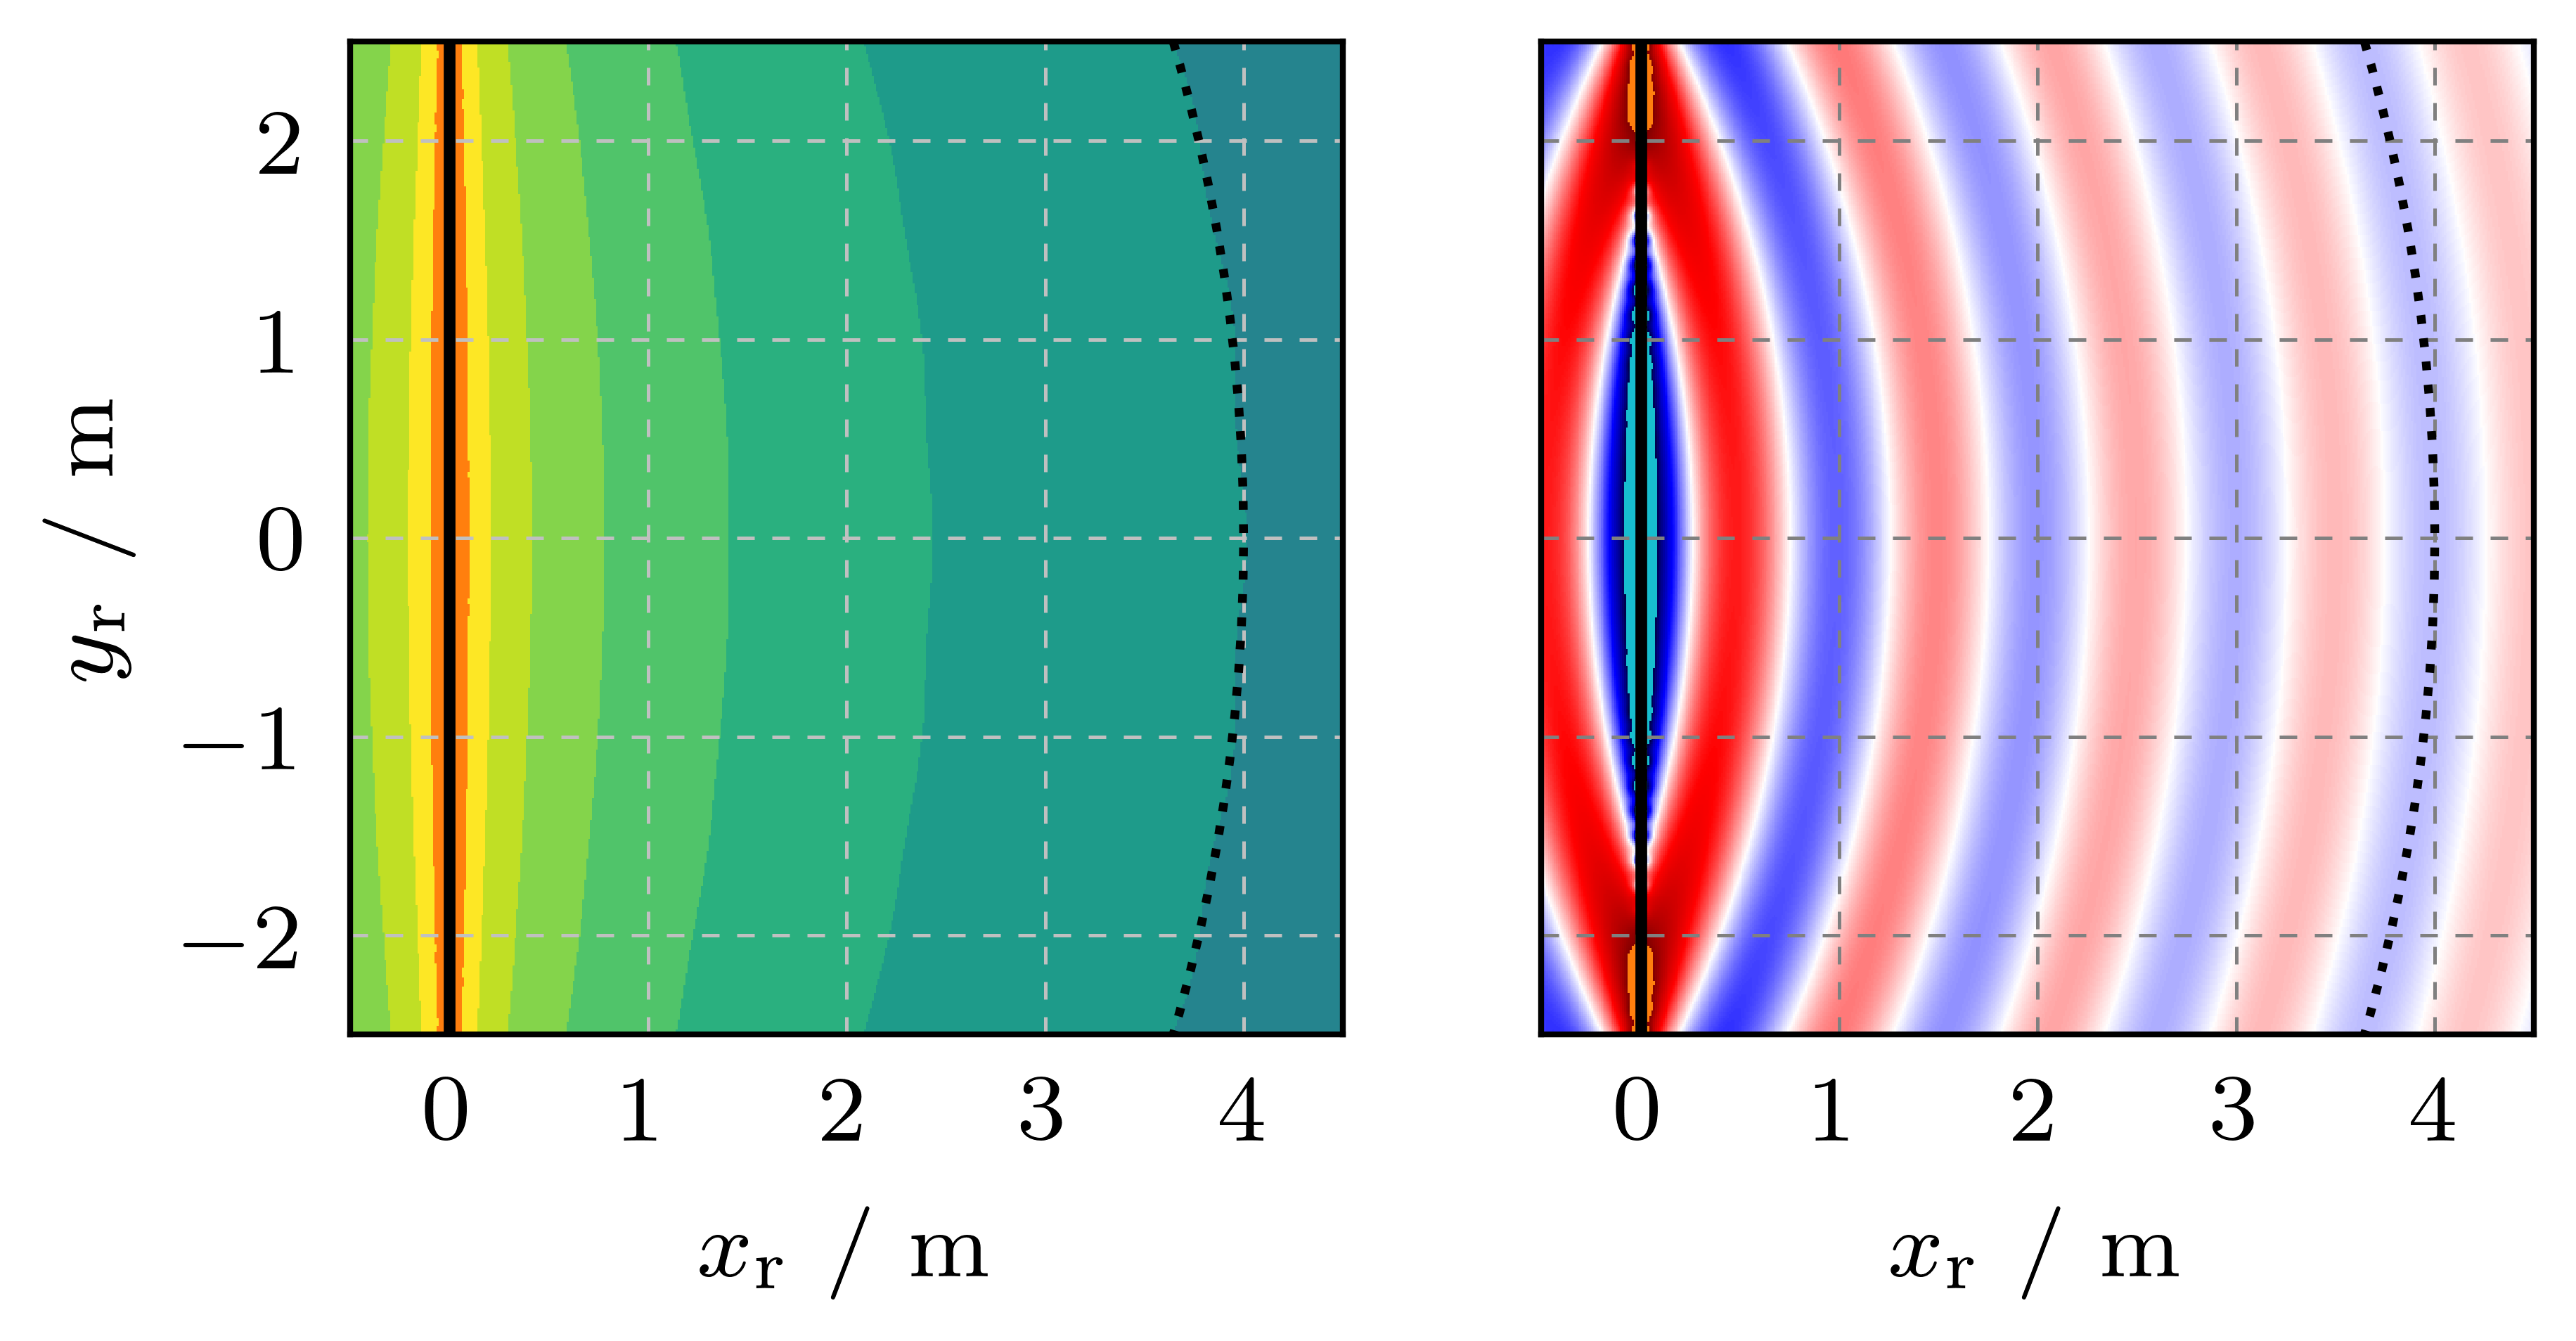
\includegraphics[width=85mm]{../python/wfs25d_lineSSD.png}
\end{plotfigures}
\caption{2.5D-WFS einer virtuellen Punktquelle bei $\xp = (-5,0,0)^\mathrm{T}$\,m
mit einem unendlichen Monopol-Array auf der $y$-Achse (schwarz) für
die Wellenlänge $\lambda=1$\,m.
%
Entlang der Referenzkurve -- der gestrichelte, schwarze Kreisbogen -- erfolgt eine
Amplitudenkorrektur auf Schalldruckamplitude Eins (rechts) bzw. $0$\,dB-Schalldruckpegel (links).
%
Schallfeld mit deutlich erkennbarer Kugel-Wellenfrontkrümmung und gezeigtem
Zeitbezug für einen Schalldruckwert~$-1$ entlang der Referenzkurve.
%
Farbskalierung wie in \Abb\ref{fig:plot_colorbar}.
\cc
}
\label{fig:wfs25d_lineSSD}
\end{figure}
%
Amplitudenkorrekte Synthese ergibt sich entlang des eingezeichneten Kreisbogens,
der den Punkt $\xr = (4,0,0)^\mathrm{T}$\,m schneidet.
%
Die Wellenfrontkrümmung\index{Wellenfrontkrümmung} einer Punktquelle ist ersichtlich.
%
Da für das unendlich lange Array kein Nah-/Fernfeldübergang existiert,
bleibt die gewünschte Wellenfrontkrümmung der virtuellen Quelle
über alle Entfernungen erhalten.
%
Die für 2.5D-WFS charakteristische Schalldruckamplitudenabnahme
kann mit \Glg\eqref{eq:pStat25D} quantitativ für ein Punktpaar
stationärer Phase beschrieben werden.
%
Wenn Schalldrücke und Pegel jenseits der pegelrichtigen Referenzkurve von
Interesse sind, muss diese nichtlineare Funktion bezüglich $\xs$, $\xr$ und
der Primärquellenposition
$\xp$ (welche die Wellenfrontkrümmung beeinflusst) analysiert
werden, vgl. \cite{Sonke2000_diss,Wittek2007_diss, Spors2010a}.
%
Dies ist in der 2.5D-WFS-Praxis (bzw. allgemeingültig für alle
2.5D-Schallfeldsyntheseverfahren) vor allem dann relevant, wenn mehrere virtuelle
Quellen gleichzeitig und näherungsweise pegelrichtig für einen größeren
Zuhörerbereich synthetisiert werden sollen.



In \Abb\ref{fig:wfs25d_circSSD} wird ein kreisförmiges,
kontinuierliches Monopol-Array benutzt.
%
% please DO NOT rescale the figure and keep it single column
\begin{figure}[t]
\centering
\begin{plotfigures}
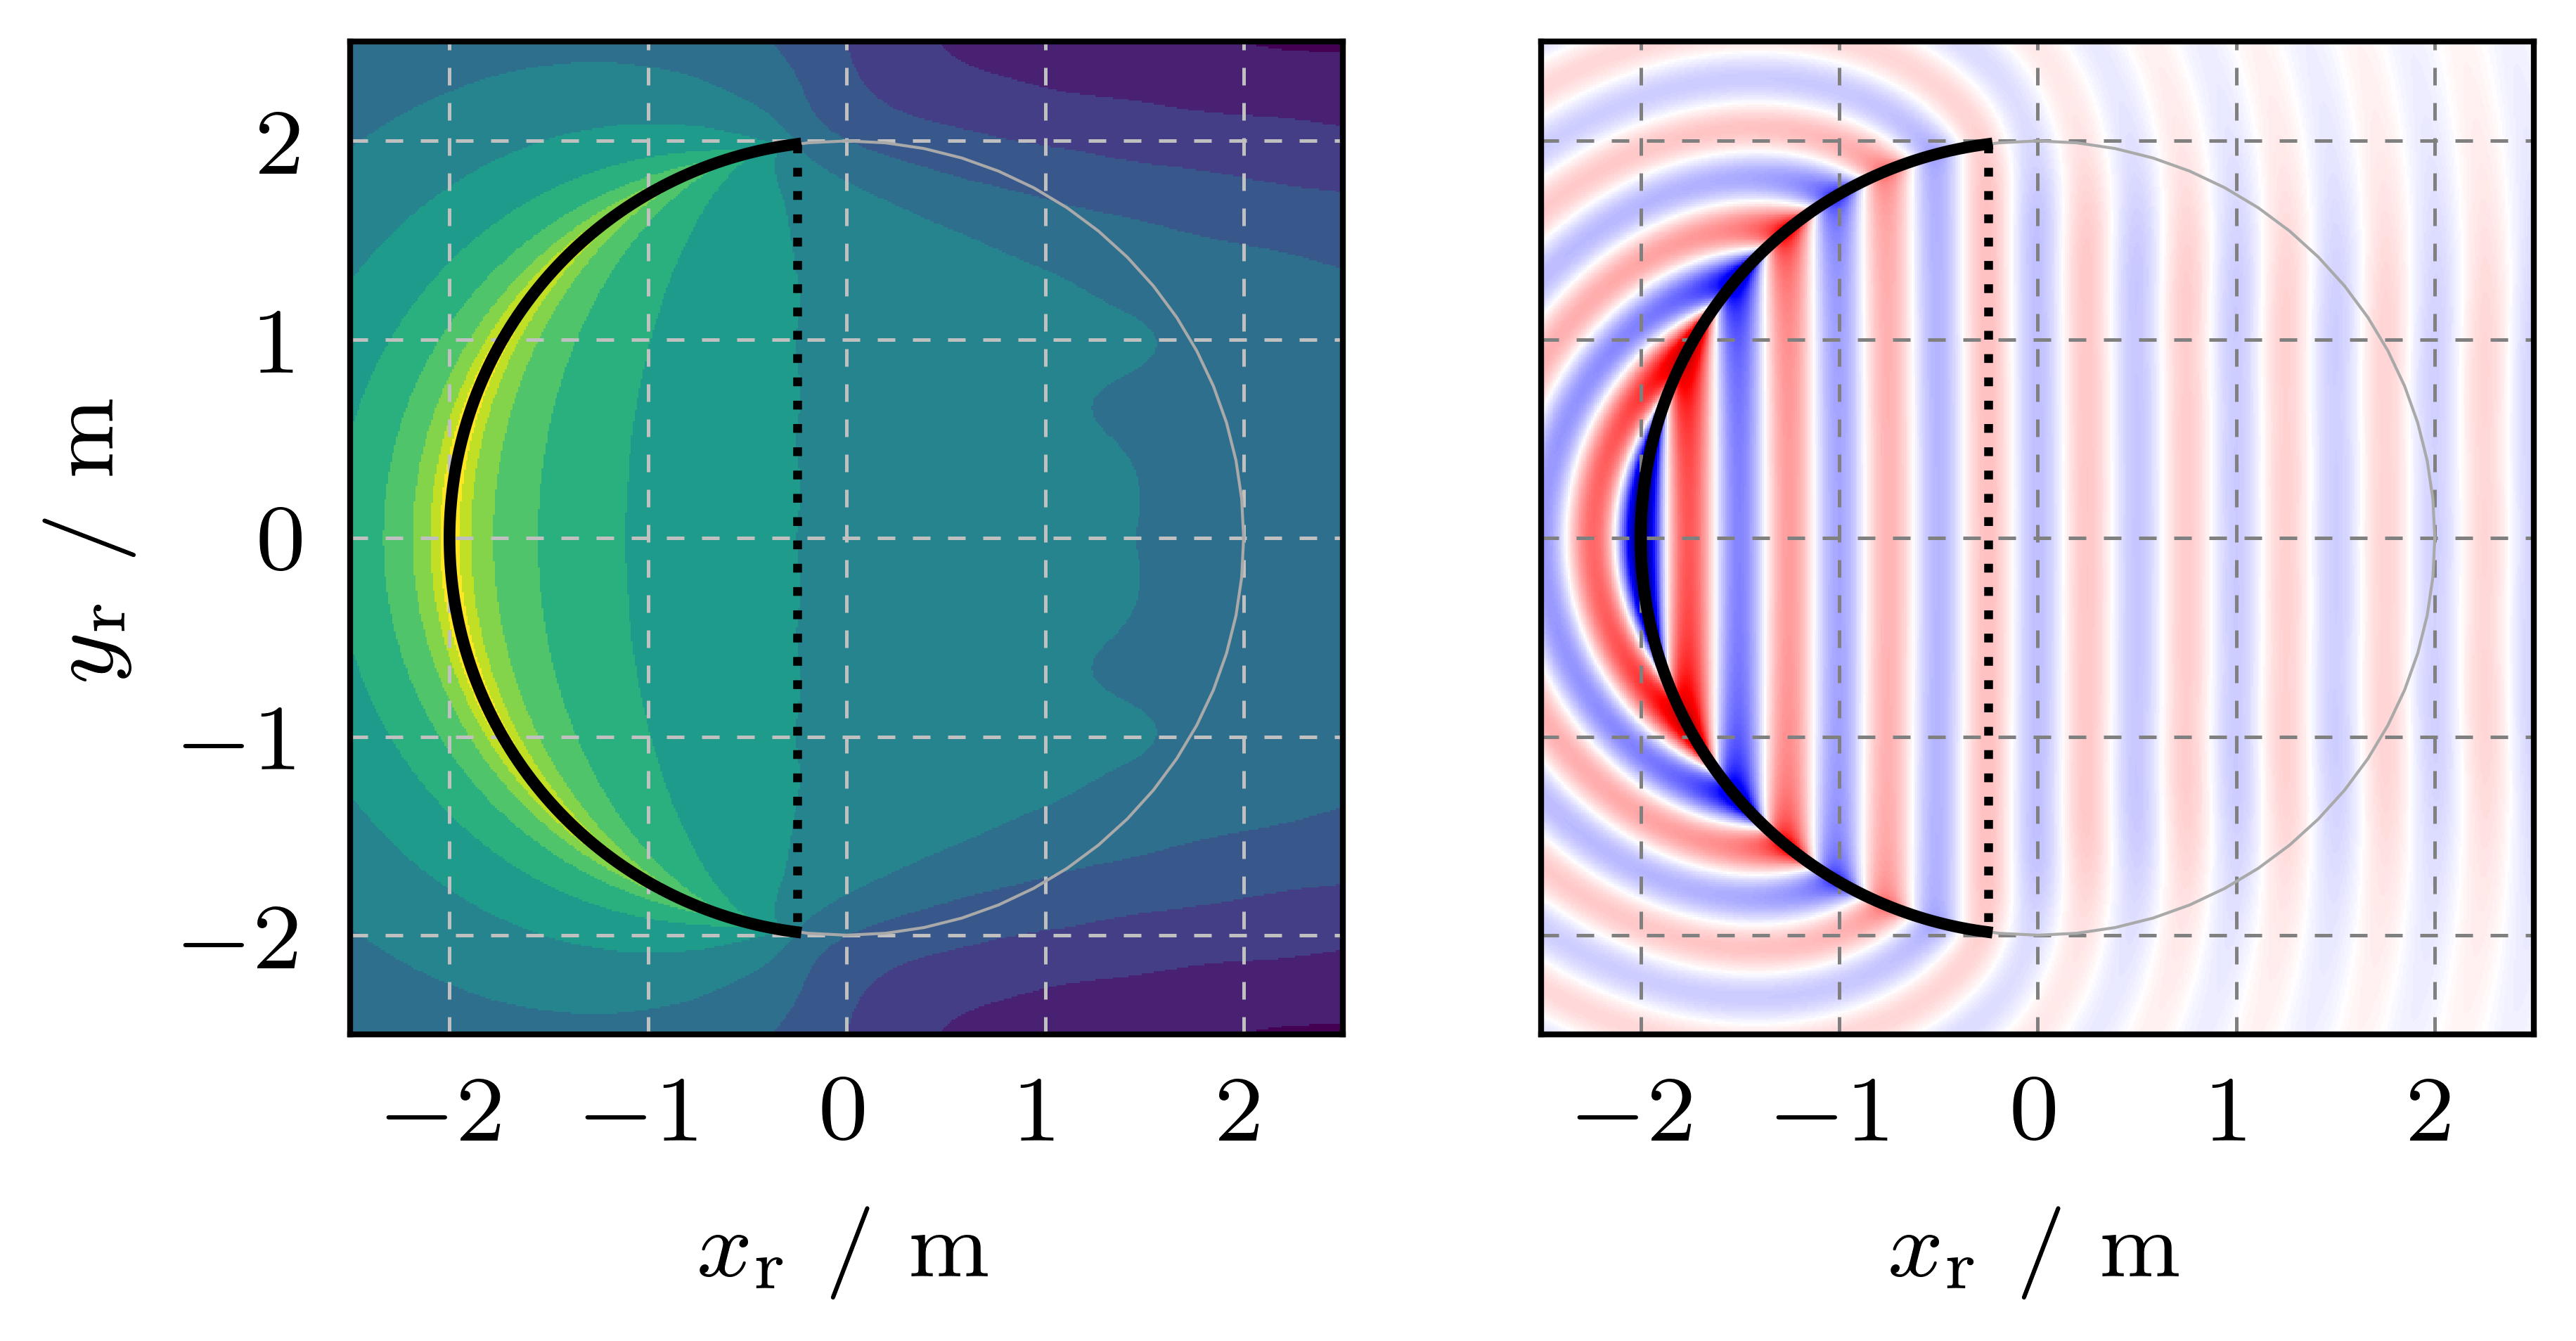
\includegraphics[width=85mm]{../python/wfs25d_circSSD.png}
\end{plotfigures}
\caption{2.5D-WFS einer virtuellen Punktquelle bei $\xp = (-100,0,0)^\mathrm{T}$\,m
mit einem 2\,m-Radius-Kreisarray (aktiv beitragende Monopole in schwarz, vgl.~\eqref{eq:SecSrcSel})
für die Wellenlänge $\lambda=\frac{1}{2}$\,m.
%
Entlang der Referenzkurve -- hier die gestrichelte schwarze Linie bei
$x=-\frac{1}{4}$\,m -- erfolgt
eine Amplitudenkorrektur auf Schalldruckamplitude Eins bzw. $0$\,dB-Schalldruckpegel.
%
%
Schallfeld, mit im Zuhörerbereich verschwindender Wellenfrontkrümmung, visualisiert
für einen Zeitpunkt bei dem Schalldruckwert~$+1$ entlang der Referenzlinie vorliegt.
%
\cc
}
\label{fig:wfs25d_circSSD}
\end{figure}
%
2.5D-WFS einer ebenen Wellenfront -- also eine Welle
mit verschwindender Wellenfrontkrümmung innerhalb der Zuhörerfläche -- wurde
mit einer sehr weit entfernten virtuellen Punktquelle angenähert.
%
Amplitudenkorrekte Synthese erfolgt für \Abb\ref{fig:wfs25d_circSSD}
auf der Linie bei $x=-\frac{1}{4}$\,m.
%
Für alle anderen Empfängerpunkte gilt wieder die in 2.5D-WFS
charakteristische Schalldruckamplitudenabnahme im Nahfeld des Arrays.
%
Im frequenzabhängigen Fernfeld des Arrays geht die ebene Wellenfrontkrümmung
(virtuelle Quelle) in die einer Punktquelle (Lautsprecherarray) über,
einhergehend mit $6$\,dB-Pegelverlust pro Entfernungsverdopplung.



In \Abb\ref{fig:wfs25d_lineSSD_truncation} ist die 2.5D-WFS einer ebenen
Wellenfront mit einem linearen, auf der $y$-Achse liegenden, endlichen
Monopol-Array visualisiert.
%
% please DO NOT rescale the figure and keep it single column
\begin{figure}[t]
\centering
\begin{plotfigures}
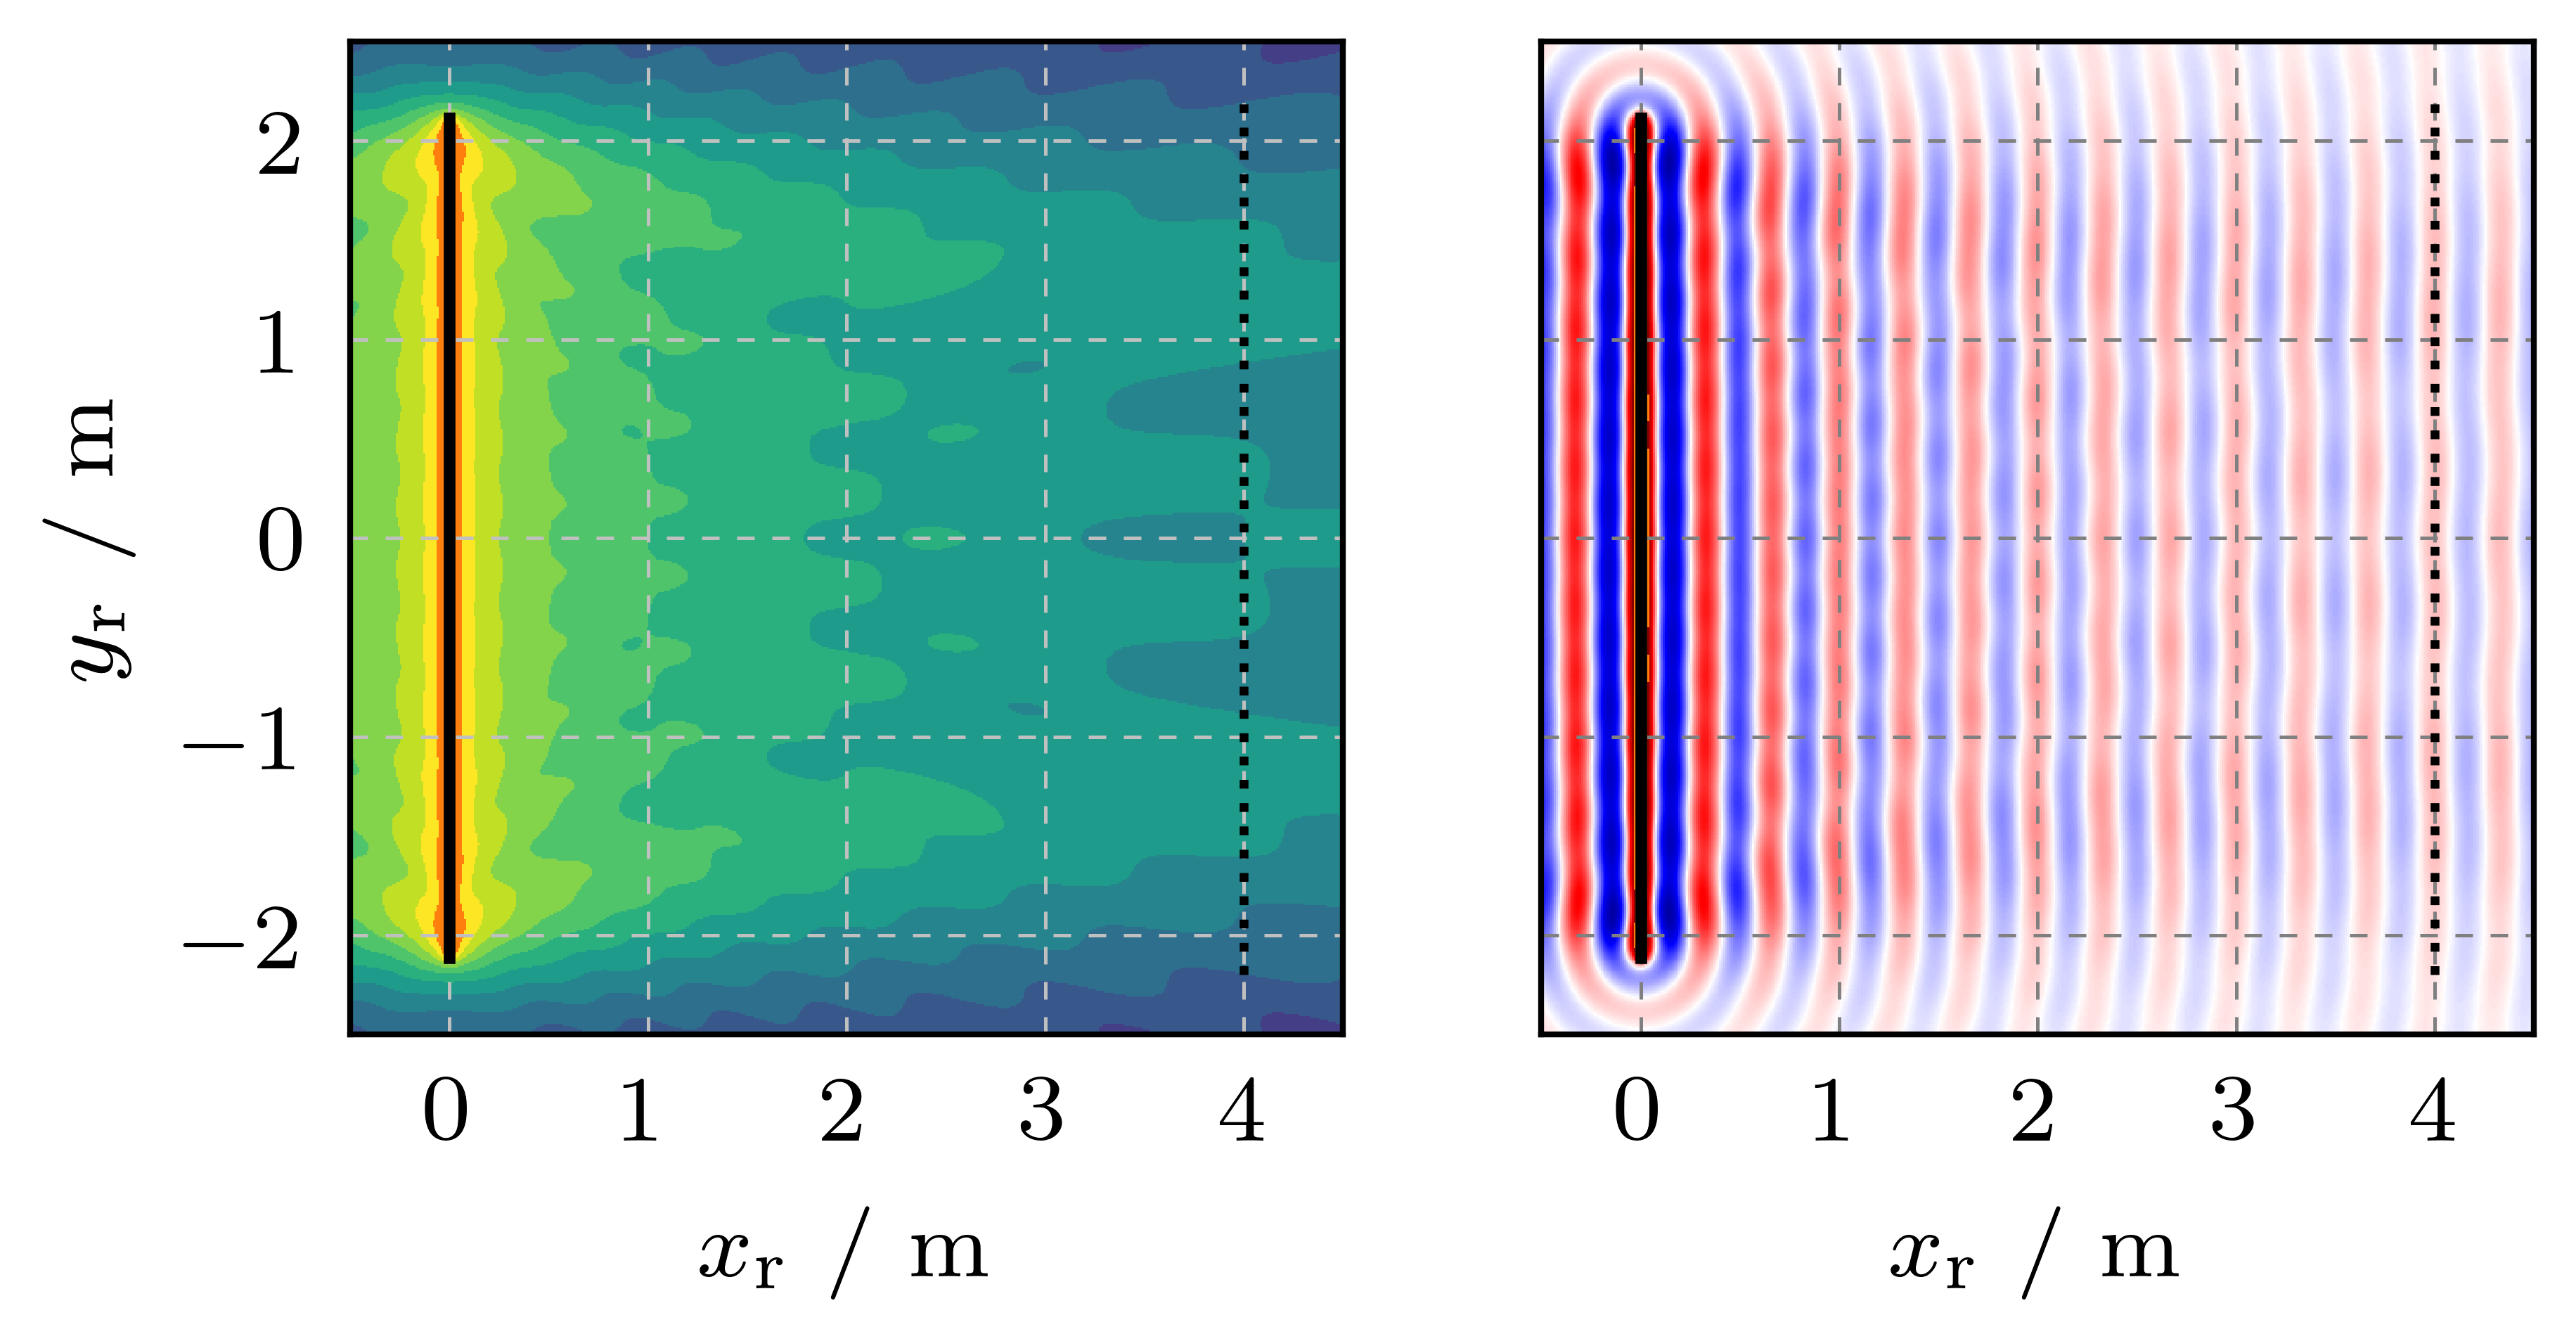
\includegraphics[width=85mm]{../python/wfs25d_lineSSD_truncation.png}
\end{plotfigures}
\caption{2.5D-WFS einer virtuellen Punktquelle bei
$\xp = (-100,0,0)^\mathrm{T}$\,m mit endlichem, kontinuierlichen Monopol-Array
entlang der $y$-Achse für die Wellenlänge $\lambda=\frac{1}{3}$\,m.
%
Amplitudenkorrektur auf $0$\,dB-Pegel entlang der schwarz-gestrichelten
Referenzlinie bei $x=4$\,m.
%
%Die 21 weißen Punkte auf dieser bilden mit den 21 Monopolen jeweils ein
%Punktpaar mit stationärer Phasenbedingung.
%
Beugung an einem endlichem Array:
Wellen mit anderen Laufrichtungen beeinträchtigen die
gewünschte ebene Wellenfront im Nahfeld des Arrays. Im Fernfeld des Arrays
bildet sich die linke Richtcharakteristik in
\Abb\ref{fig:wfs25d_lineSSD_polar_plot_overlay} aus.
%
\cc
}
\label{fig:wfs25d_lineSSD_truncation}
\end{figure}
%
Die ebene Wellenfront weist wegen frequenzabhängiger Beugung Artefakte auf.
%
Diese lassen sich anschaulich mit der in
\Abb\ref{fig:wfs25d_lineSSD_polar_plot_overlay}~(links)
dargestellten Fernfeldrichtcharakteristik der gewählten Frequenz erklären.
%
Nebenkeulen korrespondieren mit Wellenfronten im Nahfeld, welche die im
Polardiagramm indizierten -- im Vergleich zur $0^\circ$-Hauptrichtung der ebenen
Wellenfront -- anderen Abstrahlrichtungen  aufweisen.
%
Die Wellenfronten interferieren und erzeugen so die Beugungsartefakte.
%
% please DO NOT rescale the figure and keep it single column
\begin{figure}[t]
\centering
\begin{plotfigures}
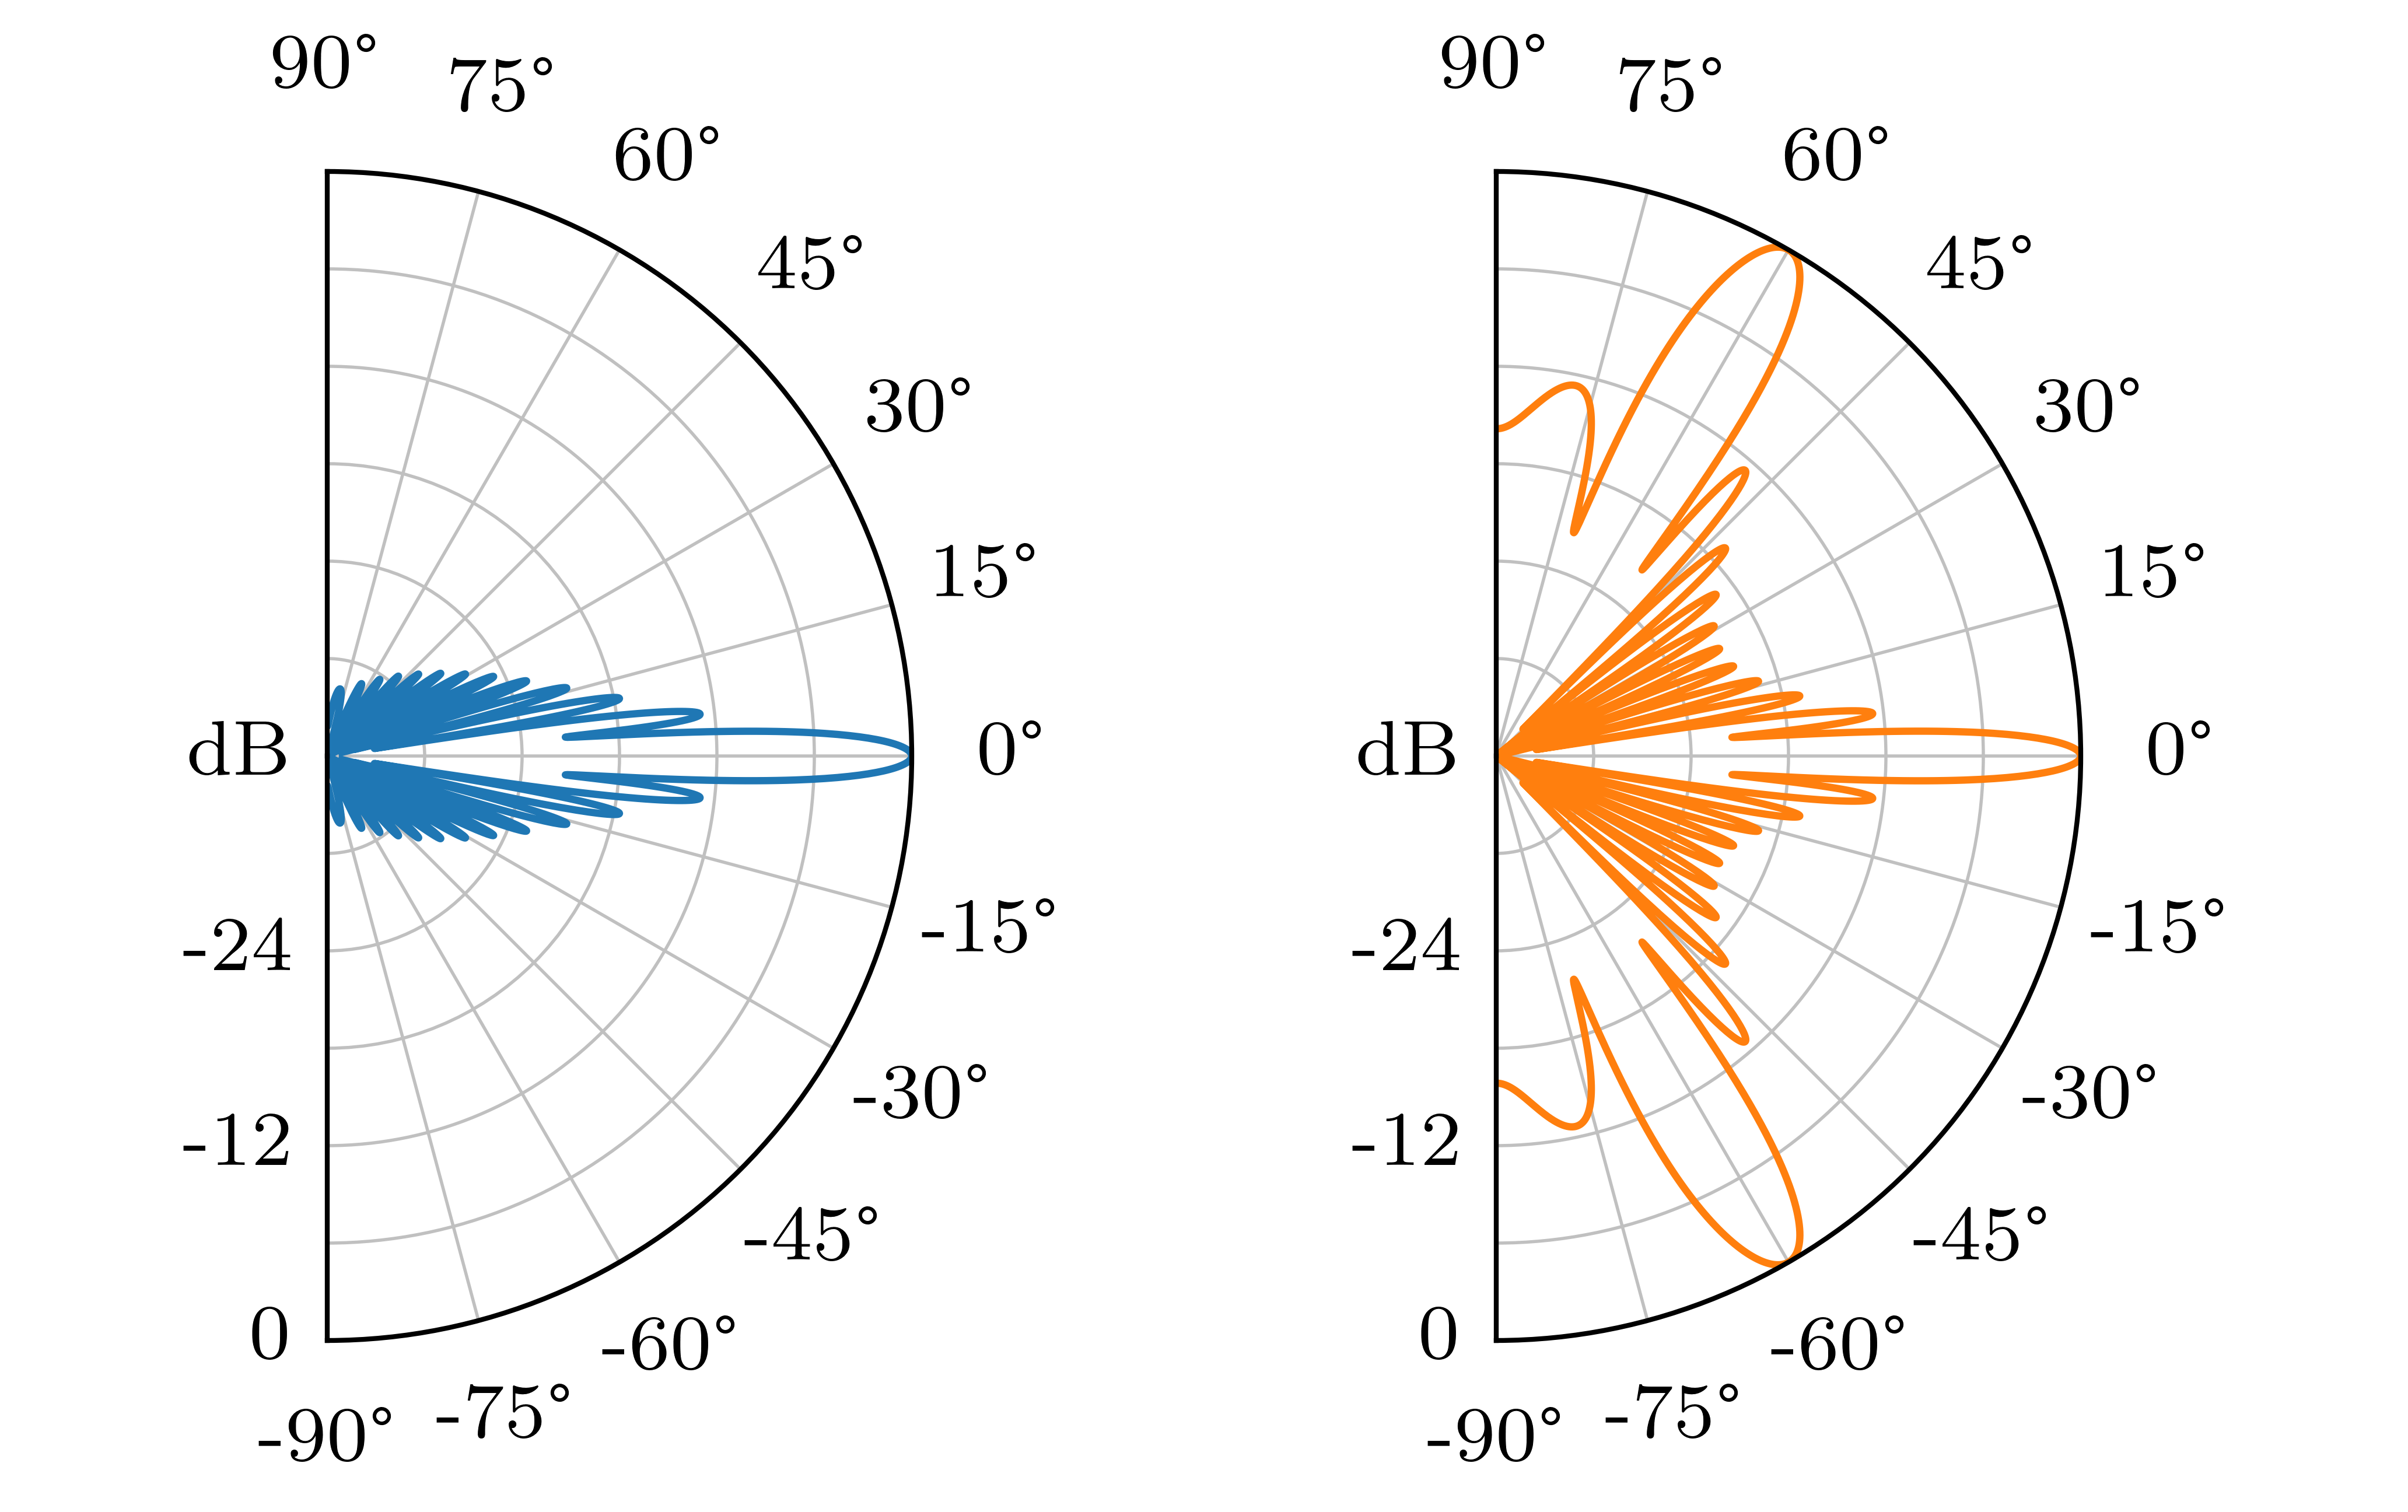
\includegraphics[width=85mm]{../python/wfs25d_lineSSD_polar_plot_overlay.png}
\end{plotfigures}
\caption{
Fernfeldrichtcharakteristiken für
Wellenlänge $\lambda=\frac{1}{3}$\,m, $\frac{2\pi}{\lambda} L \approx 79{,}807$
und gleicher virtueller Primärquelle, aber
verschiedene Sekundärquellenverteilungen.
Links, blau für \Abb\ref{fig:wfs25d_lineSSD_truncation} und
rechts, orange für \Abb\ref{fig:wfs25d_lineSSD_aliasing}.
%
Das Szenario aus \Abb\ref{fig:wfs25d_lineSSD_truncation} erzeugt im Fernfeld
eine $0^\circ$-Hauptkeule\index{Hauptkeule}
(\textit{main lobe}\index{main lobe})
und viele Nebenkeulen\index{Nebenkeule}
(\textit{side lobes}\index{side lobe}).
%
Das Szenario aus \Abb\ref{fig:wfs25d_lineSSD_aliasing} erzeugt im Fernfeld zusätzlich
zur $0^\circ$-Hauptkeule für die gewählte Wellenlänge zwei etwas breitere
Gitterkeulen\index{Gitterkeule} (\textit{grating lobes}\index{grating lobe})
bei exakt $\pm 60^\circ$ mit gleichem Pegel, sowie viele Nebenkeulen.
%
Gitterkeulen stehen in Verbindung zu räumlichem Aliasing, Nebenkeulen zu Beugung.
%
\cc
}
\label{fig:wfs25d_lineSSD_polar_plot_overlay}
\end{figure}
%
Die Pegel der Nebenkeulen und damit die Beugungsartefakte lassen sich durch
sogenanntes \textit{tapering} bzw. \textit{gain shading},
vgl. \cite{Vogel1993_diss,Start1997_diss}, verringern.
%
Dies geht jedoch immer zu Kosten einer breiteren Hauptkeule
im Fernfeld (vgl. kompromissbehaftetes Fensterdesign in der Signalverarbeitung,
\cite[Kap.~3.5]{Moeser2015_book}, \cite{Kammeyer2022_book}) und wirkt sich
daher im Nahfeld auch auf die gewünschte $0^\circ$-Wellenfront aus.



In \Abb\ref{fig:wfs25d_lineSSD_aliasing} ist die 2.5D-WFS einer ebenen Wellenfront
mit einem endlichen, linearen Monopol-Array entlang der $y$-Achse visualisiert.
%
Die Arraylänge $L \approx 4{,}234$\,m und die Wellenlänge $\lambda=\frac{1}{3}$\,m sind
gleich gewählt wie bei \Abb\ref{fig:wfs25d_lineSSD_truncation}.
%
Nun aber weisen die sekundären Monopole einen Abstand von
$\Delta_{\xs}\approx 0{,}3849$\,m auf; das Array ist räumlich diskretisiert.
%
Für dieses Szenario treten neben Beugungsartefakten zusätzlich
frequenzabhängige Artefakte auf, welche auf den endlichen Abstand der
Sekundärquellen zurückzuführen sind.
%
Diese Artefakte sind bekannt als räumliches Aliasing und beeinträchtigen die
gewünschte Wellenfront deutlich ausgeprägter als Beugung.
%
% please DO NOT rescale the figure and keep it single column
\begin{figure}[t]
\centering
\begin{plotfigures}
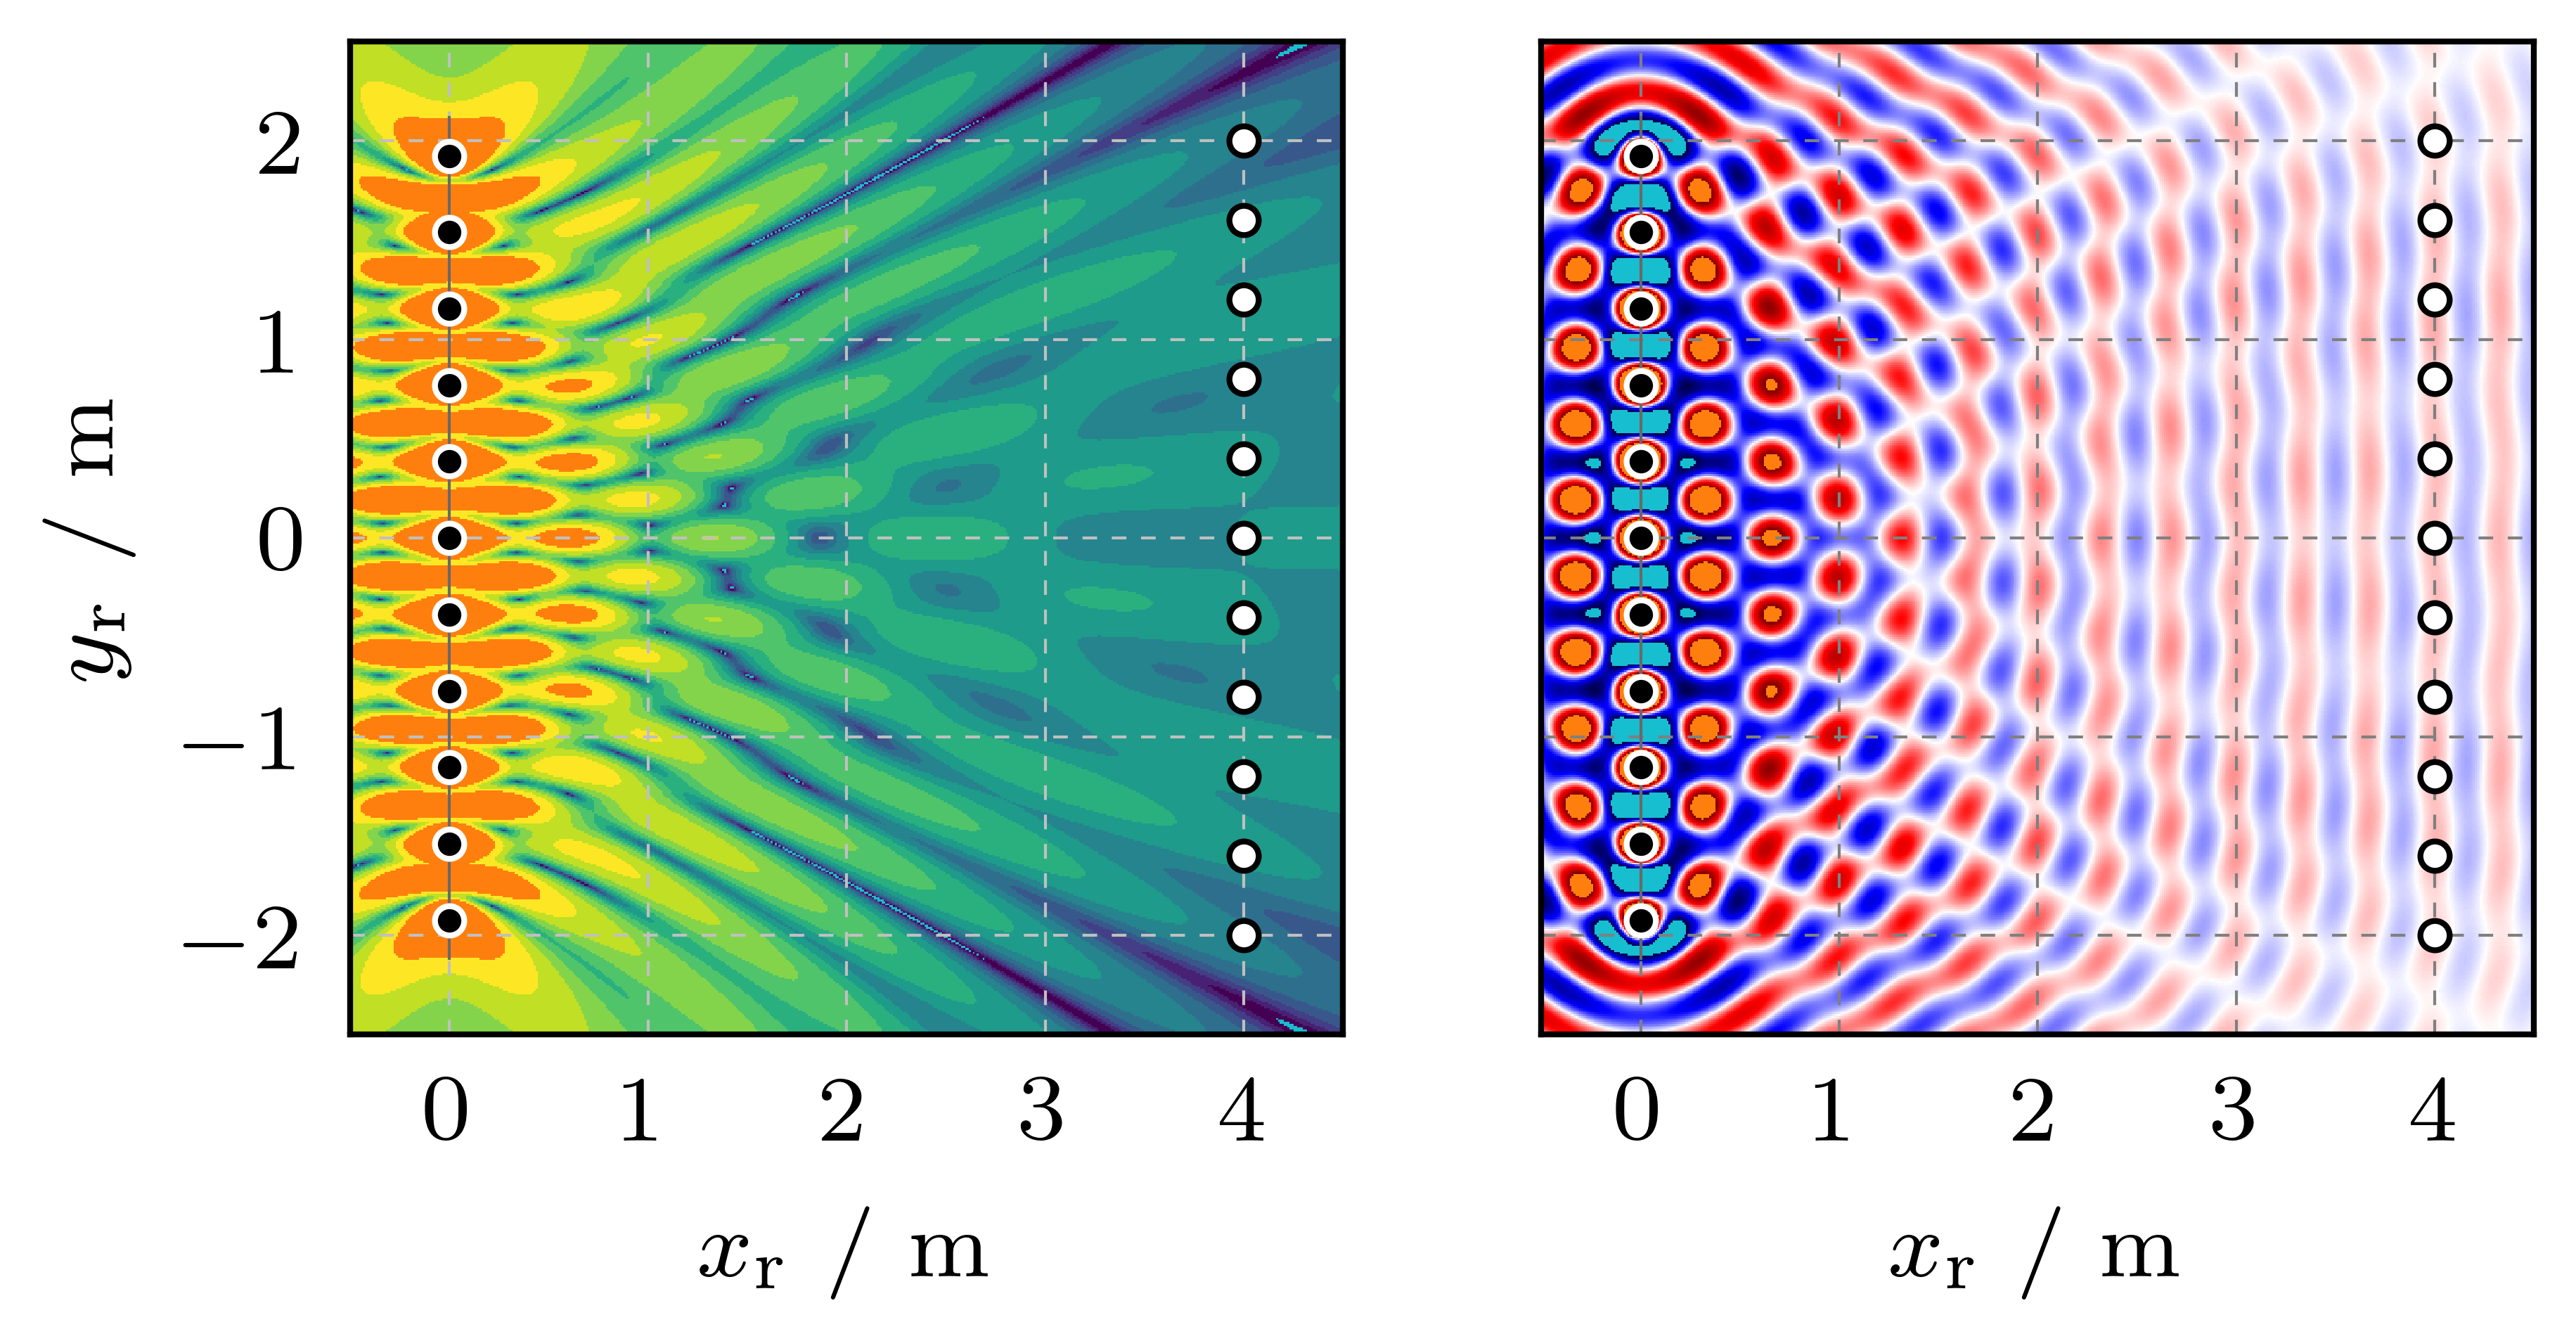
\includegraphics[width=85mm]{../python/wfs25d_lineSSD_aliasing.png}
\end{plotfigures}
\caption{2.5D-WFS einer virtuellen Punktquelle bei
$\xp = (-100,0,0)^\mathrm{T}$\,m mit 11 Monopolen entlang der $y$-Achse
(schwarze Punkte, Abstand $\Delta_{\xs}\approx 0{,}3849$\,m)
für die Wellenlänge $\lambda=\frac{1}{3}$\,m.
%
2.5D-WFS-Amplitudenkorrektur auf $0$\,dB-Pegel entlang der Referenzlinie bei
$x=4$\,m.
%
Die 11 weißen Punkte auf dieser bilden mit den 11 Monopolen jeweils ein
Punktpaar mit stationärer Phasenbedingung.
%
Zusätzlich zur Beugung tritt räumliches Aliasing wegen zu großem Lautsprecherabstand
$\Delta_{\xs} $ auf:
vor allem die Wellenanteile mit hohem Pegel und
Ausbreitungsrichtungen um $\pm 60^\circ$ beeinträchtigen die
gewünschte ebene $0^\circ$-Wellenfront im Nahfeld des Arrays.
%
Im Fernfeld des Arrays bildet sich die Richtcharakteristik
\Abb\ref{fig:wfs25d_lineSSD_polar_plot_overlay}~(rechts) aus.
%
\cc
}
\label{fig:wfs25d_lineSSD_aliasing}
\end{figure}
%
Gemäß des räumlichen Abtastkriteriums\index{Abtastkriterium, räumlich},
vgl. \cite[Kap.~26.4]{Skudrzyk1971}, wird räumliches Aliasing\index{Aliasing, räumlich}
in der Wellenfront vollständig vermieden, wenn für die höchste im Ansteuerungssignal
vorkommende Frequenz $f_\text{max}$ der hüllkonturspezifische Abstand
$\Delta_{\xs}$
\begin{align}
\label{eq:SamplingCriterion}
\Delta_{\xs} < \frac{c}{2 f_\text{max}}\quad\leftrightarrow\quad
\Delta_{\xs} < \frac{\lambda_\text{min}}{2}
\end{align}
zwischen zwei Lautsprechern eingehalten wird, vgl. \cite[S.~246]{Stenzel1927},
\cite[Kap.~4]{Winter2019_diss}.
%
Im Falle eines linearen Arrays entspricht $\Delta_{\xs}$ direkt dem
Lautsprecherabstand.
%
Für konvexe Arrays gilt dieses harte Kriterium als sehr gute Näherung;
im Fall des dichtbepackten Kreisarrays kann die Kreisbogenlänge zwischen
zwei benachbarten Lautsprechern für $\Delta_{\xs}$ verwendet werden.
%
Für die oberen 3--4 Oktaven des menschlichen Hörvermögens bedingt
die \Glg\eqref{eq:SamplingCriterion}
erheblichen Hardwareaufwand wegen der erforderlichen sehr kleinen
Lautsprecherabstände.
%
Bei praxisnahen WFS-Systemen mit typischen Lautsprecherabständen zwischen
$0{,}1 \dots 0{,}25\,\text{m}$ tritt räumliches Aliasing bei Frequenzen oberhalb
$1715 \dots 686\,\text{Hz}$
auf.
%
Im Beispiel von \Abb\ref{fig:wfs25d_lineSSD_aliasing} wird die
\Glg\eqref{eq:SamplingCriterion}
wegen
$\Delta_{\xs}\approx 0{,}3849\,\text{m} > \frac{\lambda}{2}=\frac{1}{6}\,\text{m}$
verletzt.
%
Artefakte von räumlichem Aliasing entstehen durch Wellenfronten anderer
Ausbreitungsrichtungen, die mit der gewünschten, hier ebenen $0^\circ$-Wellenfront
interferieren.
%
Die frequenzabhängige Anzahl und Ausbreitungsrichtung(en) der
Aliasing-Wellenfronten,
vgl. \cite{Stenzel1927,Berkhout1993_JASA,Start1997_diss, Winter2019_diss},
lässt sich u.a. aus der
Fernfeldrichtcharakteristik in
\Abb\ref{fig:wfs25d_lineSSD_polar_plot_overlay}~(rechts) bestimmen.
%
Im Beispiel sind es die beiden sogenannten Gitterkeulen
bei exakt $\pm 60^\circ$,
welche bei Benutzung von omnidirektional abstrahlenden
Monopol-Sekundärquellen
den gleichen Pegel wie die $0^\circ$-Hauptkeule
aufweisen.
%
Das Schallfeld ist im Nahfeld erst in einiger Entfernung zum endlichen Array
näherungsweise aliasing-frei, im Beispiel gilt das bei der gewählten Frequenz
grob jenseits der Referenzlinie bei $x=4$\,m mittig vor dem Array.
%
%Je kleiner der Abstrahlwinkel der Gitterkeulen ist, desto größer der Bereich
%im Nahfeld in dem das Schallfeld Aliasingartefakte aufweist.



In \Abb\ref{fig:wfs25d_circSSD_aliasing} ist ein weiteres aliasing-behaftetes
Schallfeld dargestellt, bedingt durch ein räumlich diskretisiertes,
kreisförmiges Array.
%
% please DO NOT rescale the figure and keep it single column
\begin{figure}[t]
\centering
\begin{plotfigures}
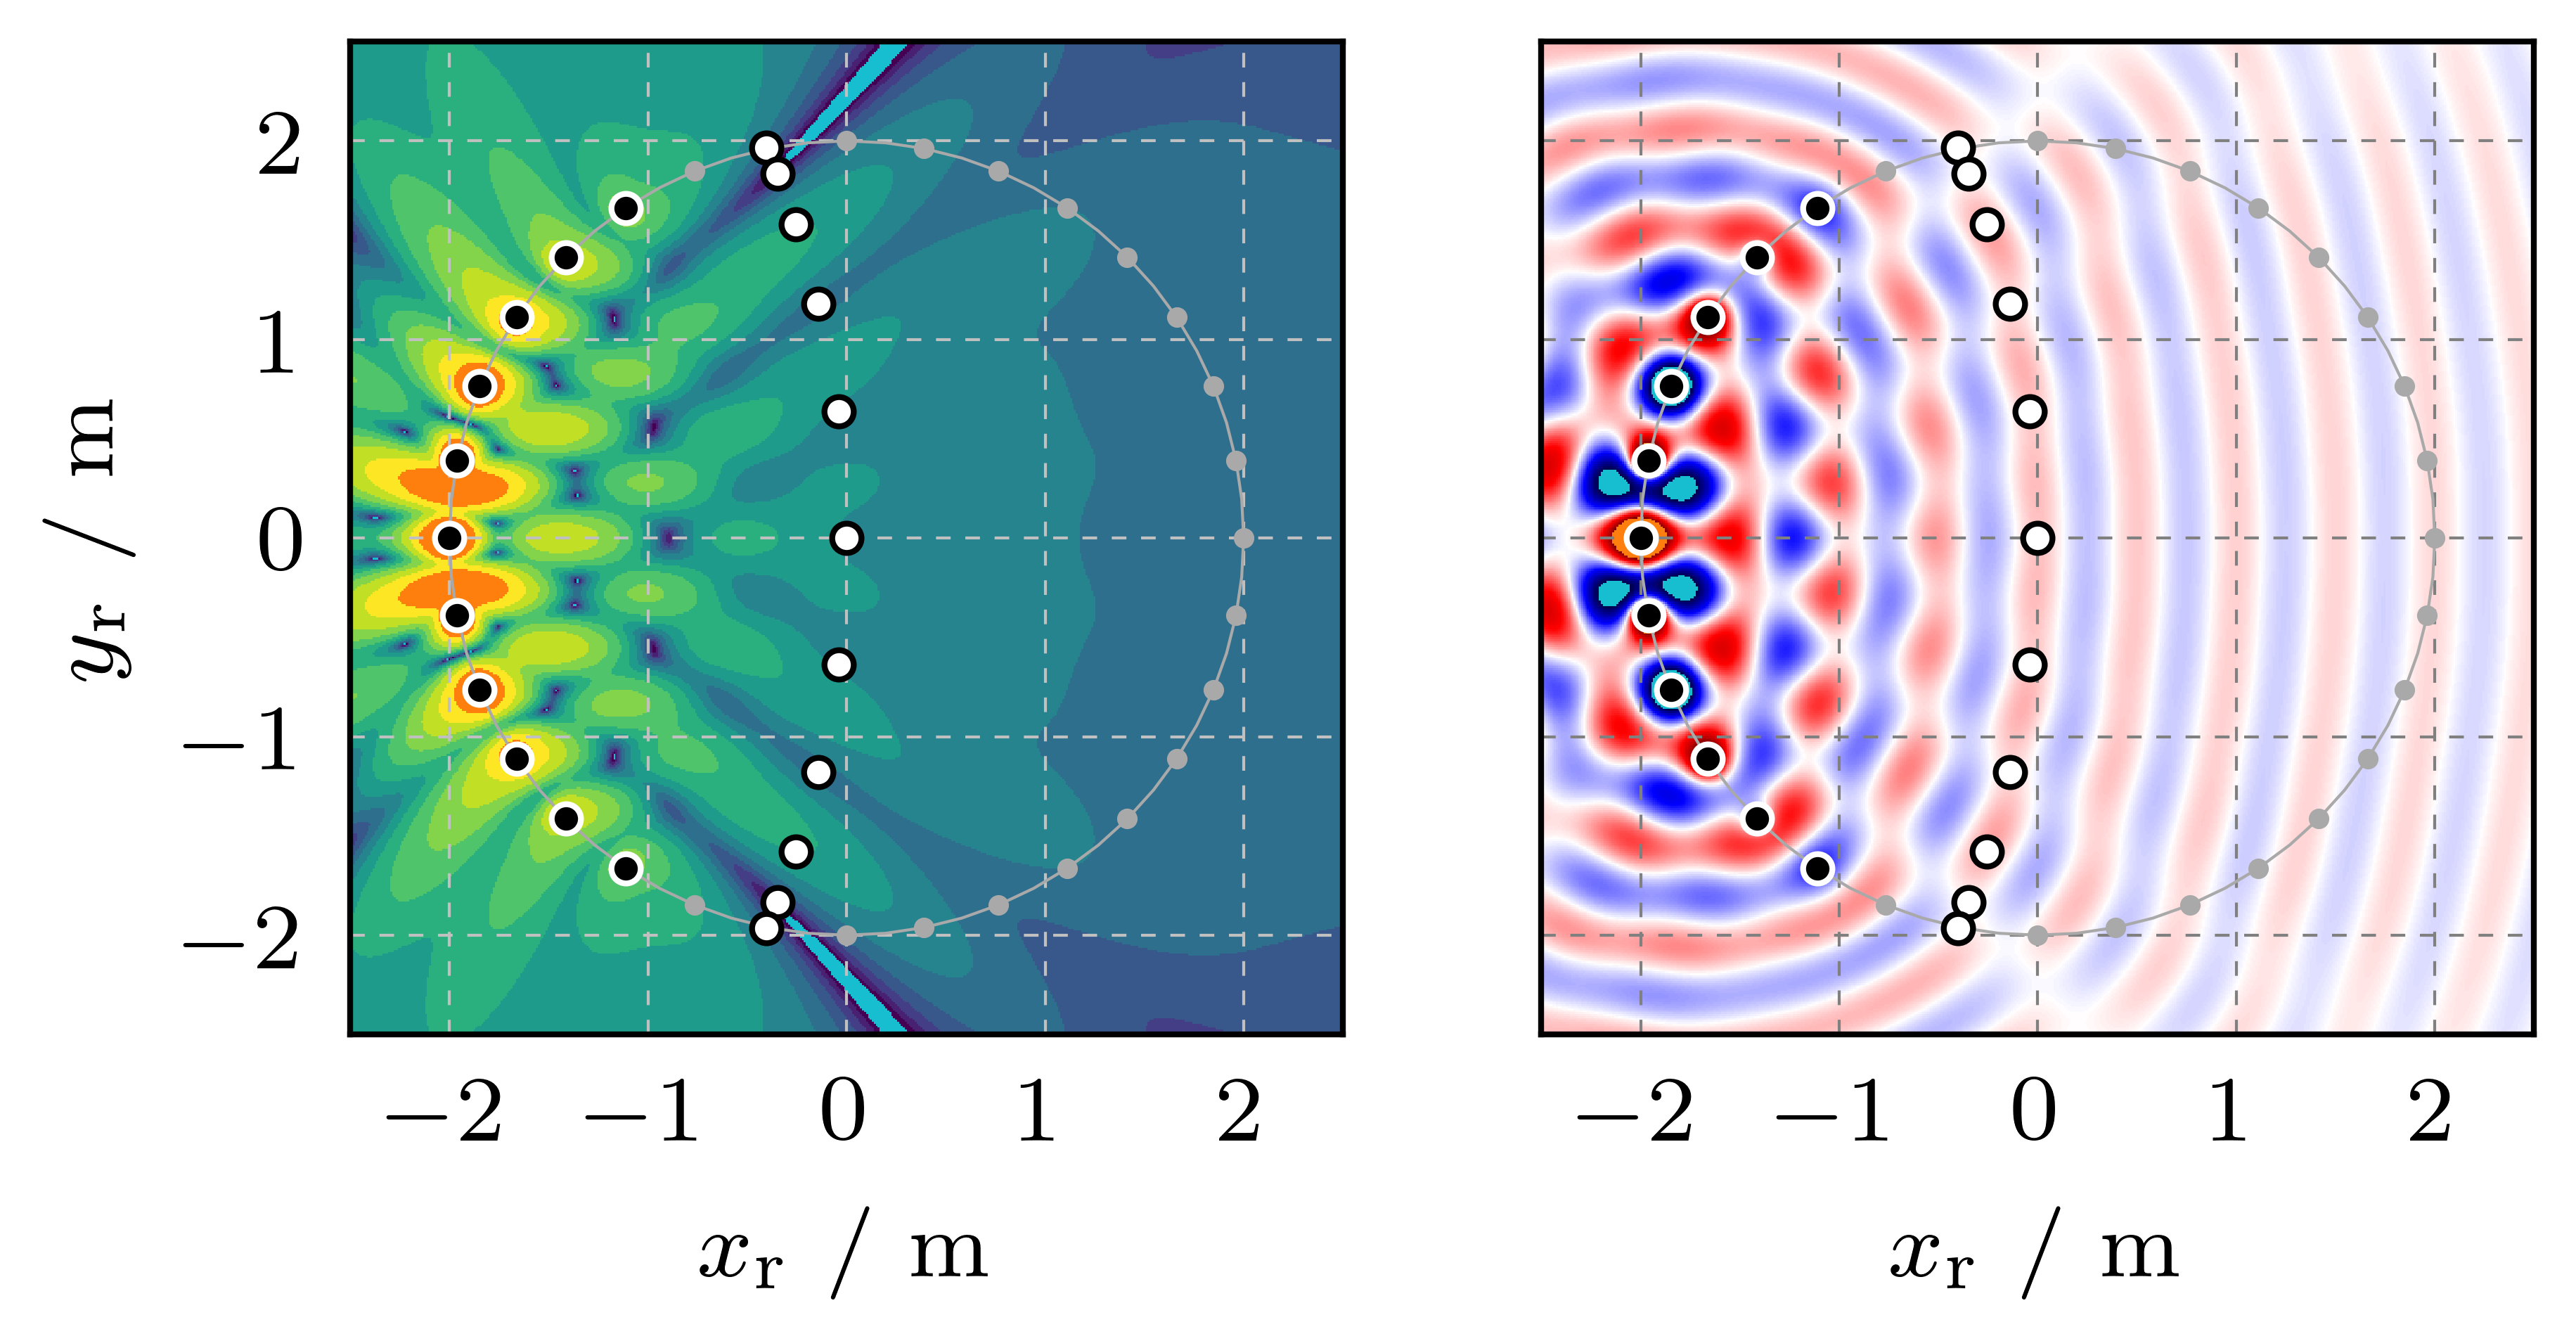
\includegraphics[width=85mm]{../python/wfs25d_circSSD_aliasing.png}
\end{plotfigures}
\caption{2.5D-WFS einer virtuellen Punktquelle bei $\xp = (-5,0,0)^\mathrm{T}$\,m
mit 32 äquiangular verteilten Monopolen auf einem 2\,m-Radius-Kreisarray
für die Wellenlänge $\lambda=\frac{1}{2}$\,m.
%
2.5D-WFS-Amplitudenkorrektur auf $0$\,dB-Pegel entlang des mittigen Kreisbogens.
%
Die 11 weißen Punkte auf diesem Kreisbogen bilden mit den 11 aktiven Monopolen
(schwarze Punkte) jeweils ein Punktpaar mit stationärer Phasenbedingung.
%
Bei der, zur sinnvollen Veranschaulichung, gewählten Frequenz gilt speziell, dass
im linken bzw. rechten Teil der kreisförmigen Zuhörerfläche viel bzw. wenig
Aliasingartefakte die gewünschte Wellenfront beeinträchtigen.
%
\cc
}
\label{fig:wfs25d_circSSD_aliasing}
\end{figure}
%
Für den gewählten Radius ist die Verwendung von 32 bis 64 Lautsprechern
praxisnah.
%
Für die gewünschte gekrümmte Wellenfront einer virtuellen Punktquelle
ist räumliches Aliasing rechts der gewählten Kreisbogen-Referenzkurve
bei der gewählten Frequenz annähernd vernachlässigbar.
%
Für die betrachtete Frequenz enthält das Schallfeld links der Referenzkurve,
also näher an den aktiven Monopolen, deutlich Aliasingartefakte.



Während sich für planare, lineare, sphärische und zirkuläre Arrays
die Entstehung räumlichen Aliasings mittels räumlicher Fourier-Transformation
vergleichsweise bequem studieren lässt,
vgl. \cite{Start1997_diss,Spors2008b,Ahrens2010_IEEE,Fazi2010,Schultz2016_diss},
ist vor allem für kompliziertere Geometrien und damit einhergehend fehlender
analytischer Lösungen ein akustisches Strahlenmodell\index{Schallstrahlenmodell}
nützlich, vgl. \cite{Winter2019_diss}.
%
Dies kann vorteilhaft genutzt werden, um aliasing-freie Zonen über einen großen
Frequenzbereich näherungsweise zu prädizieren ohne aufwändige Simulationen von
Schallfeldern und Richtcharakteristiken durchführen zu müssen.



\subsection{Impulsartiges Schallfeld}
%
% please DO NOT rescale the figure and keep it double column
\begin{figure*}[t]
\centering
\begin{plotfigures}
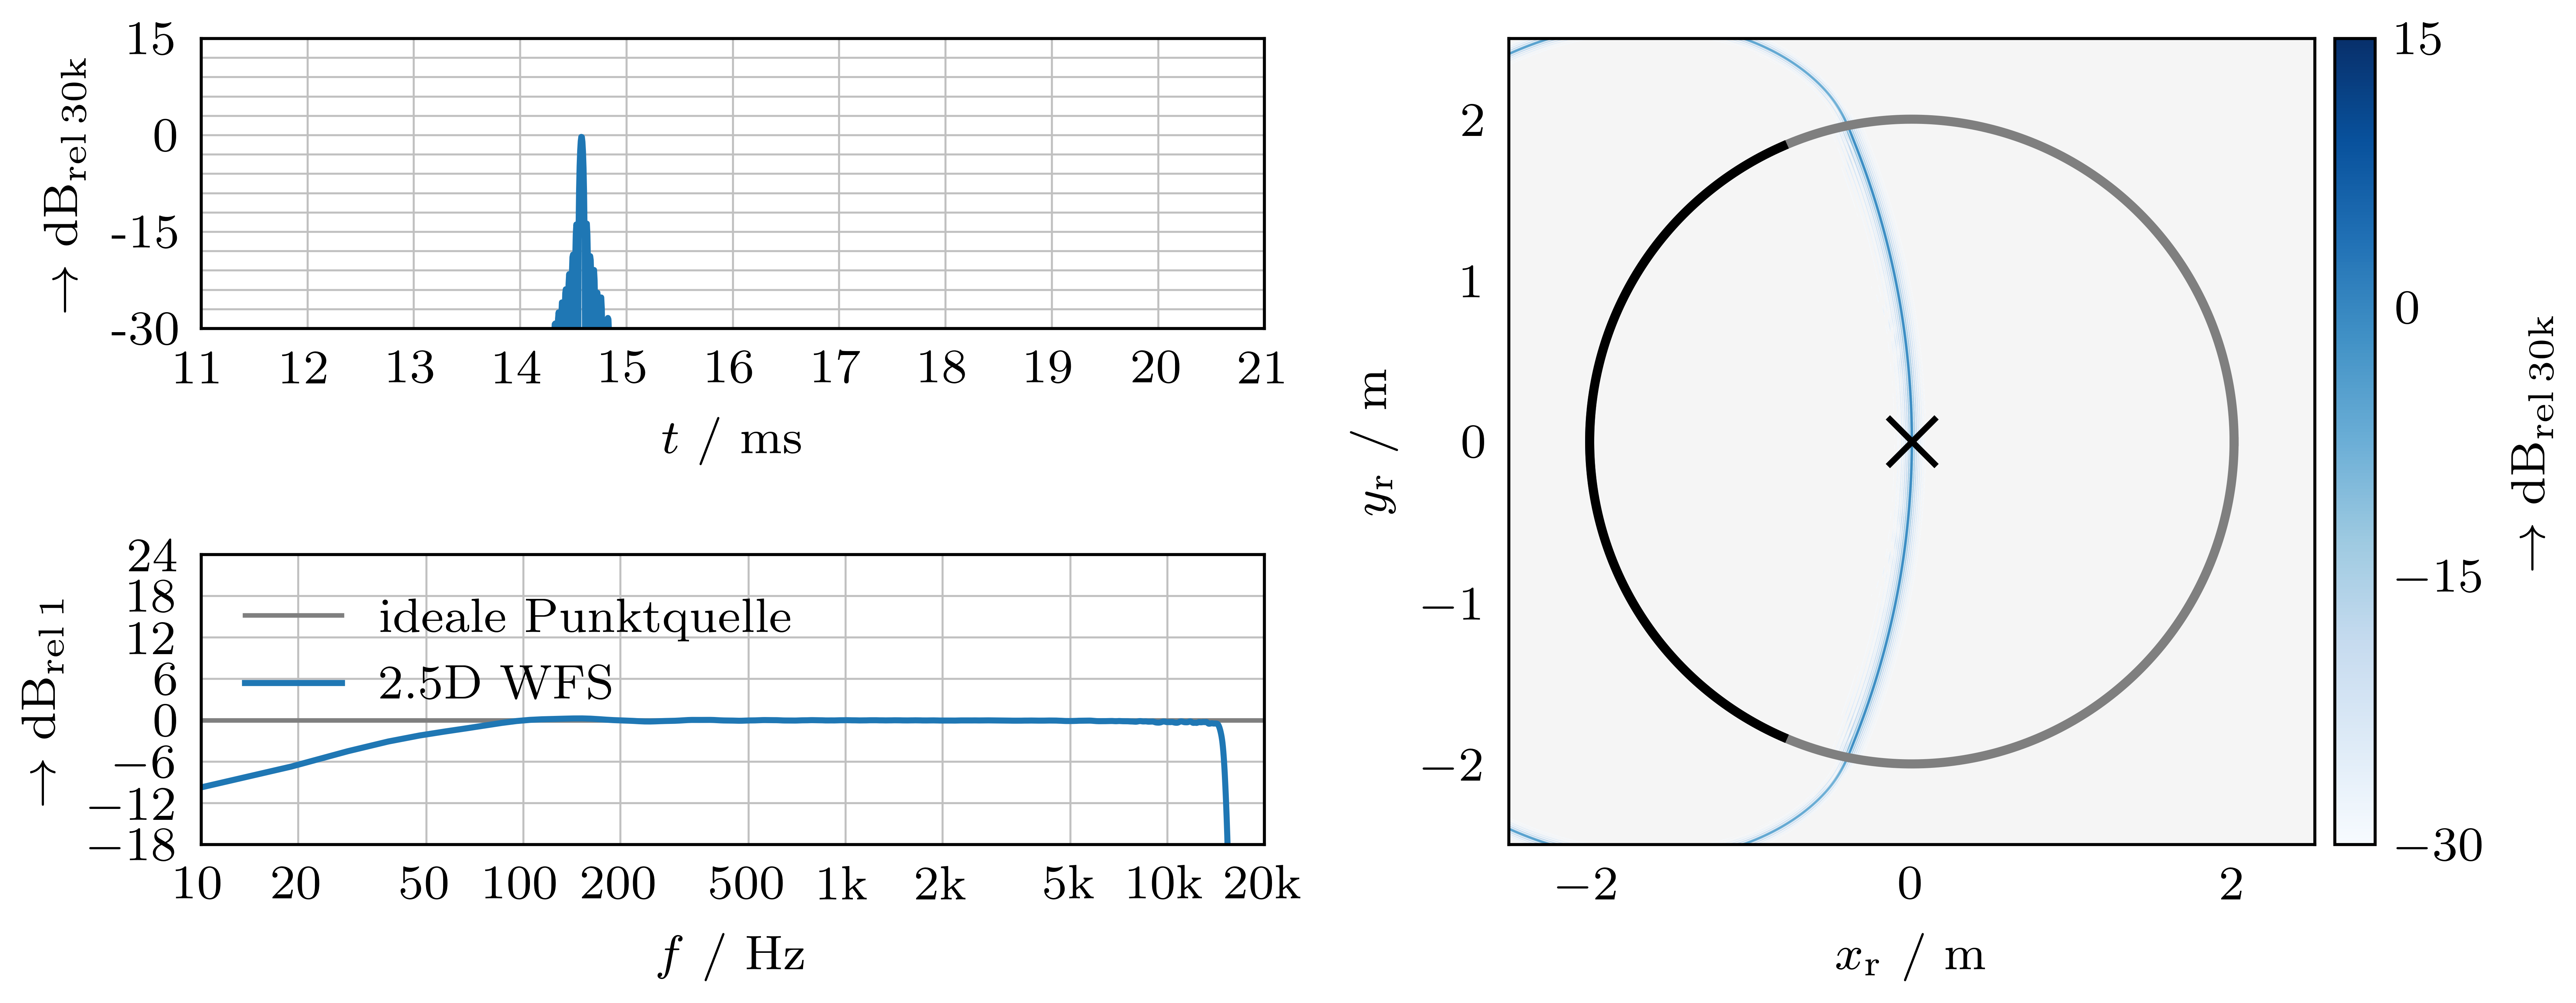
\includegraphics[width=145mm]{../python/wfs25d_circSSD_noaliasing_time_domain_x0.00_m_py_DEU.png}
\end{plotfigures}
\caption{2.5D-WFS-Schallfeld bei impulshafter Anregung zum Zeitpunkt $t=0$\,s
(rechts) für das Szenario aus \Abb\ref{fig:wfs25d_circSSD_aliasing}, allerdings
hier mit kontinuierlichem Kreisarray, aktiver Teil des Arrays in schwarz,
inaktiver Teil in grau.
%
Hier und in \Abb\ref{fig:td_-1m} bis \ref{fig:td_1m} gilt für die
rechte Grafik des impulshaften Schallfelds:
%
Pegel $>+15\,\text{dB}$ erfahren eine Farbsättigung mit schwarz,
Pegel $<-30\,\text{dB}$ hingegen mit grau.
%
Der dargestellte Zeitpunkt $t \approx 14{,}578$\,ms entspricht der
Schallausbreitungszeit der virtuellen Punktquelle zum Messpunkt $\times$ bei
$\xr=(0,0,0)^\mathrm{T}$\,m für die Schallgeschwindigkeit $c=343$\,m/s.
%
Akustische Impulsantwort (links, oben) und Frequenzgang (links, unten)
am Messpunkt $\times$.
%
Die perfekt synthetisierte Wellenfront ist koinzident mit der Referenzkurve,
daher im Frequenzgang gewünschter $0$\,dB-Referenzpegel
zwischen ca. $100$\,Hz und $15$\,kHz.
%
Impulsspezifischer Pegel in $\text{dB}_{\text{rel }30\text{k}}$ relativ zum
endlichen Amplitudenwert $30{.}000$ des zeitkontinuierlichen, $15$\,kHz-tiefpassbegrenzten Anregeimpulses.
%
\cc
}
\label{fig:td_0m_noaliasing}
\end{figure*}
%
Die
%fig:td_0m_noaliasing %Abb.~\ref{fig:td_-1m},~\ref{fig:td_0m},~\ref{fig:td_1m}
\Abb\ref{fig:td_0m_noaliasing} bis \ref{fig:td_1m}
zeigen wie sich die 2.5D-WFS bei impulshafter Audiosignal-Anregung unter Benutzung
des theoretischen WFS-Vorfilters in \Glg\eqref{eq:Prefilter25D} verhält.
%
Die virtuelle Punktquelle wird zum Zeitpunkt
$t=0$\,s mit einem auf $15$\,kHz tiefpassbegrenzten, zeitlichen Dirac-Impuls angeregt,
welcher sich im Freifeld räumlich mit Schallgeschwindigkeit $c=343$\,m/s
auf eine immer größer werdende Kugelfläche ausbreitet, also ein Monopol-Schallfeld mit
$15$\,kHz-Bandbreite darstellt.
%
Für die Synthese dieser 3D-Wellenfront mit einem räumlich diskretisierten 2D-Array
und der 2.5D-Filter-Impulsantwort in \Glg\eqref{eq:h25d_time}
sind ähnliche Artefakte wie bei monofrequenter Ansteuerung zu erwarten:
a) 2.5D charakteristische Amplitudenabnahme
über den Ausbreitungsweg,
b) frequenzabhängiger Nah-/Fernfeldübergang und
c) frequenzabhängiges räumliches Aliasing.
%
\Abb\ref{fig:td_0m_noaliasing} bis \ref{fig:td_1m} zeigen
jeweils rechts die impulshafte Wellenfront in der $xy$-Ebene zu einem
bestimmten Ausbreitungszeitpunkt,
jeweils links/oben die Antwort des akustischen Systems auf den tiefpassbegrenzten,
zeitlichen Eingangsimpuls, die mit einem Messmikrofon am Aufpunkt $\times$ gemessen
würde und
jeweils links/unten den zugehörigen Frequenzgang.
%
%Die Simulationen erfolgten mit Abtastfrequenz $f_s = 192$\,kHz.



\Abb\ref{fig:td_0m_noaliasing} zeigt das Ergebnis einer Simulation mit einem
kontinuierlichen Kreisarray.
%
Es treten daher nur die Artefakte der Punkte a) und b) auf.
%
Für den Frequenzbereich $100\,\text{Hz} < f < 15\,\text{kHz}$
wird eine nahezu perfekte Wellenfront synthetisiert.
%
Zum dargestellten Zeitpunkt ist die Wellenfront koinzident mit der gewählten
Referenzkurve.
%
Der Frequenzgang entspricht daher dem gewünschten $0$\,dB-Referenzpegel in diesem
Frequenzbereich.
%
Unterhalb $100$\,Hz tritt Hochpassverhalten auf.
%
In diesem Beispiel sind dafür zwei Aspekte konfundiert verantwortlich.
%
Zum einen sind für kleiner werdende Frequenzen
die zugehörigen Wellenlängen zunehmend größer als die Apertur\index{Apertur}.
%
Das Array bietet für diese Wellenlängen keine Kontrolle von Interferenz
in einem ausgedehnten Nahfeld, es strahlt in vergleichsweise naher Entfernung
schon ins Fernfeld ab.
%
Zum anderen gilt die Fernfeld-/Hochfrequenznäherung $\wc r_{\xs\text{-}\xr} \gg 1$
für die tiefen Frequenzen und den gewählten Aufpunkt nicht.
%
Es ist also zu erwarten, dass die tatsächliche physikalische Synthese von der
gewünschten WFS-Lösung abweicht.



\Abb\ref{fig:td_-1m} bis \ref{fig:td_1m} entsprechen dem Szenario aus
\Abb\ref{fig:wfs25d_circSSD_aliasing}, d.h. einem räumlich diskretisierten
Kreisarray mit 32 Monopolen.
%
Durch die räumliche Diskretisierung des Arrays entstehen für $f>f_\text{max}$
räumliche Aliasingartefakte, die in den drei Darstellungen unterschiedlich
repräsentiert werden: entweder als nicht geschlossene Wellenfront bzw.
als eine Wellenfronteinhüllende (rechts),
als zeitliche Folge von Impulsen (links/oben, im Folgenden wegen der
Tiefpassbegrenzung technisch zwar ungenau aber wesentlich korrekt als
Impulsantwort bezeichnet) oder als hochfrequente Frequenzgangsverzerrungen
(links/unten).



Insgesamt sind wie auch in \Abb\ref{fig:wfs25d_circSSD_aliasing} elf Monopole, die
Lautsprecher (LS) 12--22, gemäß des \textit{secondary source selection criterion}
nach \Glg\eqref{eq:SecSrcSel} an der Synthese beteiligt und definieren die Apertur.
%
Die anderen Lautsprecher werden für die gewählte Parametrik der virtuellen Quelle
nicht benötigt und daher nicht angesteuert.
%
In den Impulsantworten dieses 2.5D-WFS-Szenarios lässt sich immer eine Abfolge von
sechs Impulsen in der Impulsantwort erkennen.
%
Der erste stammt von LS 17.
%
Dieser befindet sich auf der $x$-Achse in Linie mit der
Primärquellenposition und allen drei gezeigten Messpunkten, ist für diese also
genau der Monopol mit stationärer Phasenbedingung und weist die kürzeste
Distanz zur virtuellen Quelle auf.
%
Es folgen zeitlich fünf Impulse nach, die den, wegen des Delays in der
Treiberfunktion, verzögert spielenden Monopolen zuordenbar sind.
%
Der zweite Impuls wird demzufolge von den LS 16 und 18 zu exakt gleichen
Anteilen erzeugt und hat höhere Amplitude als der Erstimpuls.
%
Der letzte Impuls stammt entsprechend von LS 12 und 22.
%
Diese paarweise Koinzidenz entsteht durch die gewählte Geometrie:
%
das Array ist symmetrisch zur $x_\mathrm{r}$-Achse, auf der wie
erwähnt auch die Primärquelle und die Messpunkte positioniert sind.
%
Das sechsfach Impulsmuster ist also für alle Messpunkte auf der
horizontalen Symmetrieachse gleich, allerdings ändern sich über die
Entfernung vom aktiven Array die relativen Zeitbezüge der Impulse.
%
Der Erstimpuls hingegen lässt sich zeitlich immer exakt bezüglich der
Schallgeschwindigkeit $c$ und Position der virtuellen Punktquelle
verorten.
%
Die resultierenden, zeitlich nichtkompakten Impulsantworten repräsentieren
räumliches Aliasing im Zeitbereich.
%
%
%
% ##############################################################################
% try to render these 3 figures on a single page such that readers can
%  conveniently compare them
% this might also work as subplot figure a,b,c ?!?!
% please DO NOT rescale the figure and keep it double column
\begin{figure*}[t]
\centering
\begin{plotfigures}
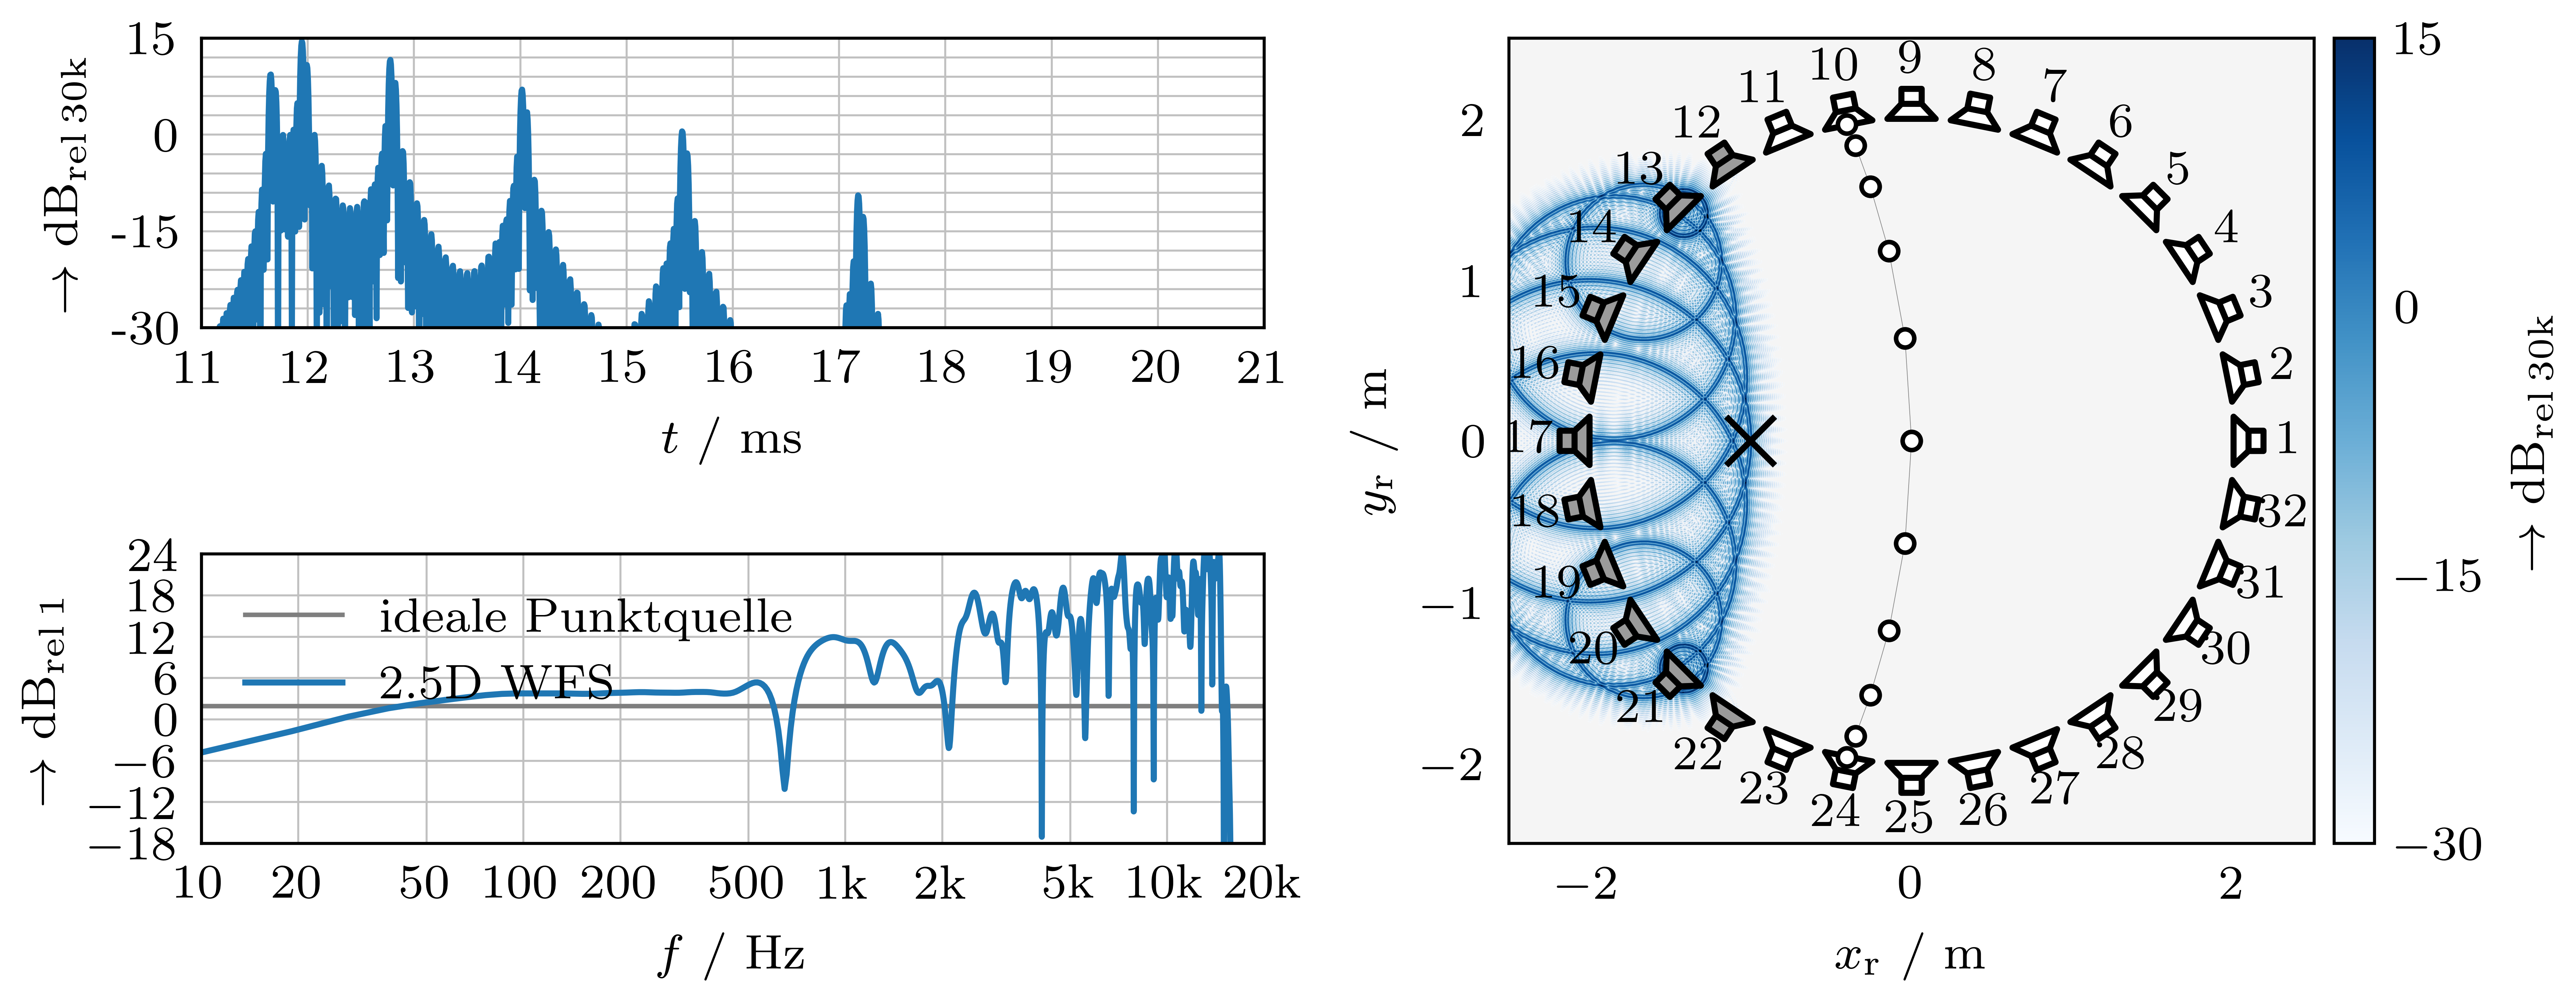
\includegraphics[width=145mm]{../python/wfs25d_circSSD_aliasing_time_domain_x-1.00_m_py_DEU.png}
\end{plotfigures}
\caption{2.5D-WFS-Schallfeld (rechts) bei impulshafter Anregung zu $t=0$\,s für das
Szenario aus \Abb\ref{fig:wfs25d_circSSD_aliasing}.
%
Pegelreferenzkurve als Kreisbogen durch $\xr=(0,0,0)^\mathrm{T}$\,m (rechts).
%
Dargestellter Zeitpunkt $t\approx 11{,}662$\,ms bei Schallgeschwindigkeit
$c=343$\,m/s entspricht der Wellenlaufzeit der virtuellen Punktquelle zum
Messpunkt $\times$ bei $\xr=(-1,0,0)^\mathrm{T}$\,m.
%
Akustische Impulsantwort (links, oben) und Frequenzgang (links, unten) vom Messpunkt $\times$.
%
\cc
}
\label{fig:td_-1m}
\end{figure*}
%
%
%
% please DO NOT rescale the figure and keep it double column
\begin{figure*}[h!]
\centering
\begin{plotfigures}
\includegraphics[width=145mm]{../python/wfs25d_circSSD_aliasing_time_domain_x0.00_m_py_DEU.png}
\end{plotfigures}
\caption{2.5D-WFS-Schallfeld
ähnlich \Abb\ref{fig:td_-1m} für Zeitpunkt $t \approx 14{,}578$\,ms,
Messpunkt $\times$ bei $\xr=(0,0,0)^\mathrm{T}$\,m.
%
Wellenfront ist koinzident mit der Pegelreferenzkurve, daher
%
im Frequenzgang gewünschter (aliasing-freier) $0$\,dB-Referenzpegel zwischen ca. $100$ und $600$\,Hz.
%
\cc
}
\label{fig:td_0m}
\end{figure*}
%
%
%
% please DO NOT rescale the figure and keep it double column
\begin{figure*}[h!]
\centering
\begin{plotfigures}
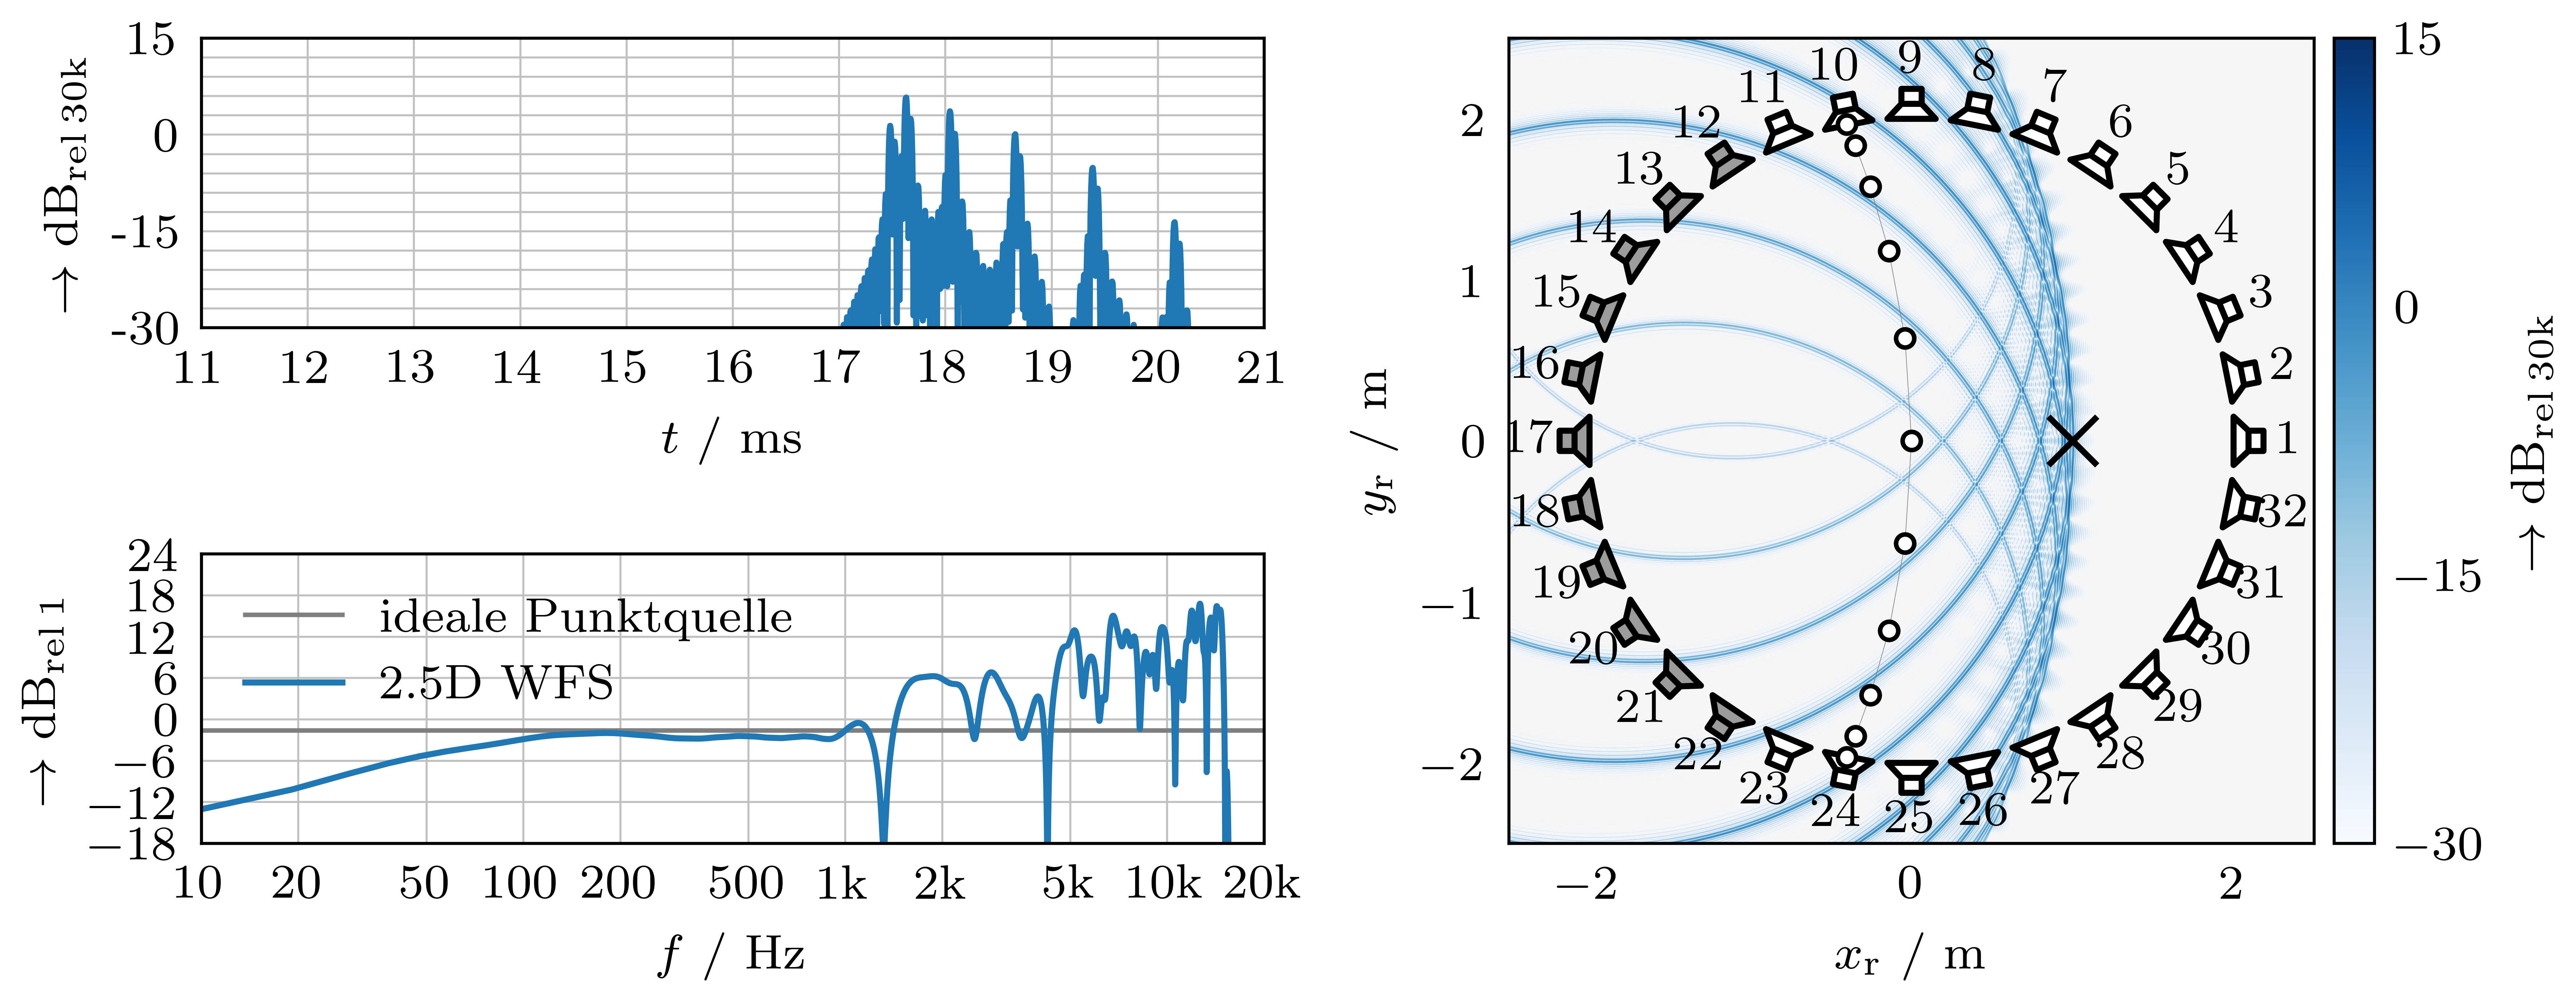
\includegraphics[width=145mm]{../python/wfs25d_circSSD_aliasing_time_domain_x1.00_m_py_DEU.png}
\end{plotfigures}
\caption{2.5D-WFS-Schallfeld
ähnlich \Abb\ref{fig:td_-1m} für Zeitpunkt $t \approx 17{,}493$\,ms,
Messpunkt $\times$ bei $\xr=(1,0,0)^\mathrm{T}$\,m.
%
\cc
}
\label{fig:td_1m}
\end{figure*}
% try to render the above 3 figures on a single page for convenient comparison
% ##############################################################################



Räumliches Aliasing aus Sicht der zugehörigen Spektren offenbart
hochfrequent stark positionsabhängige Abweichungen vom gewünschten linearen
Frequenzgang.
%
Das für ein Kreisarray näherungsweise geltende Kriterium nach \Glg\eqref{eq:SamplingCriterion} zur vollständigen
Vermeidung von Aliasing
führt mit der Kreisbogenlänge
$\Delta_{\xs}=0{,}3927$\,m zur Grenzfrequenz
$f_\text{max} = \frac{c}{2 \Delta_{\xs}}\approx 437$\,Hz,
% 343 / (2 * (2 * pi * 360/2^5 / 180))
oberhalb derer Aliasingartefakte im Frequenzgang zu erwarten sind.
%
Tatsächlich ist die Frequenz $f_\text{al}$ ab der Aliasing auftritt,
vom Messpunkt und der Array-Geometrie abhängig, und
kann $f_\text{al}>f_\text{max}$, aber niemals $f_\text{al}<f_\text{max}$ sein.
%
Dies lässt sich verknüpfen mit der obigen Beobachtung: das Schallfeld
weist für mittig vom Array entferntere Messpunkte (höhere $f_\text{al}$) geringere
Aliasingartefakte auf, als nähere Messpunkte (niedrigere $f_\text{al}$).
%
Charakteristisch für Aliasingartefakte
im Frequenzgang sind a) zahlreiche Anti-Resonanzen (Notches) und Resonanzen,
deren spektrale Lage von der Messposition abhängt und
b) eine steigende Flanke mit $+3$\,dB/Oktave,
vgl. \cite{Spors2010a}.
%
Dies wird typisch als Klangverfärbung (\textit{colouration})
wahrgenommen, vgl. \cite{Start1997_diss, Wittek2007_JAES, Wierstorf2014_diss, Winter2019_diss, Erbes2020_diss}.
%
Es wird speziell dann sehr deutlich als sogenanntes Phasing wahrgenommen,
wenn sich der Frequenzgang über die Zeit sehr stark ändert, etwa weil sich
virtuelle Quelle und/oder Zuhörende (schnell) bewegen.
%
Der Frequenzgang der drei Beispiele ist zwischen ca. $100$ und $600$\,Hz
annähernd linear und variiert über die Messpunkte mit der charakteristischen
2.5D-Amplitudenabnahme der virtuellen Punktquelle bezogen auf den
$0$\,dB-Referenzpegel in \Abb\ref{fig:td_0m}.
%
Das Hochpassverhalten unterhalb $100$\,Hz wurde bereits für
\Abb\ref{fig:td_0m_noaliasing} beim kontinuierlichen Array diskutiert,
es sind die selben Phänomene.


Die durch räumliches Aliasing entstehenden starken Frequenzgangsverzerrungen
sollten im perzeptiven Kontext relativiert werden.
%
Ein 2.5D-WFS System mit praktikablem $17$\,cm-Lautsprecherabstand
wurde beispielsweise weniger klangverfärbend wahrgenommen als
Off-Center Stereo-Wiedergabe; und bei Sprache führt dieses WFS-Setup und On-Center
Stereo-Wiedergabe zur ungefähr gleich wahrgenommenen
Klangverfärbung \cite{Wierstorf2014_diss}.
%
Für breitbandige Signale, die vergleichsweise viel räumliches Aliasing anregen,
führen Raumreflexionen zur Glättung des Frequenzgangs, was verglichen mit dem
Freifeldfall perzeptiv in weniger Klangverfärbung münden kann \cite{Erbes2020_diss}.



Räumliches Aliasing aus Sicht der Wellenfront ist anschaulich
in \Abb\ref{fig:td_-1m} bis \ref{fig:td_1m}~(jeweils rechts)
dargestellt.
%
Die gewünschte Wellenfrontkrümmung wird korrekt synthetisiert, jedoch wird die
Wellenfront nur als Einhüllende abzählbarer Impuls-Wellenfronten erzeugt.
%
Diese Impuls-Wellenfronten korrespondieren, wenn sie an den entsprechenden
Messpunkten ankommen, exakt mit den Einzelimpulsen in den Impulsantworten.



Die Lokalisation von virtuellen Quellen synthetisiert mit WFS erfolgt
vergleichsweise robust \cite{Start1997_diss,Wittek2007_diss,Rohr2013_JAES,Wierstorf2014_diss,Erbes2020_diss}
was mit dem Gesetz der ersten Wellenfront \cite{Blauert1997_book} erklärbar ist.
%
In den diskutierten Beispielen eilt der Schall von LS 17 zeitlich immer voraus.
%
Es gibt für alle Empfängerpunkte auf der Horizontalachse $x_\mathrm{r}$
keinen anderen Lautsprecher der näher zur virtuellen Punktquelle ist.
%
Später spielende Lautsprecher und Raumreflexionen treffen
verzögert zu diesem Erstimpuls am Ohr ein.
%
Zur robusten Beurteilung der virtuellen Schallquellenposition reicht dem
menschlichen Hörsinn der initiale Erstimpuls.
%
Diese Analyse führt erst dann zu größeren Lokalisationsfehlern, wenn das Array
sehr, sehr große Lücken zwischen den Lautsprechern aufweist und eine einzelne
von der virtuellen Schallquellenposition stark abweichende, diskrete
Lautsprecherposition für die maßgebliche Erzeugung des ersteintreffenden Impulses
verantwortlich ist.
%
Das WFS-Array ist in solch einem Fall mutmaßlich so dünn besetzt (vgl.
\textit{sparse array}), dass nicht mehr von Synthese einer geschlossenen
Wellenfront gesprochen werden sollte.
%
Die resultierenden Frequenzgangsverzerrungen führen zu
psychoakustischen Effekten
(z.B. Phantomschallquelle \cite{Blauert1997_book}), die
eher der Stereo- oder LCR-Wiedergabe zuordenbar sind,
vgl. \cite{Wittek2007_diss,Wierstorf2014_diss}.



\section{Praxisrelevante Modifikationen für 2.5D-WFS}
\label{sec:mods_25d_wfs}
%
Die 2.5D-WFS-Theorie besagt, dass ein Schallfeld entlang einer
Referenzkurve näherungsweise amplitudenkorrekt synthetisiert wird,
vgl.~\Abb\ref{fig:25DWFS_Schema}.
%
In der Praxis führen frequenzabhängige, räumliche Aliasingartefakte und
die frequenzabhängige Nah-/Fernfeldgrenze -- und damit frequenzabhängige Beugung --
zur Abweichung eines linearen Frequenzgangs wie oben diskutiert,
vgl.~\Abb\ref{fig:td_0m}.
%
Dies ist kein WFS-spezifisches Problem, sondern tritt allgemein bei allen
Wiedergabeverfahren auf, welche die physikalische
Rekonstruktion von Schallfeldern anstreben.
%
Zur Linearisierung des Frequenzgangs erfolgen typisch Anpassungen an den
theoretischen Treiberfunktionen, vgl. \cite{Apel2004,Kolundzija2009b,Spors2010a}
wovon drei Methoden nun näher diskutiert werden sollen.



\subsection{Anpassung des WFS-Vorfilters}
%
Eine sehr einfache Entzerrungsmethodik, welche bei der impliziten
Schallfeldsyntheselösung streng genommen nur einen einzelnen Empfängerpunkt
linearisiert, besteht in der Modifikation des globalen WFS-Vorfilters.
%
Dies ist beispielhaft in
\Abb\ref{fig:wfs25d_lineSSD_aliasing_eq_example} gezeigt.
%

% please DO NOT rescale the figure and keep it double column
\begin{figure*}[t]
\centering
\begin{plotfigures}
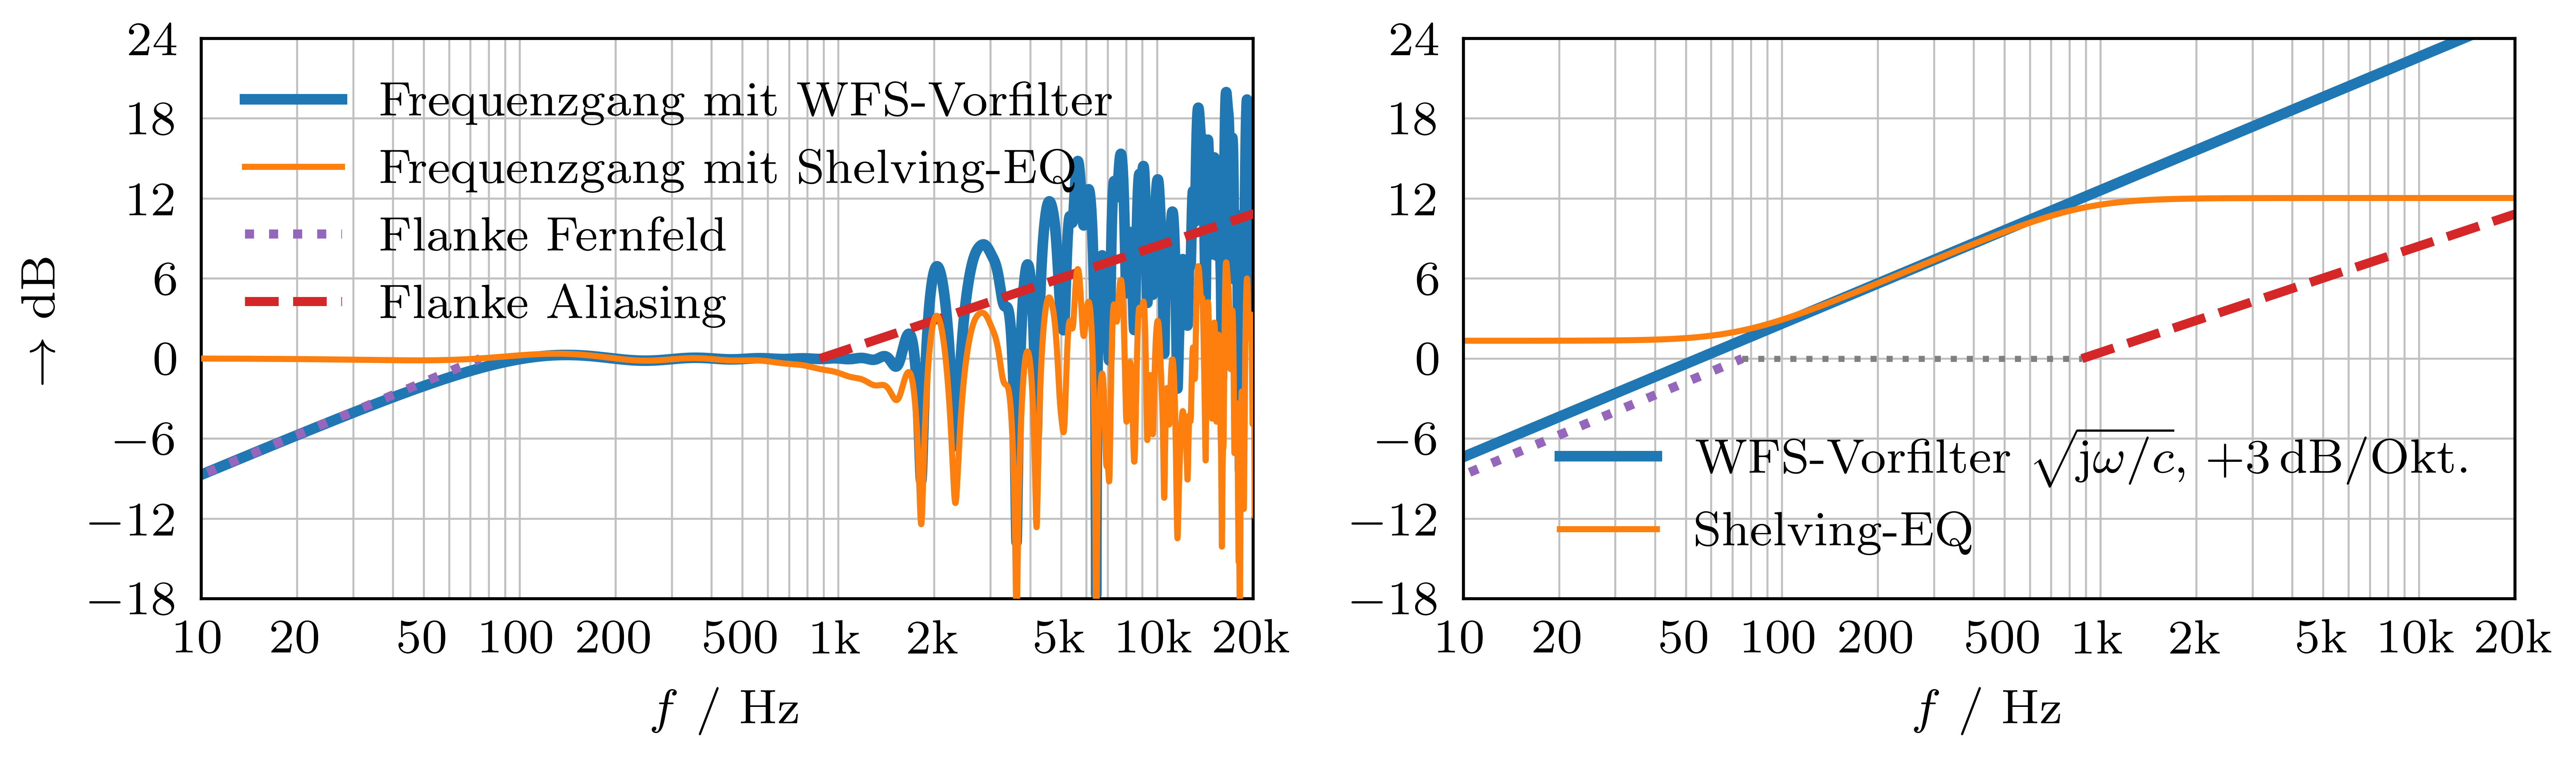
\includegraphics[width=174mm]{../python/wfs25d_lineSSD_aliasing_eq_example_DEU.png}
\end{plotfigures}
\caption{2.5D-WFS-Szenario ähnlich \Abb\ref{fig:wfs25d_circSSD_aliasing} aber
mit Kreisarray bestehend aus 64 Monopolen. Messpunkt $\xr = (0,0,0)^\mathrm{T}$\,m.
%
Frequenzgang (links, blau) unter Benutzung des theoretischen WFS-Vorfilters
$\sqrt{\im \omega/c}$ (rechts, blau).
%
Dieser gemessene Frequenzgang weist zwei charakteristische Flanken mit
ca. $+3$\,dB/Oktave auf.
%
Die tieffrequente Flanke in lila erklärt sich vor allem
durch ein zu wenig ausgeprägtes Nahfeld des Arrays (Apertur kleiner als Wellenlänge).
%
Die hochfrequente Flanke in rot erklärt sich durch den zu großen Abstand der
Monopole im Array (räumliches Aliasing).
%
Linearisierter Frequenzgang (links, orange) unter Benutzung eines
Shelving-WFS-Vorfilters (rechts, orange).
%
Die Shelving-Plateaus des Filters resultieren in einer tief- bzw. hochfrequenten
Anhebung bzw. Absenkung im Vergleich zum theoretischen WFS-Vorfilter.
%
Dies führt zu einer Linearisierung des Frequenzgangs für den gewählten Messpunkt.
%
\cc
}
\label{fig:wfs25d_lineSSD_aliasing_eq_example}
\end{figure*}
%
Dafür wurde das 2.5D-WFS-Szenario aus \Abb\ref{fig:wfs25d_circSSD_aliasing}
verwendet, jedoch mit einem Kreisarray mit 64 Monopolen, wovon 23 aktiv sind.
%
Die Kreisbogenlänge zwischen zwei Monopolen beträgt ca. $0{,}2$\,m.
%
Der gewählte Messpunkt $\xr = (0,0,0)^\mathrm{T}$\,m liegt auf der
Referenzkurve und ist Teil eines Punktpaars stationärer Phase.
%
Im Idealfall ist für diesen Messpunkt also ein linearer $0$\,dB-Frequenzgang
zu erwarten.
%
In der linken Grafik in \Abb\ref{fig:wfs25d_lineSSD_aliasing_eq_example}
ist der resultierende Frequenzgang in blau dargestellt.
%
Er weist zwei charakteristische $+3$\,dB/Oktave Flanken auf.
%
Die tieffrequente Flanke (lila) stellt das bereits diskutierte Hochpassverhalten
dar.
%
Die hochfrequente Flanke (rot) entspricht dem mittleren Pegelanstieg
durch zunehmende Ausprägung räumlichen Aliasings.
%
Da die charakteristischen (Anti)-Resonanzen stark abhängig von der
Messposition sind, lässt sich nur der mittlere Pegelanstieg sinnvoll entzerren.



Die beiden charakteristischen Flanken lassen sich mit gegenläufigen Flanken
kompensieren.
%
Die Reihenschaltung des theoretischen WFS-Vorfilters aus
der \Glg\eqref{eq:Prefilter25D} mit dem Kompensationsfilter ergibt ein für den
gewählten Messpunkt adaptiertes WFS-Vorfilter.
%
Es hat die Form eines Shelving-Filters mit $+3$\,dB/Oktave ansteigender Flanke.
%
Das Filter sollte einfach zu parametrisieren sein, da a) das WFS-Setup,
b) die Primärquellenparametrik und c) der Messpunkt einen Einfluss auf die untere
und obere Flanken-Eckfrequenz haben.
%
Diese sollten sinnvollerweise nach technischen und/oder perzeptiven
Optimierungskriterien festgelegt werden.
%
Im Beispiel wurde das Entwurfsverfahren für Shelving-Filter aus \cite{Schultz2020a}
verwendet.
%
Die obere Grenzfrequenz $f_\text{o}=f_\text{max} \approx 873$\,Hz wurde
nach dem Kriterium in \Glg\eqref{eq:SamplingCriterion} festgelegt.
%
Um den Frequenzgang am Messpunkt tieffrequent auf $\approx 0$\,dB-Pegel zu
kompensieren wurde die untere Grenzfrequenz $f_\text{u}=75$\,Hz
gewählt.
%
Der Shelving-Filter-Frequenzgang weist im Frequenzbereich $f_\text{u} < f < f_\text{o}$
die gewünschte $+3$\,dB/Oktave Flanke ähnlich des theoretischen WFS-Vorfilters auf,
vgl.~\Abb\ref{fig:wfs25d_lineSSD_aliasing_eq_example}~(rechts).
%
Für $f<f_\text{u}$ und $f>f_\text{o}$ wird der Verlauf des
theoretischen WFS-Vorfilters (blau) begrenzt und führt so zum adaptierten
Shelving-WFS-Vorfilter (orange).
%
Diese Begrenzung führt zum linearisierten Frequenzgang für den gewählten Messpunkt,
links dargestellt in \Abb\ref{fig:wfs25d_lineSSD_aliasing_eq_example} in orange.



\subsection{WFS mit numerischer Optimierung}
%
Das im vorherigen Unterabschnitt beschriebene Verfahren folgt dem
Paradigma Audiosignal-Vorfilterung, Verzögerung und Verstärkung gemäß des
Signalflusses in \Abb\ref{fig:WFS_Blockdiagramm}.
%
Es wurden WFS-Adaptionen diskutiert, welche dieses Paradigma zugunsten einer
lautsprecherindividuellen Filterung aufgeben.
%
Damit kann das Schallfeld für die jeweils gewünschte akustische Szene optimiert
werden, typisch die Minimierung von frequenzabhängigen
Beugungs- und Aliasingartefakten für einen relevanten -- meist groß intendierten
 -- Zuhörerbereich.
%
Erwähnenswert sind hier die numerischen Optimierungen
von WFS-Referenzschallfeldern \cite{Gauthier2006_JASA,Gauthier2007_JAES,Corteel2006_JAES}.
%
Diese Methoden erfordern umfangreiche Simulation und/oder Messung der
Referenzschallfelder.
%
Pro Lautsprecher wird dann ein zusätzliches Filter
mit endlicher Impulsantwort (FIR-Filter) benötigt, damit frequenzabhängig
Einfluss auf Delay und Gain genommen werden kann.
%
Im WFS-Signalflussgraphen \Abb\ref{fig:WFS_Blockdiagramm} ist dieses zusätzliche
FIR-Filter optional nachgeschaltet.
%
%Frequenzunabhängiges Delay und Gain könnten dann prinzipiell in das FIR mit
%eingerechnet werden.
%
Erwähnenswert ist, dass die numerische Optimierung von 2.5D-Schallfeldproblemen
nicht über physikalisch gesetzte Grenzen hinausgehen kann, d.h.
die 2.5D-inhärente Amplitudencharakteristik lässt sich mit Numerik nicht
kompensieren, sondern sollte vielmehr Bestandteil des Optimierungsziels sein.



\subsection{Lokale WFS}
%
Die Anwendung von WFS mit Optimierung für einen sehr
begrenzten, kleineren Zuhörerbereich wird in der Literatur als sogenannte
lokale WFS geführt.
%
Ihr Forschungsschwerpunkt ist die Erzeugung kleiner, aliasing-reduzierter
Schallfeldzonen \cite{Corteel2008_AES}, in letzter Zeit vorangetrieben zu
(halb)-analytischen Lösungen des lokalen Schallfeldsyntheseproblems vor allem für
kreisförmige Lautsprecherarrays \cite{Winter2019_diss,Hahn2019,Hahn2022_JAES}.
%
Grundidee der lokalen Verfahren ist eine räumliche Bandbegrenzung der Ansteuerung,
was lautsprecherindividuelle FIR-Filterung erfordert,
die alle Lautsprecher betrifft, im Gegensatz zur \textit{secondary source selection}
bei nicht-lokaler WFS.
%
\Abb\ref{fig:td_lwfs_center} und \ref{fig:td_lwfs_offcenter} zeigen Ergebnisse
des lokalen WFS-Verfahrens nach \cite{Hahn2022_JAES} erneut mit dem Kreisarray aus
32 Lautsprechern auf 2 m Radius.
%
Im jeweilig gewählten Referenzpunkt,
d.h. im optimalen Zentrum der für die lokale WFS berücksichtigten Schallfeldzone,
wird räumliches Aliasing vollständig vermieden.
%
Die Synthese der impulshaften, lokal ebenen Wellenfront gelingt in diesem Messpunkt
artefaktfrei, weil die Interferenzen exakt auf dieses Ergebnis hin
kontrolliert werden, d.h. die räumliche Bandbegrenzung ist dafür optimiert.
%
Dies widerspiegelt sowohl die zeitlich kompakte Impulsantwort mit einem
symmetrischen Peak zum gewählten Referenzzeitpunkt als auch der lineare Frequenzgang
in blau.
%
In unmittelbarer Nähe des Referenzpunktes, z.B. bei den rot dargestellten Messpunkten
in $0{,}3$\,m Abstand, sind die Interferenzen nicht mehr perfekt zueinander abgestimmt.
%
Daher resultieren Artefakte von räumlichem Aliasing und räumlicher Bandbegrenzung
in den roten Frequenzgängen; diese
Verzerrungen sind deutlich geringer als bei nicht-lokaler WFS in den
\Abb\ref{fig:td_-1m} bis \ref{fig:td_1m}.
%
Der energetisch gemittelte Frequenzgang in schwarz kann als weitgehend linear
aufgefasst werden.
%
Die lokale WFS erzeugt in diesem Beispiel also kopfgrößere, lokale
Schallfeldzonen mit vergleichsweise wenig Klangverfärbung.
%
% ##############################################################################
% try to render these 2 figures on a single page such that readers can
% conveniently compare them
% please DO NOT rescale the figure and keep it double column
\begin{figure*}[t]
\centering
\begin{plotfigures}
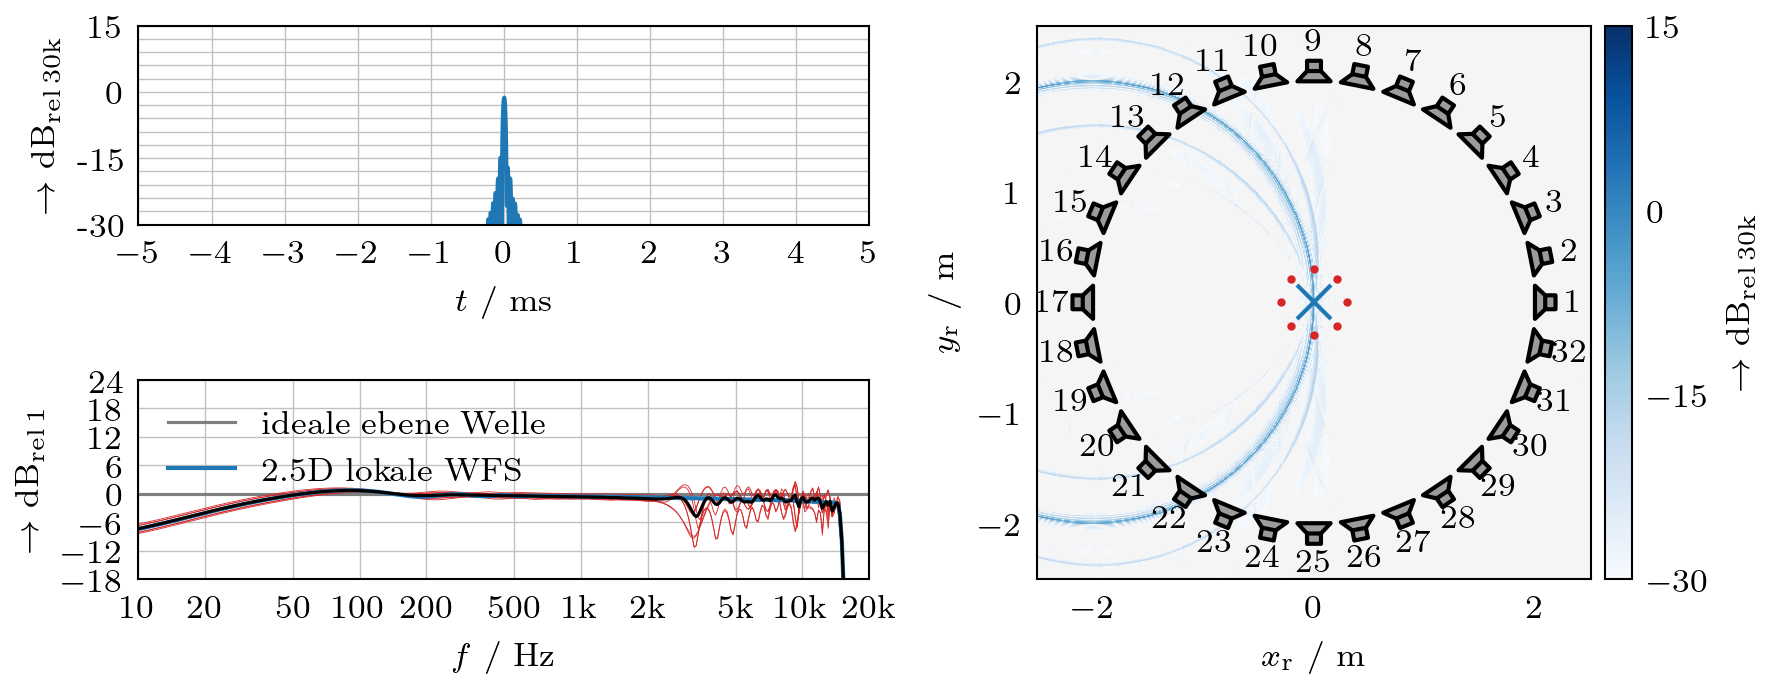
\includegraphics[width=145mm]{../python/lwfs25d_circSSD_time_domain_center_py_DEU.png}
\end{plotfigures}
\caption{2.5D lokale WFS einer lokal planaren, impulshaften
Wellenfront mit Ausbreitung in Richtung positiver $x$-Achse optimiert
für den Referenzpunkt $\times$ bei $\xr=(0,0,0)^\mathrm{T}$\,m.
Wellendurchlauf am Referenzpunkt $\times$ zum gewählten Zeitbezug $t=0$\,s.
Gleiches Setup wie in \Abb\ref{fig:td_0m}; bei lokaler WFS sind alle Lautsprecher
aktiv; Benutzung des idealen 2.5D-WFS-Vorfilters \eqref{eq:Prefilter25D};
%
%Abtastfrequenz $f_s=192$ kHz;
%
Ordnungen für
sphärische Harmonische,
zylindrische Harmonische,
Lagrange-Polynom,
Fourier-Reihe:
$N=30$, $M_s=15$, $\mathcal{M}=5$, $M_a=20$ und
Kaiser-Bessel-Fenster mit $\beta=6$.
%
Im Vergleich zu WFS erzeugt lokale WFS im Referenzpunkt wegen weniger
räumlicher Aliasingartefakte einen linearen Frequenzgang über größeren
Frequenzbereich und eine zeitlich kompaktere Impulsantwort.
%
Frequenzgänge in rot für die rot markierten Messpunkte auf dem Radius $0{,}3$\,m weisen
größere Verzerrungen wegen zeitlich weniger kompakten Impulsantworten auf.
%
Energetisch gemittelter Frequenzgang aus allen Messpunkten in schwarz.
%
\cc
}
\label{fig:td_lwfs_center}
\end{figure*}
%
% please DO NOT rescale the figure and keep it double column
\begin{figure*}[h!]
\centering
\begin{plotfigures}
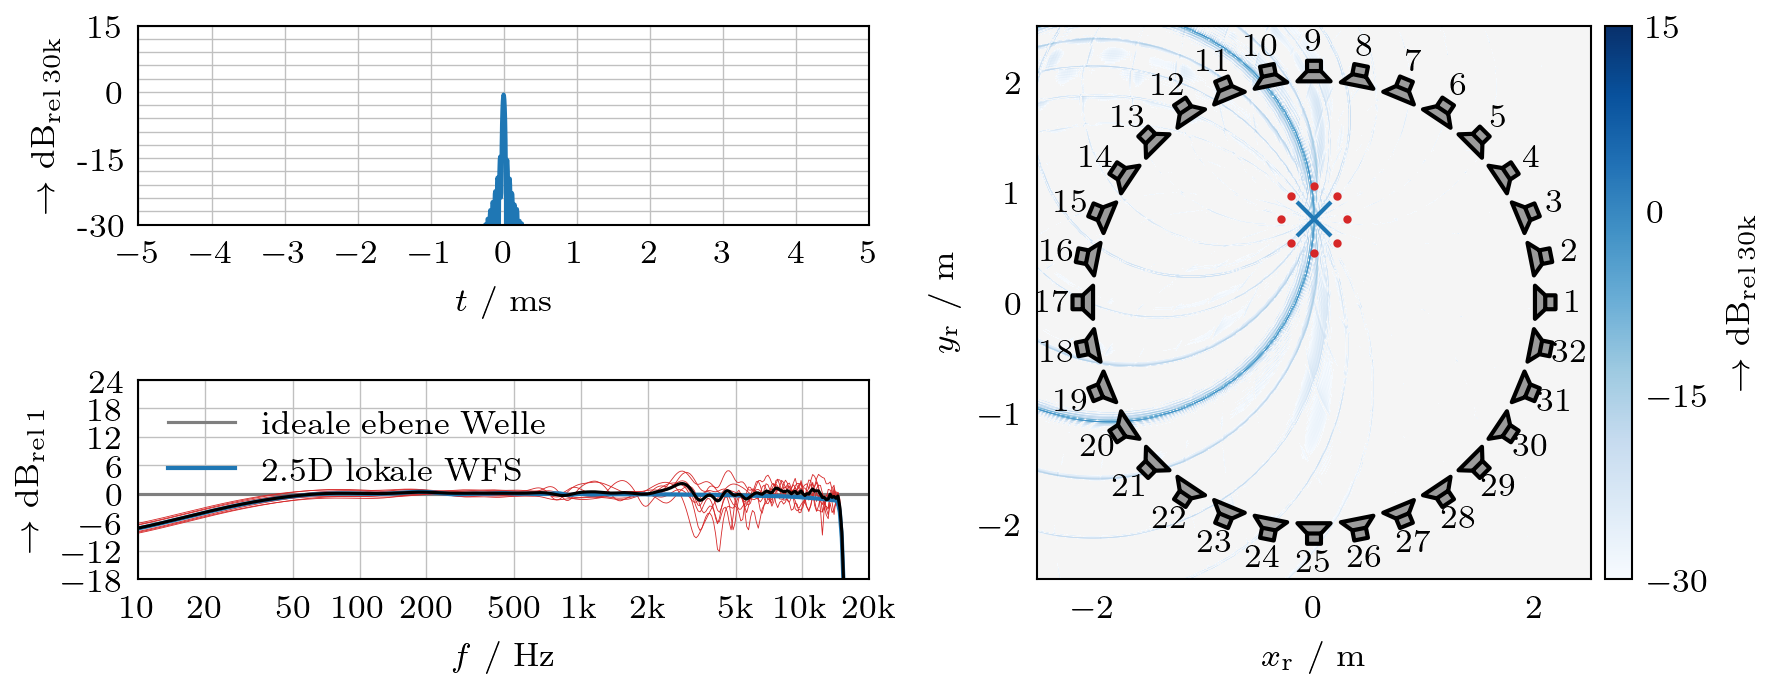
\includegraphics[width=145mm]{../python/lwfs25d_circSSD_time_domain_offcenter_py_DEU.png}
\end{plotfigures}
\caption{2.5D lokale WFS optimiert für den Referenzpunkt
$\times$ bei $\xr=(0,\frac{3}{4},0)^\mathrm{T}$\,m, sonst wie \Abb\ref{fig:td_lwfs_center}.
%
\cc
}
\label{fig:td_lwfs_offcenter}
\end{figure*}
% try to render the 2 figures above on a single page for convenient comparison
% ##############################################################################



\section{Werkzeuge}
\label{sec:WFS_Werkzeuge}
%
WFS-Ansteuerungsalgorithmen für objektorientiertes 3D-Audio mit
echtzeitfähigem Rendering finden sich unter anderem in den folgenden Software-Projekten
\begin{itemize}
\item \cite{url:wonder}, \cite{url:wonder_lite} Derivate der TU Berlin WFS-Software %wonder, Standalone\\\url{https://github.com/dvzrv/wonder}
%\item \cite{url:wonder_lite} %wonder-lite, Standalone\\\url{https://github.com/ntonnaett/wonder}
\item \cite{url:ssr} % Sound Scape Renderer, Standalone\\\url{https://github.com/SoundScapeRenderer}
\item \cite{url:iem-wfs} als VST-Plugin
\item \cite{url:wfscollider} für SuperCollider %WFSCollider für SuperCollider\\\url{https://github.com/GameOfLife/WFSCollider}
\item \cite{url:wfs-diy} für Max %Wave Field Synthesis DIY für Max %\\\url{https://wfs-diy.net/}
\item \cite{Belloch2016_IEEE} für WFS-Rendering auf GPUs
\end{itemize}
%
%Sehr große, dauerhaft installierte WFS-Systeme an Forschungseinrichtungen, die
%mit einem der aufgezählten Renderer arbeiten sind das EMPAC System \cite{Goebel2019}
%(am Curtis R. Priem Experimental Media and Performing Arts Center des Rensselaer
%Polytechnic Institute, in Troy, NY, USA; Rendering mit Max+IRCAM SPAT Revolution)
%und das Wellenfeld H104 System \cite{Baalman2008_diss}
%(Fachgebiet Audiokommunikation, TU Berlin; Rendering mit Eigenentwicklung wonder).
%
Kommerzielle, teils hardware-gebundene Lösungen für WFS sind unter anderem
\begin{itemize}
\item \cite{url:panoramix} Stand-Alone-Software für post production
\item \cite{url:spat_revolution} für Max %IRCAM SPAT Revolution für Max\\\url{https://forum.ircam.fr/projects/detail/spat/}
\item \cite{url:flux_spat_revolution}, optionale WFS-Lizenz; Stand-Alone, oder AAX-, AU-, VST-Plugins, oder mit Option für live production, u.a. für Digitalmischpulte %Flux Spat Revolution Ultimate mit Live Production Option, für Digitalmischpulte\\\url{https://www.flux.audio/project/spat-revolution/}
\item \cite{url:iosono} %\& Spatial Audio Workstation %IOSONO inside \& Spatial Audio Workstation\\\url{https://encircled-audio.com/}
\item \cite{url:amadeus_holophonix} (Verwendung von IRCAM SPAT Algorithmik) %Amadeus HOLOPHONIX (benutzt IRCAM SPAT Technologie)\\\url{http://holophonix.xyz/}
\item \cite{url:holoplot} %Holoplot\\\url{https://holoplot.com/}
\end{itemize}
mit mutmaßlich proprietären WFS-Algorithmikerweiterungen.



Sowohl die Benutzerfreundlichkeit,
konsistente Produktionsarbeitsabläufe als auch planare Lautsprecherpanele,
welche mittels Audio-Netzwerken angesteuert werden \cite{Reussner2013_JAES},
vgl. Holoplot, gewinnen an Bedeutung beim Einsatz von WFS für 3D-Beschallungsszenarien.
%
Stand frühe 2020er Jahre scheinen Ambisonics, kanal- und objektbasierter Surround Sound,
sowie kopfhörerbasierte Binauraltechnik
die der WFS bevorzugten 3D-Wiedergabe-Verfahren zu sein.
%
Es ist zu erwarten, dass vermehrt hybride Systeme mit 3D-Ambisonics und 2.5D-~bzw.~3D-WFS
zum Einsatz kommen, um beide Ansätze sinnvoll zu ergänzen.



\vspace{\baselineskip}Alle Grafiken dieses Kapitels sind in \cite{SchultzHahnSpors2023} unter CC BY 4.0 Lizenz verfügbar.
